\documentclass[paper=a4, fontsize=11pt, openany]{book}
% https://stackoverflow.com/questions/491904/how-do-i-remove-blank-pages-coming-between-two-chapters-in-appendix
\usepackage[top=1.8cm, bottom=2.54cm, left=2.25cm, right=2.25cm]{geometry}
\usepackage[utf8]{inputenc}
\usepackage{graphicx} % use includegraphics to import jpegs --- FIXME... see below
\usepackage[british]{babel} % English language/hyphenation
\usepackage{pdfcomment}
\usepackage{amsmath,amsfonts,amsthm} % Math packages
\usepackage{lipsum} % Used for inserting dummy 'Lorem ipsum' text into the template
\usepackage{sectsty} % Allows customizing section commands
\usepackage{color}
\usepackage{parskip}
\usepackage[usenames,dvipsnames,svgnames,table]{xcolor}
%\usepackage[]{nohyperref}  % This makes hyperref commands do nothing without errors
\usepackage{url}  % This makes \url work
% http://tex.stackexchange.com/questions/667/typeset-url-in-a-non-typewriter-font
\urlstyle{same}
% allow manual caption/figure numbering
% http://tex.stackexchange.com/questions/199207/no-caption-number-for-figures-and-tables
\usepackage{caption}
\usepackage{multicol}

\hypersetup{hidelinks}


\usepackage{fourier} % Use the Adobe N-Utopia font for the document - comment this line to return to the LaTeX default

\usepackage{fancyhdr} % Custom headers and footers
\pagestyle{fancyplain} % Makes all pages in the document conform to the custom headers and footers
\fancyhead{} % No page header - if you want one, create it in the same way as the footers below
\fancyfoot[L]{} % Empty left footer
\fancyfoot[C]{} % Empty center footer
\fancyfoot[R]{\thepage} % Page numbering for right footer
\renewcommand{\headrulewidth}{0pt} % Remove header underlines
\renewcommand{\footrulewidth}{0pt} % Remove footer underlines
\setlength{\headheight}{13.6pt} % Customize the height of the header
\numberwithin{equation}{section} % Number equations within sections (i.e. 1.1, 1.2, 2.1, 2.2 instead of 1, 2, 3, 4)
%\numberwithin{figure}{section} % Number figures within sections (i.e. 1.1, 1.2, 2.1, 2.2 instead of 1, 2, 3, 4)
\numberwithin{table}{section} % Number tables within sections (i.e. 1.1, 1.2, 2.1, 2.2 instead of 1, 2, 3, 4)
\setlength\parindent{0pt} % Removes all indentation from paragraphs - comment this line for an assignment with lots of text

% https://www.sharelatex.com/learn/Typesetting_quotations
\usepackage{epigraph}
% \epigraph{All human things are subject to decay, and when fate summons, Monarchs must obey}{\textit{Mac Flecknoe \\ John Dryden}}

\title{Drucksache 1}

\date{2. Auflage, aktualisiert. Jetzt noch deprimierender. Smiley!}

% Mail/Link author?
\author{Claudia Latour / Martin Sonneborn \\
 \textbf{Assange}
}

% allow multi-line comments using \begin{comment} ... \end{comment}
\usepackage{verbatim}



\begin{document}

%% https://tex.stackexchange.com/questions/351540/having-chapters-shown-as-numbers-and-roman-letters
\renewcommand{\thechapter}{\Roman{chapter}}
\renewcommand{\thesection}{\Roman{section}}
\addtolength{\cftsecnumwidth}{10pt}
\addtolength{\cftchapnumwidth}{10pt}

\pagecolor{assangered}\afterpage{\nopagecolor}
\newpagecolor{assangered}\afterpage{\restorepagecolor}

\color{white} % textcolor
\maketitle % Print the title

\pagecolor{assangered}\afterpage{\nopagecolor}
\chapter*{Preface}
\thispagestyle{empty} % No page number on this page
% Dreamworks und Universal sind an einem konzisen Manuskript zum Leben von Julian Assange gescheitert, genauso wie die New York Times und der Guardian.
% Wir auch.
% Nehmen Sie, was jetzt dabei herausgekommen ist, als Plädoyer für Demokratie \& Bürgerrechte (am Beispiel eines Publizisten und Plattformgründers), für eine freie Gesellschaft, freie Presse und freie Information.
% Oder als Sympathieerklärung an das Projekt von WikiLeaks - und Antipathieerklärung an all jene, die es bekämpfen.
\begin{Large}
Dreamworks and Universal have failed to produce a concise manuscript on the life of Julian Assange, as have the New York Times and the Guardian.

So have we.

Take what has now emerged as a plea for democracy \& civil rights (using the example of a publicist and platform founder), for a free society, free press and free information.

Or as a declaration of sympathy for the WikiLeaks project - and antipathy for all those who fight it.
\end{Large}


%% FIXME: FUSS !
\vspace*{\fill}
% Herausgeber:
% Martin Sonneborn
% Fraktionsloses Mitglied des Europäischen Parlaments
% Rue Wiertz 60
% 1047 Brüssel
% Belgien
% 2. Auflage, aktualisiert. Jetzt noch deprimierender. Smiley!
% Die zum Ausdruck gebrachten Meinungen liegen in der alleinigen Verantwortung der jeweiligen Verfasser
% und geben nicht unbedingt den offiziellen Standpunkt des Europäischen Parlaments wieder.
\begin{flushright}
\begin{verbatim}
Editor:
Martin Sonneborn
Non-attached Member of the European Parliament
Rue Wiertz 60
1047 Brussels
Belgium

2nd edition, updated and revised (A.d.H.s: #wise?). Now even more depressing. Smiley!
The opinions expressed are the sole responsibility of the authors and do not necessarily 
reflect the official position of the European Parliament.

This english version has been typeset using LaTeX and has been fully translated by DeepL.com.
A BIG THANK YOU TO deepl.com for the FREE service (This is NON-COMMERICAL, EDUCATIONAL USE!).
Document sources: https://github.com/schnoddelbotz/free-julian-assange
\end{verbatim}
\end{flushright}

\newpage
\color{black}
\thispagestyle{empty} % No page number on this page
\tableofcontents
\thispagestyle{empty} % No page number on this page

\clearpage
%% START 2-column layout == Zweispaltiges Layout. Am ENDE DES DOKUMENTS erfolgt \end...
\begin{multicols}{2}

%% TODO: This should print above chapter 1, not below table of contents.
\epigraph{„Das Politische kann, wo Menschen leben, nicht verschwinden.“ ~ ``The political can, where humans live, not vanish.''}{\textit{J. Habermas}}


%%%%%%%%%%%%%%%%%%%%%%%%%%%%%%%%%%%%%%%%%%%%%%%%%%%%%%%%%%%%%%%%%%%%%%%%%%%%%%%

\chapter{More Being than Appearance}
\pdfcomment{Mehr Sein als Schein
\textCR
Es gehört zu den Erkenntnissen, die einem in Jurisprudenz und Jurisdiktion ungeschulten Beobachter nicht
neu sein dürften, dass die WIRKLICHKEIT eines juristischen VERFAHRENS manchmal nur noch wenig mit der
WIRKLICHKEIT des ihm zugrundeliegenden (RECHTS)
FALLES zu tun hat. Erst recht nicht mit dem DIESEM
wiederum zugrundeliegenden SACHVERHALT. Und am
wenigsten mit der gesellschaftspolitischen und demokratiepraktischen REALITÄT, die sich in ALL DEM konzentriert.
\textCR
Wenn die WIRKLICHKEIT einer GERICHTLICHEN VERHANDLUNG sich von ihrer übergeordneten BEDEUTUNG, von ihren Auslösern, Gründen, Ursachen, Absichten, Zielen \& Folgen - und damit von dem im Grunde
verhandelnswerten POLITISCHEN KERN - vollends
LOSGELÖST hat, um in der absurden SCHEINREALITÄT eines von juristischen Scheinpflöcken eingehegten
Scheingeländes (in unaufhaltsamem Wahnsinn) vor sich
hinzutreiben, dann befindet man sich im Berufungsverfahren um die Auslieferung des WikiLeaks-Gründers
Julian Assange.
\textCR
Womöglich wurden die seit Jahrhunderten durch nichts
als ihr schieres Vorhandensein beglaubigten Prozeduren und Praxen unserer JUSTIZSYSTEME am Ende nun
doch von diesen (selbst)zerstörerischen Ausläufern der
Spätmoderne ereilt - und zwar jeder ihrer noch so aufdringlich zur Schau gestellten HISTORIZITÄTEN zum
Trotz. Das gilt natürlich umso mehr für Großbritanniens
Magna Carta und ihre echtholzvertäfelten Wände, viktorianischen Samtvorhänge, smaragdgrünen Bankierlampen (Art Déco) und (gut gepuderten) Richterperücken.
\textCR
Vor der plakativen Kulisse derartiger „Rechtstraditionen“
sind im gesellschaftlichen Subsystem der Rechtspflege
längst DENKFIGUREN und ARGUMENTATIONSMUSTER entstanden, die (in sonderbarer Selbstreferentialität und blödsinnigster Binnensymbolik) so stur um ihr
EIGENTÜMLICHES EIGENLEBEN kreisen, dass sie mit
gesellschaftlich relevanten Fragen, Zuständen und Implikationen tatsächlich nicht mehr im Entferntesten verbunden sind.}

It is one of the findings that should not be new to an observer untrained in jurisprudence and jurisdiction.
that the REALITY of a legal PROCEDURE sometimes has little to do with the REALITY of the underlying (LAW).
REALITY of the (LAW) CASE on which it is based.
CASE has to do. Especially not with the THESE
in turn underlying ACTUAL CONDUCT. And least
least with the socio-political and democratic-practical REALITY, which is concentrated in ALL THAT.

If the REALITY of a JUDGMENTAL NEGOTIATION is divorced from its overriding MEANING, from its triggers, reasons, causes, intentions, goals \& consequences - and thus from the basically
basically negotiable POLITICAL CORE - completely
in order to be able to live in the absurd SHINING REALITY of a pseudo-territory enclosed by legal
(in unstoppable madness) in front of oneself, then one is
then one finds oneself in the appeal procedure around the extradition of the WikiLeaks founder
Julian Assange.

Possibly, those who for centuries have been driven by nothing
by nothing but their sheer existence of our JUSTICE SYSTEMS have now in the end been
by these (self)destructive offshoots of late modernity.
modernity - and that in spite of all their HISTORICITIES, no matter how obtrusively displayed.
despite. This is of course all the more true for Great Britain's
Magna Carta and its real-wood paneled walls, Victorian velvet curtains, emerald-green banker's lamps (Art Deco) and (well-powdered) judge's wigs.

Against the striking backdrop of such "legal traditions"
in the social subsystem of the administration of justice
and ARGUMENTATION PATTERNS have long since arisen in the social subsystem of the administration of justice, which (in strange self-referentiality and the most stupid internal symbolism) so stubbornly
their OWN OWN LIFE, that they are not able to deal with
socially relevant questions, conditions and implications are actually no longer remotely connected.

\textbf{Like the whole document - This chapter was translated with \url{www.DeepL.com/Translator} (free version)}

%%%%%%%%%%%%%%%%%%%%%%%%%%%%%%%%%%%%%%%%%%%%%%%%%%%%%%%%%%%%%%%%%%%%%%%%%%%%%%%

\chapter{„Yeah, why not?“}
\pdfcomment{Ja, warum nicht?
\textCR
Am 27. und 28. Oktober 2021 wohnen wir in London
einer Verhandlung bei, in der das EIGENTLICH VERHANDELNSWERTE, das ja NIEMALS nur Julian Assange selbst, sondern immer UNS ALLE betroffen hat, erst gar nicht AUSGESPROCHEN wird. Die (seit 1066) minutiös eingeübten Verfahrensregeln wollen es so. Dass hier
nämlich nicht das große Ganze SELBST, sondern nur seine rechtsterminologisch zulässigen WRITS zur Verhandlung stehen. Mit denen nicht das große Ganze SELBST,
sondern nur die von DIESER besonderen BERUFUNG
betroffenen TEILE (s)einer auf juristischem Wege erzeugten „Wirklichkeit“ erfasst werden.
\textCR
Und so kommt es tatsächlich, dass an vollen zwei Verhandlungstagen am höchsten britischen Gericht, dem
Londoner High Court, die im Fall Assange konzentrierte HAUPTFRAGE gar nicht erst auftaucht. Die natürlich
noch immer darin besteht, ob ein angeblich demokratischer Rechtsstaat ein über 100 Jahre altes US-amerikanisches (Anti-)Spionagegesetz zweckentfremden darf,
um - assistiert von traditionsgesättigten Justizapparaten
befreundeter Rechtsstaaten (der alteuropäischen Welt) in einer tausendjährigen Verfolgungsjagd beispiellosen
Ausmaßes einen australischen Publizisten so gründlich
zu vernichten, dass allein das an ihm statuierte Exempel - seiner entfalteten ABSCHRECKUNGSWIRKUNG
wegen - jeglichen Investigativjournalismus einer Vierten
Kraft, die diesen Namen auch nur annähernd noch verdienen will, fortan nachhaltig unterbinden wird.
\textCR
Das britische Bezirksgericht, an dem der australische
Publizist Julian Assange nach einer kafkaesken Kaskade
staatsanwaltlicher (und staatlicher) Manöver im vergangenen Jahr schlussendlich gestrandet war, hatte diese
Frage im Januar d.J. verstörenderweise mit „JA, WARUM
NICHT?“ beantwortet, was den größten demokratischen
SKANDAL in der Geschichte der Demokratie hätte auslösen müssen.
\textCR
Geführt worden war das erstinstanzliche Verfahren (etwas überraschend) von einer biederen Bezirksrichterin
(District Judge) namens Vanessa Baraitser, seinerzeit das
unbeschriebenste Blatt, das die britische Gerichtsbarkeit
zu bieten hatte. Öffentlich bekannt war weder ihr fachlicher Hintergrund noch ihre Vita oder eine Übersicht
der von ihr verhandelten Fälle - noch nicht mal eine verwackelte Photographie. Die durchschnittliche Besitzerin
einer ländlichen Autowaschanlage habe im Netz mehr
Beweise für ihre tatsächliche Existenz hinterlassen als
Vanessa Baraitser, bemerkte der britische Ex-Diplomat
Craig Murray\footnote[1]{Craig Murray über Baraitser: „Jemand schlug mir vor, sie könnte ein Hologramm sein, aber ich denke nicht. Hologramme haben mehr Einfühlungsvermögen.“}.
\textCR
Eine Handvoll Bagatellverfahren waren ihr wohl zugeteilt worden, immerhin aufregend genug für die traditionell aufregungsbereite (britische) Lokalpresse: Sexuelle
Belästigungen von und mit Polizisten, Provinzpolitiker
mit einem Faible für heimliche Handyschnappschnüsse unter vorüberschreitenden Rockträgerinnen, solche
Sachen. In zehn Jahren Bezirksgerichtspraxis hatte Baraitser ein einziges Auslieferungsverfahren verhandelt:
\textCR
Frankreichs Ersuchen nach Überstellung eines in staatliche Korruption um Ex-Präsident Nicolas Sarkozy verwickelten Geschäftsmannes (Alexandre Djouhri). Die
Sache war klar, Baraitser hatte sie zustimmend beschieden.
\textCR
Und nun also der Fall Assange.}

On 27 and 28 October 2021, in London, we will attend
a trial in which the REALLY NEGOTIABLE, which has NEVER only affected Julian Assange himself, but always ALL OF US, is not even TALKED ABOUT. The (since 1066) meticulously rehearsed rules of procedure want it that way. That here
not the big picture ITSELF, but only its legally permissible WRITS are up for negotiation. With which not the great whole ITSELF,
but only the PARTS of a society which are affected by THIS
(s)he parts of a "reality" produced by legal means.

And so it actually happens that on a full two days of hearings at the highest British court, the
London High Court, the MAIN QUESTION concentrated in the Assange case does not even arise. Which of course
is still whether a supposedly democratic constitutional state can misuse a 100-year-old US (anti-)espionage law,
in order to - assisted by tradition-saturated judiciary apparatuses
of friendly states under the rule of law (in the old European world) in a thousand-year chase of unprecedented
Australian publicist so thoroughly that the only thing that could
that the example made of him alone - because of the CRIMINAL EFFECT it has had
investigative journalism of a Fourth Force, which even
Fourth Force that is even remotely worthy of the name will henceforth be permanently prevented.

The British district court in which Australian publicist
Julian Assange after a Kafkaesque cascade of prosecutorial (and governmental)
cascade of prosecutorial (and governmental) manoeuvres last year, the British District Court had
question in January this year with a disturbing "YES, WHY?
NOT?", in what was the biggest democratic
SCANDAL in the history of democracy.

The first instance proceedings were (somewhat surprisingly) conducted by a bland District Judge named Vanessa Barrister.
(District Judge by the name of Vanessa Baraitser, at the time the most
the most undistinguished figure in the British judiciary at the time.
had to offer. Neither her professional background, nor her curriculum vitae, nor an overview of the cases she had heard were publicly known.
of the cases she tried - not even a blurred photograph. The average owner of a rural
of a rural carwash had left more evidence of her actual
more evidence of her actual existence than Vanessa Baraitser
Vanessa Baraitser, noted British ex-diplomat
Craig Murray\footnote[1]{Craig Murray on Baraitser: "Someone suggested to me she might be a hologram, but I don't think so. Holograms have more empathy."}.

A handful of small claims cases had probably been assigned to her, exciting enough for the traditionally excitable (British) local press, after all: Sexual
sexual harassment by and with police officers, provincial politicians
with a penchant for surreptitious mobile phone snaps among pre-crossing skirt wearers, that sort of thing.
Stuff. In ten years of district court practice, Baraitser had heard a single extradition case:

France's request for the rendition of a businessman (Alexandre Djouhri) implicated in state corruption surrounding ex-president Nicolas Sarkozy. The
The matter was clear, Baraitser had approved it.

And now the Assange case.


%%%%%%%%%%%%%%%%%%%%%%%%%%%%%%%%%%%%%%%%%%%%%%%%%%%%%%%%%%%%%%%%%%%%%%%%%%%%%%%

%\pdfcomment{}
\chapter{Real criminal shit} % III.
\pdfcomment{Echt krimineller Shit
\textCR
Bevor irgendjemand sich irgendein Urteil über Julian
Assange bildet, sollte er sich noch einmal in Erinnerung
rufen, mit wem (und mit was) er es da eigentlich zu tun
hat.
\textCR
Fleißige Statistiker haben ausgerechnet, dass die kleine Gruppe von Aktivisten um WikiLeaks in zehn Jahren
ZEHN MILLIONEN Geheimdokumente veröffentlicht
hat. Mehr als die gesamte Weltpresse, seit es die gesamte
Weltpresse überhaupt gibt. Dokumente über Kriegsverbrechen, Menschenrechtsverletzungen, Folter, Gewalt,
Entführungen, illegale Überwachung, Spionage, Meinungsmanipulation und Umweltverbrechen.
\textCR
Einschlägige Veröffentlichungen umfassen diplomatische und militärische Geheimpapiere (führender kriegführender Staaten) sowie Dokumente zur Sichtbarmachung der Vorgehensweisen gesellschaftswirksamer
Organisationen und Einzelakteure - (verlogene) Regierungen, (machtbesessene) Parteiapparate, (korrupte)
Politiker, (unsympathische) Unternehmer, (Arschloch-)
Konzerne und (notorische) Egomanen, (Schweizer)
Banken, (Offshore-)Betrüger, (profitfixierte) Naturzerstörer und schließlich politische („Hillary“) und religiöse
(„Scientology“) Sekten. WikiLeaks-Publikationen waren
dabei nie Selbstzweck, sondern Mittel zur Erreichung
eines zutiefst demokratischen Ziels, das - getragen von
einem ganz schön altmodischen Menschheits- und Gesellschaftsideal\footnote[2]{Aufklärung!} - auf die (unumstößliche) Überzeugung
zurückgeht, dass eine FREIE GESELLSCHAFT nur auf
FREIER INFORMATION gegründet sein kann.
\textCR
Im Projekt von WikiLeaks verdichtet sich die grundlegende Frage moderner Demokratien, nämlich die nach
der LEGITIMIERBARKEIT von staatlichen, nachrichtendienstlichen und militärischen Informationsmonopolen.
\textCR
WikiLeaks stellt Fragen, die jeder mündige 
Bürger\footnote[3]{Im Sinne Kants, Voltaires, Daisy Ducks \& R.D. Prechts} sich
und seinen demokratischen Repräsentanten (und -onkeln) stellen sollte: Hat eine Regierung das Recht, sich
(mit dem Ziel des Machterhalts oder der Bereicherung)
über geltendes Recht hinwegzusetzen? Hat ein Nachrichtendienst das Recht, die Persönlichkeitsrechte von
Bürgern zu verletzen, zu deren Schutz er bestellt ist?
Hat ein Militär das Recht, gegen Menschenrechte oder Prinzipien des Völkerrechts zu verstoßen? Und, falls ja,
haben diese Organisationen zudem noch das Recht, ihre
Rechtsverstöße durch Geheimhaltung vor der Öffentlichkeit zu verbergen?
\textCR
Assange, ein mehrfach preisgekrönter Journalist und
Verleger, wird seit April 2019 rechtsgrundlos im britischen Hochsicherheitsgefängnis Belmarsh festgehalten
- zusammen mit Terroristen und Schwerverbrechern,
Serienmördern, Sexualstraftätern, Islamisten, Rechtsextremisten, IRA-Kämpfern und Christoph Waltz, der
als Ernst Stavro Blofeld von hier aus zuletzt sein bionisches Auge einsetzte, um den (fehlschlagenden) Befehl
zur Tötung von James Bond zu geben. Belmarsh ist das
britische Guantanamo, eine streng geometrische Zuchtanstalt mit klinisch weißen Innenzellen, ein Ort, der den
(treffenden) Spitznamen HELLMARSH trägt. Hier sitzt
der WikiLeaks-Gründer seit 30 Monaten in Einzelhaft trotz wiederholter Erklärungen der Vereinten Nationen
(und anderer), wonach er Opfer willkürlicher, illegaler Inhaftierung und psychologischer Folter ist. Es gibt,
das muss man sich immer wieder klar machen, KEINE
RECHTSGRUNDLAGE für die Inhaftierung von Julian
Assange. In Großbritannien liegt nicht das Geringste
gegen ihn vor.
\textCR
\textit{Sachdienlicher Hinweis von Ross Kemp
Nachdem wir Teile der Dokumentation „Welcome to
HMP Belmarsh“ gesehen haben, für die der Schauspieler
Ross Kemp („EastEnders“) erstmals Drehgenehmigung
und Zugang zum Hochsicherheitsgefängnis erhalten hatte, sind wir fast ein bisschen erleichtert, dass Assange dort
wenigstens in einem Einzelzimmer untergebracht ist.
Und wir sind entsetzt, wirklich fassungslos, dass man ihn
seiner Freiheit beraubt, um ihn ohne Rechtsgrundlage an
einen solchen Ort zu zwingen. Ross Kemp ist ein Mann wie
ein Wohnzimmerschrank und ziemlich hart im Nehmen.
Weltweit hat er schon unter kriminellen Straßengangs, in
Afghanistan, Papua-Neuguinea und werweißwonoch als
„embedded journalist“ gedreht, ohne mit einer einzigen
Wimper zu zucken. Als er „The Box“, die Hochsicherheitseinheit des Gefängnisses, betritt und sich nur kurz die
Tür hinter ihm schließt, ist er am bedrückendsten Ort der
ganzen Welt, sagt er. Es gibt kein Bett, kein Waschbecken,
keine Toilette, kein Fenster, keinen Zugang zu Wasser oder
zu Luft. „Man spürt, dass man völlig allein ist. Ich glaube
nicht, dass ich eine Stunde hier drin verbringen könnte,
ohne wahnsinnig zu werden.“}
\textCR
Im erstinstanzlichen Verfahren um seine Auslieferung
hatte Bezirksrichterin Baraitser sich verbissen geweigert,
jeden der auf der Hand liegenden Sachverhalte auch nur
zur Kenntnis zu nehmen - vom genuin JOURNALISTISCHEN Charakter der Veröffentlichungen von WikiLeaks
über die erkennbar POLITISCHE Natur der gegen seinen
Gründer gerichteten Anwürfe bis hin zur (wirklich auch für Blinde) offensichtlichen Aussicht auf ein unfaires Gerichtsverfahren in den USA.
\textCR
Assange würde in ALEXANDRIA im US-Bundesstaat Virginia vor Gericht gestellt werden, wo er sich einem geheimen Verfahren vor einem Sondergericht mit Grand
Jury stellen müsste. In unmittelbarster Nähe dieser
Stadt, in Washington und Langley, befinden sich das
Pentagon, die Defense Intelligence Agency, das FBI, die
CIA, die NSA sowie die Hauptquartiere weiterer Militär-,
Sicherheits- und Geheimdiensteinrichtungen der USA.
Die Einwohnerstruktur von Alexandria ist von einer
durchschnittlichen Stadtbevölkerung in etwa so weit
entfernt wie dieser lächerliche Prozess hier von einem
rechtsstaatlichen Verfahren. Zwischen 80 und 90 Prozent
der volljährigen Bewohner Alexandrias, unter denen die
Laienrichter im Verfahren gegen Assange rekrutiert würden, sind Vertreter von Regierungsbehörden, Geheimdiensten oder des US-Militärs und stehen in einem direkten, indirekten oder (wenigstens) wirtschaftlichen
Abhängigkeitsverhältnis zur US-Regierung. Grand Jurys
im zuständigen Gerichtsbezirk sind so zuverlässig einäugig, einohrig, einseitig, parteiisch und voreingenommen, dass man eine objektive Urteilsfindung von ihnen nicht ernsthaft erwarten kann - die Loyalitätslast
gegenüber der Regierung ist erdrückend. In der langen
Geschichte des Eastern District Court of Virginia gab es
noch nie auch nur einen einzigen Fall, in dem die Grand
Jury einen von den nationalen Sicherheitsbehörden Angeklagten freigesprochen hätte. Wirklich noch nie.
\textCR
\textit{Sachdienlicher Hinweis von heise.de
US-amerikanische Rechtsvereinigungen wie die American Association of Jurists (AAJ) und das Center for Constitutional Rights (CCR) haben gemeinsam mit international arbeitenden juristischen Institutionen und Juristen
einen Brief an den britischen Premierminister Boris Johnson und seine Regierung geschrieben, um ihn von einer
Auslieferung Julian Assanges an die USA abzuhalten. Ein
solcher Schritt wäre ihrer Ansicht nach illegal:
„Die Auslieferung wäre rechtswidrig, da der Schutz der
grundlegenden Prozessrechte von Herrn Assange in den
USA nicht gewährleistet ist. Herr Assange wird vor dem
berüchtigten „Spionagegericht“ des Eastern District of
Virginia (in Alexandria, die Verf.) vor Gericht gestellt, vor
dem kein Angeklagter der nationalen Sicherheit jemals
Erfolg hatte. Hier sieht er sich einem geheimen Verfahren vor einer Jury ausgesetzt, die aus einer Bevölkerung
ausgewählt wurde, in der die meisten Personen, die für
die Auswahl der Jury in Frage kommen, für die CIA, NSA,
DOD oder DOS (The Central Intelligence Agency, The National Security Agency, U.S. Department of Defense, U.S.
Department of State) arbeiten oder mit dieser verbunden
sind.“}}

Before anyone makes any judgement about Julian
Assange, he should remind himself once again who (and what) he is
who (and what) they are actually dealing with.
they are dealing with.

Diligent statisticians have calculated that in ten years the small group of activists around WikiLeaks have published
TEN MILLION secret documents in ten years.
in ten years. More than the entire world press, since the entire
world press has even existed. Documents about war crimes, human rights violations, torture, violence,
kidnappings, illegal surveillance, espionage, manipulation of opinion and environmental crimes.

Relevant publications include diplomatic and military secret papers (of leading belligerent states) as well as documents to make visible the modus operandi of socio-economic organisations and individual actors.
organisations and individual actors - (lying) governments, (power-obsessed) party apparatuses, (corrupt) politicians
(corrupt) politicians, (unsympathetic) entrepreneurs, (arsehole)
corporations and (notorious) egomaniacs, (Swiss)
(Swiss) banks, (offshore) fraudsters, (profit-fixated) nature destroyers and finally political ("Hillary") and religious
("Scientology") sects. WikiLeaks publications were
never an end in itself, but a means to achieve a deeply
of a profoundly democratic goal, which - borne out of
and social ideal\footnote[2]{Enlightenment!} - is based on the (incontrovertible) conviction that a FREE
that a FREE SOCIETY can only be based on
FREE INFORMATION.

In the WikiLeaks project, the fundamental question of modern democracies is condensed, namely that of
the LEGITIMACY of state, intelligence and military information monopolies.

WikiLeaks is asking questions that every responsible 
citizen[3]{in the sense of Kant, Voltaire, Daisy Duck \& R.D. Precht} should ask himself and his democratic
and his democratic representatives (and uncles): Does a government have the right to
(with the aim of retaining power or enriching itself)
override the law? Does an intelligence service have the right to violate the privacy rights of citizens?
of citizens it has been appointed to protect?
Does a military have the right to violate human rights or principles of international law? And, if so,
do these organisations also have the right to conceal
violations from the public through secrecy?

Assange, a multi-award-winning journalist and publisher, has been
publisher, has been held without legal grounds in the UK's maximum security Belmarsh prison since April 2019
- along with terrorists and serious criminals,
serial killers, sex offenders, Islamists, right-wing extremists, IRA fighters, and Christoph Waltz, who was
as Ernst Stavro Blofeld, last used his bionic eye from here to execute the (failed) order to kill James Bond.
to kill James Bond. Belmarsh is the
British Guantanamo, a strictly geometric breeding facility with clinically white interior cells, a place that has been given the
(aptly) nicknamed HELLMARSH. Here sits
the WikiLeaks founder has been held in solitary confinement for 30 months despite repeated statements by the United Nations
(and others) that he is a victim of arbitrary, illegal detention and psychological torture. There are,
must be made clear time and time again that there is NO
LEGAL BASIS for the detention of Julian
Assange. There is nothing whatsoever
against him.

\textit{Subjective note from Ross Kemp.
After watching parts of the documentary "Welcome to
HMP Belmarsh", for which actor
for which actor Ross Kemp ("EastEnders") was granted filming
and access to the high security prison, we are almost a little relieved that Assange is at least housed in a single room.
at least in a single room.
And we are appalled, really stunned, that he should be deprived of his
of his liberty to force him into a place like this
to a place like this without any legal basis. Ross Kemp is a man like
like a living room cupboard, and he's pretty tough.
All over the world he has worked among criminal street gangs, in
Afghanistan, Papua New Guinea and who knows what else as an
"as an embedded journalist without batting an eyelid.
without batting an eyelid. When he enters "The Box", the prison's high-security unit, and the door closes behind him, he is on the edge of his seat.
closes behind him, he is in the most oppressive place in the whole world, he says.
whole world, he says. There is no bed, no sink,
toilet, no window, no access to water or air.
to air. "You feel you are completely alone. I don't think
I don't think I could spend an hour in here
without going insane."}

In the first-instance proceedings concerning his extradition
District Judge Baraitser had stubbornly refused to allow any of the
refused to even take note of any of the obvious facts.
of the obvious facts - from the genuinely JOURNALISTIC nature of WikiLeaks' publications
to the recognisably POLITICAL nature of the accusations against its
founder, to the obvious (to the blind, really) prospect of an unfair trial in the USA.

Assange would be tried in ALEXANDRIA in the US state of Virginia, where he would have to face a secret trial in a special court with a grand
grand jury. In the immediate vicinity of this
Washington and Langley, are the Pentagon, the Defense
the Pentagon, the Defense Intelligence Agency, the FBI, the
CIA, the NSA, and the headquarters of other military,
security and intelligence agencies of the United States.
The population structure of Alexandria is
is about as far from an average urban population
as this ridiculous trial is from the rule of
from the rule of law. Between 80 and 90 per cent
of Alexandria's residents of legal age, among whom the lay
lay judges in the Assange trial would be recruited are representatives of government agencies, intelligence services or the US military, and have a direct, indirect or (at least) economic relationship of dependence on the US government.
relationship of dependence on the US government. Grand juries
in the relevant judicial district are so reliably one-eyed, one-eared, one-sided, biased and prejudiced that they cannot seriously be expected to render an objective verdict - the burden of loyalty
to the government is crushing. In the long
the Eastern District Court of Virginia, there has
there has never been a single case in which the grand jury has
grand jury acquitted a defendant brought by the national security agencies. Truly never.

\textit{Subjective note from heise.de
US legal associations such as the American Association of Jurists (AAJ) and the Center for Constitutional Rights (CCR), together with legal institutions and jurists working internationally, have written a letter to the British Prime Minister.
have written a letter to British Prime Minister Boris Johnson and his government to dissuade him from extraditing Julian Assange to the US.
Julian Assange from being extradited to the USA. A
Such a move would, in their view, be illegal:
"Extradition would be unlawful because the protection of Mr.
of Mr Assange's fundamental due process rights in the
is not guaranteed in the USA. Mr Assange will be tried before the
notorious "spy court" of the Eastern District of
Virginia (in Alexandria, the author), before which no accused
before which no national security defendant has ever succeeded.
ever succeeded. Here, he faces a secret trial before a jury selected from a population in which most of the
population in which most of the persons eligible for jury
eligible for jury selection work for the CIA, NSA,
DOD or DOS (The Central Intelligence Agency, The National Security Agency, U.S. Department of Defense, U.S.
Department of State) work for or are affiliated with.
}


%%%%%%%%%%%%%%%%%%%%%%%%%%%%%%%%%%%%%%%%%%%%%%%%%%%%%%%%%%%%%%%%%%%%%%%%%%%%%%%

\chapter{„Reeeevenge!“ (Fatty Pompeo)} % 4
\pdfcomment{„Raaache!“ (Fatty Pompeo)
\textCR
Den Vereinigten Staaten von Amerika war Assange nach
der Veröffentlichung der (vom US-Militär penibel unter
Verschluss gehaltenen) Materialien zu den Kriegen im
IRAK und in AFGHANISTAN spätestens mit den Publikationen zu Menschenrechtsverletzungen im Gefangenenlager Guantanamo Bay verbindlich auf die Zehen
getreten\footnote[4]{(Aua, aua.)}.
\textCR
Unter Barack OBAMA hatten die USA noch auf eine
Anklage gegen Assange verzichtet - nicht aus Menschenfreundlichkeit, sondern eines handfesten Definitionsdilemmas wegen, das unter Juristen als das
„New-York-Times-Problem“ bekannt ist. Es geht ungefähr so: Wie kann man Julian Assange wegen der Veröffentlichung von als geheim eingestuftem Material (auf
den Seiten von WikiLeaks) verfolgen - NICHT ABER die
Chefredakteure der New York Times, auf deren Seiten
doch GENAU DASSELBE stand? Oder die Herausgeber
von The Guardian, Le Monde, El Pais, Corriere della Sera,
Süddeutsche Zeitung oder Der Spiegel?
\textCR
Damit hier nicht (aus Versehen) ein falscher Eindruck
entsteht: Unter der Regierung Obama sind die US-amerikanischen Geheimdienste und Justizbehörden natürlich ebenfalls gegen Assange vorgegangen. 2011 hat das
FBI eine großangelegte Infiltrationsoperation gegen WikiLeaks in Island durchgeführt, einen Pädophilen als falschen Zeugen angeworben und - in Vorbereitung einer
Anklage - bereits die passende Grand Jury einberufen.
Vorläufig zurückgestellt wurde lediglich die Einleitung
eines Verfahrens, und dies nur auf dringendes Anraten
von Rechtsanwälten, denen (im Weißen Haus) schlagartig der Inhalt des „First Amendment“ eingefallen war.
\textCR
Den feinsinnigen Rechtsphilosophen um Donald
TRUMP ging diese Sache mit der fehlenden Trennschärfe (zwischen Publizisten und Publizisten) freilich am
Arsch vorbei.
\textCR
2017 hatte WikiLeaks die (beunruhigenden) Fähigkeiten
des amerikanischen Geheimdienstes zu elektronischer
Überwachung und Cyber-Kriegsführung öffentlich gemacht. Das sogenannte „Vault 7“-Leak war das „größte“ und - der New York Times zufolge - wirklich auch
das „peinlichste“ Datenleck, das der CIA je passiert war
- oder einem ihrer Behördenleiter. Für den damaligen
CIA-Chef (und späteren Außenminister) Mike Pompeo
mag es (darüber hinaus) eine (narzisstische) Kränkung
gewesen sein (oder nicht). Jedenfalls war es der Auslöser
für eine seither mit allen nur denkbaren Mitteln geführte
(Privat-)Vendetta gegen WikiLeaks und Julian Assange.
Fatty Pompeo wollte RACHE. Und erklärte WikiLeaks offiziell zum „feindlichen nichtstaatlichen Geheimdienst“
- eine seinem Erfinder an plumper Bösartigkeit in nichts nachstehende Begriffsneuschöpfung, von der kein seriöser Staatsrechtler zuvor (oder seitdem) jemals gehört
hat.\footnote[5]{Die Pressekonferenz, in der Pompeo WikiLeaks diesen feierlichen Ehrentitel erklärt, wird von rückblickenden
Politikwissenschaftlern als einer der kardinalen Wendepunkte markiert werden müssen, an dem die (post-)
demokratische Ordnung der westlichen Welt ihrem dialektischen Umschlagspunkt ins Auge sah.}
\textCR
Mit Trump und Pompeo im Rücken erhob das US-Justizdepartment schließlich seine waghalsige Anklage gegen
Julian Assange. Die Schrift umfasst 18 Punkte (das sind
mehr als ein westeuropäischer Marienkäfer hat) und
stellt ihm nach Auslieferung eine Haftstrafe von 175 Jahren in Aussicht - je zehn Jahre für jeden der 17 Anklagepunkte unter dem Espionage Act und weitere fünf für
den 18., in dem ihm das versuchte Eindringen in einen
Regierungscomputer unterstellt wird, ein Verstoß nach
dem „Computer Fraud and Abuse Act“.
\textCR
Noch einmal zur Erinnerung: KEIN EINZIGER der USamerikanischen Kriegsverbrecher, die im Irak, Afghanistan oder Guantanamo erwiesenermaßen ihr Unwesen
getrieben, Unschuldige, Zivilisten, Kinder gequält, gefoltert und ermordet hatten, wurde für sein Verbrechen
je zur Rechenschaft gezogen, angeklagt oder vor Gericht
gestellt. Sie alle sind auf freiem Fuß. Zur Rechenschaft
gezogen, angeklagt und vor Gericht gestellt werden soll
hier der, der ihre Verbrechen öffentlich gemacht hat.
\textCR
Die Vereinigten Staaten stützen sich dabei im wesentlichen auf den Espionage Act, ein Gesetz aus dem Jahr
1917, das unter Weltkriegsbedingungen für Weltkriegsgeheimnisträger und Weltkriegsinformationen von weltkriegsmilitärischer Sensibilität entwickelt wurde - wo
hat die Division General Custer ihre Haubitzen geparkt?
Allein diese in Ermangelung eines plausiblen, justiziablen (oder sonstwie stichhaltigen) Tatvorwurfs hervorgekramte „Rechtsgrundlage“ müsste jedem der PRÄMODERNE geistig entwachsenen Europäer (gründlich) zu
denken geben. Der Versuch, ein überholtes Kriegsgesetz
über 100 Jahre später völlig kontextenthoben gegen einen ausländischen Publizisten zur Anwendung zu 
bringen\footnote[6]{Selbstverständlich wurde es schon zu Zeiten des Ersten Weltkriegs von der US-Justiz zweckentfremdet, um Vertreter der politischen Opposition, Sozialisten oder Pazifisten zum Schweigen zu bringen. 
Eine Praxis, die die USA bis in die späten Sechziger Jahre (und darüber hinaus) beibehalten sollten. Aufsehen erregte etwa der 1971 (gescheiterte) Prozess gegen die Militäranalysten Daniel Ellsberg und Anthony Russo, die der New York Times, Washington Post u.a. Dokumente überlassen hatten, die belegen, dass die US-Regierung die Öffentlichkeit seit
Jahren über den Vietnamkrieg belogen hatte („Pentagon Papers“).}, entspricht der putzigen Idee des Irren vom Bosporus, eine zeitgenössische Satire von Jan Böhmermann
mit dem reichsdeutschen Majestätsbeleidigungsgesetz
(anno 1871) zur Strecke zu bringen. Beides ist schon
auf den allerersten Blick so abwegig, dass es keines umständlicheren Kommentars dazu bedarf. Wir halten fest:
Es gibt keine Rechtsgrundlage, um einen australischen
Journalisten nach dem US-Spionagegesetz vor Gericht
zu stellen.
\textCR
Die US-Anklage ist nicht nur völlig aus der Zeit gefallen
und absolut absurd, sie ist auch wirklich verfassungswidrig, denn sie kriminalisiert die 
journalistische Kernaktivität und hebt damit jahrhundertealte Rechtsgrundsätze auf, allen voran das der Rede- und natürlich das
der Pressefreiheit.}

The United States of America was not aware of Assange's
the publication of the materials (meticulously kept under wraps by the
materials on the wars in the IRAQ and AFGHANISTAN.
IRAQ and AFGHANISTAN, at the latest with the publications on human rights violations in the Guantanamo Bay prison camp.
stepped\footnote[4]{(Ouch, ouch.)}.

Under Barack OBAMA, the USA had still refrained from
not out of philanthropy, but because of a tangible definitional dilemma, known among lawyers as the "New York Times problem".
"New York Times problem". It goes something like this: how can Julian Assange be prosecuted for publishing classified material (on the pages of
the pages of WikiLeaks) - BUT NOT the editors of the
editors-in-chief of the New York Times, on whose pages
said EXACTLY THE SAME THING? Or the editors
of The Guardian, Le Monde, El Pais, Corriere della Sera,
Süddeutsche Zeitung or Der Spiegel?

Lest a false impression be created here (by mistake)
Under the Obama administration, the US intelligence and judicial authorities have, of course, also taken action against Assange. In 2011 the
FBI carried out a large-scale infiltration operation against WikiLeaks in Iceland, recruited a paedophile as a false witness and - in preparation for an indictment - had already selected the appropriate grand jury.
and - in preparation for an indictment - has already convened the appropriate grand jury.
The only thing that has been postponed for the time being is the
proceedings have been postponed, and this only on the urgent advice
of lawyers who (in the White House) had suddenly remembered the contents of the "First Amendment".

The subtle legal philosophers around Donald
TRUMP didn't give a damn about the lack of distinction (between publicists and publicists).
ass.

In 2017, WikiLeaks had revealed the (disturbing) capabilities of the American
of the American secret service to electronic
surveillance and cyber warfare. The so-called "Vault 7" leak was the "biggest" and - according to the New York Times - really also the "most
the "most embarrassing" data leak that had ever happened to the CIA
- or any of its agency heads. For the then
CIA chief (and later Secretary of State) Mike Pompeo
it may (or may not) have been a (narcissistic) slight.
(or not). In any case, it was the trigger
for a (private) vendetta against the US that has since been carried out
(private) vendetta against WikiLeaks and Julian Assange.
Fatty Pompeo wanted ACHIEVEMENT. And officially declared WikiLeaks a "hostile non-state intelligence agency".
- a neologism every bit as crude and malicious as its inventor, and one that no serious constitutional lawyer has ever heard of before (or since).
\footnote[5]{The press conference in which Pompeo declares WikiLeaks to have this ceremonial title of honour is considered by retrospective political scientists to be one of the most cardinal events in the history of the United States.
political scientists as one of the cardinal turning points at which the (post-) democratic
democratic order of the Western world faced its dialectical tipping point}.

With Trump and Pompeo behind it, the US Justice Department finally brought its audacious indictment of
Julian Assange. The writ covers 18 points (that's
more than a western European ladybird has) and
and, if he is extradited, it offers him the prospect of 175 years in prison - ten years for each of the 17 counts under the Espionage Act and a further five for the 18th count on which he was convicted.
for the 18th, which charges him with attempting to hack into a government
computer, an offence under the Computer Fraud and Abuse
Computer Fraud and Abuse Act.

Again, as a reminder, NONE of the US war criminals proven to have been at large in Iraq, Afghanistan or Guantanamo have been innocent, civilians, or children.
tortured, tortured and murdered innocent people, civilians, children, was ever held accountable for his crime.
ever been held accountable, charged or tried for his crime.
tried. They are all at large. Accountable
The one who should be held accountable, charged and brought to justice is the one
here is the one who made their crimes public.

The United States essentially relies on the Espionage Act, a law passed in
1917, developed under World War II conditions for World War II secretaries and World War II information of World War II military sensitivity - where
did General Custer's division park its howitzers?
This "legal basis" alone, dug up in the absence of a plausible, justiciable (or otherwise valid) accusation of an offence, should give every European who has mentally outgrown the PRE-MODERNE (thorough) food for thought.
think. The attempt to make an obsolete law of war
more than 100 years later against a foreign publicist completely out of context 
6]{Of course, it was already misused by the US judiciary during the First World War to silence representatives of the political opposition, socialists or pacifists. 
A practice that the USA was to maintain until the late 1960s (and beyond). The 1971 (failed) trial of military analysts Daniel Ellsberg and Anthony Russo, who had given documents to the New York Times, Washington Post and others proving that the US government had been lying to the public for years about the Vietnam War, caused a stir.
years about the Vietnam War ("Pentagon Papers")}, corresponds to the cute idea of the madman from the Bosporus, a contemporary satire by Jan Böhmermann
with the Reichsdeutsche Majestätsbeleidigungsgesetz (Imperial German libel law)
(anno 1871). Both are already
so absurd at first glance that there is no need for a more long-winded commentary. We hold:
There is no legal basis to prosecute an Australian journalist under the
Australian journalist under the US Espionage Act.
under the US Espionage Act.

The US prosecution is not only completely out of time
and absolutely absurd, it is also genuinely unconstitutional, because it criminalises core journalistic 
journalistic core activity and thus abrogates centuries-old legal principles, first and foremost that of freedom of speech and, of course, that of the
freedom of the press.


%%%%%%%%%%%%%%%%%%%%%%%%%%%%%%%%%%%%%%%%%%%%%%%%%%%%%%%%%%%%%%%%%%%%%%%%%%%%%%%

\chapter{Ping, Pong \& Psychology} % V. = 5
\pdfcomment{Ping, Pong \& Psychologie
\textCR
Dennoch hatte Bezirksrichterin Baraitser nach mehrwöchiger Verhandlung die irrwitzige Auffassung vertreten, der Auslieferung Assanges stünde nicht die OFFENSICHTLICHE UNGEHEUERLICHKEIT einer mit
protojuristischen Winkelzügen konstruierten Anklageschrift entgegen, sondern lediglich - Tätärääää! - die
nach sieben Jahren Isolation in der Ecuadorianischen
Botschaft und weiteren zweieinhalb Jahren rechtsgrundloser Inhaftierung (ziemlich überraschungsfrei)
in Mitleidenschaft geratene psychische Verfassung des
zu Unrecht festgehaltenen Häftlings. Ergänzt um dessen
manifeste Suizidgefährdung, die durch die in aller Welt
bekannten US-amerikanischen Haftbedingungen samt
ihrer gewohnheitsmäßigen Bestialität vorhersehbar verstärkt würde.
\textCR
Bei Assange, so Baraitsers Urteil, liege ein prekärer psychischer Zustand vor, der sich angesichts der „harten
Bedingungen“ des unmenschlichen US-Gefängnissystems verschlechtern würde, was ihn „zum Selbstmord
veranlassen“ könne. Rule, Britannia.
\textCR
Dabei lässt Baraitsers Urteil die haarsträubenden
„Rechtsgründe“ der USA, die ein ECHTES FANGIRL des
britannischen Rule of Law kunstfertig in der Luft hätte
zerreißen müssen, fatalerweise völlig unangetastet - und
bestätigt, indem sie sie nicht ausdrücklich verwirft, damit implizit ihre Zulässigkeit. Das ist echt krass. Noch
krasser ist eigentlich nur, dass ihr Urteil das Verhandlungsgeschehen vom SCHLACHTFELD der PRESSEFREIHEIT, die natürlich alle Demokraten und Bürger
und Menschen der Welt betrifft, auf die Ebene einer individuellen SCHICKSALSBEURTEILUNG transponiert,
in der just nicht mehr das große Ganze einer gefährdeten Gesellschaftsordnung, sondern nur mehr die technischen und interpretativen Details medizino-psychologischer Gutachten eine Rolle spielen.
\textCR
Allein das war und ist (ohne jeden Zweifel) ein rechtsstaatlicher Skandal. Und zwar ein multipler. Hugh.
\textCR
Ein WEITERER kommt nun dadurch hinzu, dass das
hier (nachgelagert) geführte BERUFUNGSVERFAHREN im engmaschigen Netz des von der ersten Instanz vorgegebenen Begründungsrahmens gefangen ist - und die
gerichtliche Erörterung sich nahezu vollumfänglich auf
das unerschöpflich vage (\& zudem zuverlässig persönlichkeitsverletzende) Feld der PSYCHOLOGIE begibt.
\textCR
Und so kommt es tatsächlich, dass die anwaltlichen
Ausführungen im bedeutendsten Rechtsstreit zur Pressefreiheit der Gegenwart sich auf ein PING PONG aus
substanzfreien Unterstellungen, küchenpsychologischen Mutmaßungen und deren fachgemäßer Widerlegung reduzieren. VORGEBRACHT von James Lewis (in
der Rolle des PING), einem versierten Schießhund der
Krone, der hier natürlich nicht im Dienste Seiner Majestät, sondern höchst unfeiner Beschwerdeführer aus den
USA steht. Und WIDERLEGT von Edward Fitzgerald \&
Mark Summers (Team PONG), zwei mit derlei Blödsinn
sichtlich unterforderte Menschenrechtsanwälte auf Seiten der Verteidigung.
\textCR
Sollte die Encyclopaedia Britannica je einen Eintrag zum
Begriff „groteske Dysfunktionalitäten archaotraditionalistischer Rechtssysteme“ planen, hätten wir da einen
Knoten im Taschentuch, den wir bestimmt nie vergessen
werden. Knoten ist im Taschentuch, Ihr Vögel. Knot is in
the handkerchief. You birds.}

Nevertheless, after several weeks of trial, District Judge Baraitser had taken the ludicrous view that Assange's extradition was not prevented by the OPENLY INCREDIBLE nature of an indictment constructed with proto-legal dodges.
of a bill of indictment constructed with proto-legal dodges, but only - Tätärääää! - the
after seven years of isolation in the Ecuadorian Embassy
embassy and another two and a half years of unlawful imprisonment (rather unsurprisingly).
the mental condition of the unjustly detained prisoner.
unjustly detained prisoner. Supplemented by his
suicidal tendencies, which were exacerbated by the world-renowned
conditions of imprisonment in the USA
and its habitual bestiality.

According to Baraitser's judgement, Assange is in a precarious mental state which, in view of the "harsh conditions" of the inhumane
conditions" of the inhumane US prison system, which could "cause him to commit suicide".
to commit suicide". Rule, Britannia.

In doing so, Baraitser's judgement leaves out the hair-raising
"legal grounds" of the USA, which a REAL FANGIRL of the
of the British Rule of Law, which should have been artfully
fatally left completely untouched - and
by not explicitly rejecting it, implicitly confirms its admissibility. That's really crass. Even more
even more crass is the fact that her judgement shifts the negotiating process from the BATTLEFIELD of PRESS FREEDOM, which of course concerns all democrats and citizens
and people of the world, to the level of an individual SHOCKSHIP,
in which precisely the big picture of an endangered social order no longer plays a role, but only the technical and interpretative details of medico-psychological reports.

This alone was and is (without any doubt) a scandal of the rule of law. And a multiple one at that. Hugh.

A FURTHER one is now added by the fact that the
(downstream) proceedings here are caught in the tightly woven net of the framework of reasons given by the first instance - and the
and the judicial discussion is almost entirely based on the inexhaustibly vague
the inexhaustibly vague (\& furthermore reliably personality-infringing) field of PSYCHOLOGY.

And so it is indeed the case that the lawyer's
in the most important legal dispute on the freedom of the press of the present day, is a PING PONG of insinuations without
of insinuations without substance, kitchen-sink psychological conjectures and their expert refutation. PRESENTED by James Lewis (in the
the role of PING), an accomplished gun dog of the
Crown, who here, of course, is not in the service of His Majesty but of highly unsubtle complainants from the
USA. And WIDERLEGED by Edward Fitzgerald \&.
Mark Summers (Team PONG), two human rights lawyers clearly under
clearly underchallenged with such nonsense.

Should the Encyclopaedia Britannica ever have an entry on the
term "grotesque dysfunctionalities of archaotraditional legal systems", we would have a knot in the
a knot in our handkerchief that we will certainly never forget.
ever forget. Knot is in the handkerchief, you birds. Knot is in
the handkerchief. You birds.


%%%%%%%%%%%%%%%%%%%%%%%%%%%%%%%%%%%%%%%%%%%%%%%%%%%%%%%%%%%%%%%%%%%%%%%%%%%%%%%

\chapter{In the wood-panelled heart of power} % 6
\pdfcomment{Im holzvertäfelten Herzen der Macht
\textCR
Das Gerichtsgebäude der Royal Courts of Justice in der
Londoner Innenstadt ist ein ehrgebietender Ort voll
säkularer Sakralität und vollholzgepflasterter Gerichtssaalminiaturen. Hier kommen - nach der letzten Reform
von 1873 (HÖRT, HÖRT!) - nicht nur die bedeutendsten
Common-Law-Gerichte einschließlich des Höchsten
und des Berufungsgerichts zusammen, sondern in einer
winzigen Trachtenstube namens COURT ROOM FOUR\footnote[7]{Der Court Room Four soll so etwas wie der persönliche Gerichtssaal des Lord Chief Justice sein. Hier findet er
alles, was ihm nur lieb sein kann: eine Brise Atemluft aus der Kolonialzeit, seine gemütlichsten Puschen und 1
paar Motten, die beides überlebt haben.} also auch besagter Anklagevertretervertreter James Lewis (Perücke: Langhaar, Ziege) sowie Edward Fitzgerald
(Langhaar, Ross) und Mark Summers (Langhaar, unecht),
die Verteidiger von Julian Assange (Langhaar, echt).
\textCR
Ihre rabenschwarzen Roben reichen bis zu den Spitzen
ihres jeweiligen Schuhwerks herunter, was sich - zumindest nach ein paar Pints - als potentiell halsbrecherische Tradition entpuppen könnte. Spätestens seit der
Studentenbewegung dürfte allgemein bekannt sein, was
UNTER DEN TALAREN in aller Regel so verborgen ist,
hier ist das alles 300 Jahre alt. Seine schmutziggrauen
Flechtperücken verdankt der feine Londoner Anwaltsstand übrigens noch nicht einmal selbstbestimmtem
Schöpfergeist oder Boris Johnson, sondern (im Gegenteil) einer kontinentaleuropäischen Raubkopie König
Karls II., der den Einfall zur Herstellung handgeknüpfter Zweitfrisuren 1660 ausgerechnet aus Frankreich importierte. (Get Brexit done, folks, schon klar. Oder in den
Worten Monty Pythons: “Isch ’abe keine Lust, länger mit
dir zu reden, du verkarkter englischer Frischbiertrinker!
Ich furze auf euch, ihr Schweinepriester! Wenn es nach
mir geht, kommt ihr nicht in Europäische Gemeinschaft!“)
\textCR
Den Anwälten gegenüber präsidieren Lord Justice Sir
Timothy Victor Holroyde (Robe, Kurzhaar, schwarze
Gesichtsmaske) und Lord Chief Justice of England and
Wales Lord Ian Duncan Burnett, Baron Burnett of Maldon (Robe, Kurzhaar, maskenlos). Ob das Coronavirus
in Großbritannien im Oktober 2021 noch existiert oder
nicht, wird vom Höchsten Gericht dem Anschein nach
etwas widersprüchlich beurteilt. Die Pubs auf der Insel
(und all ihre Besucher) sind sich in dieser Frage längst
einig, was aus Sicht eines Kontinentaleuropäers eine
surreale, aber keineswegs unangenehme Reminiszenz
an eine Zeit auslöst, in der man unter Coronae noch die
kreisförmigen Oberflächenstrukturen entfernter Planeten verstand.
\textCR
So oder so nehmen die obersten Hüter des Rechtssystems Ihrer Majestät auf exzentrisch roten Polstersesseln Platz, alle anderen in der plebejisch-proletarischen
Holzklasse, die mit den mittelalterlichsten Bänken ausgestattet ist, die seit der Enthauptung Ann Boleyns JEMALS von Menschen besessen wurden. Allein sie natürlich eine so spartanische wie subtile körperliche Folter,
die den fiesesten Kolonialplünderern aller Zeiten durchaus angemessen ist\footnote[8]{Nach den Belgiern, eigentlich. Aber Schwamm drüber.}.
\textCR
Auf den Holzklassebänken der Gerichtssaal-Empore
lassen sich auch Assanges Vater John Shipton, seine Verlobte Stella Moris, der derzeitige WikiLeaks-Chefredakteur Kristinn Hrafnsson sowie WikiLeaks-Botschafter
Joseph Farrell nieder - neben der Handvoll Journalisten
und Prozessbeobachter, die es in den VIP-Bereich dieser
Besuchertribüne geschafft haben. Übrigens über eine
waghalsig gewundene Wendeltreppe im Inneren eines
schmalen Foltertürmchens UND an einer wortkargen
Gerichtsbilleteuse vorbei.}


The Royal Courts of Justice courthouse in the centre of
London is an awe-inspiring place full of secular
secular sacredness and all-wood courtroom miniatures. Here - after the last reform
of 1873 (LISTEN, LISTEN!) - not only the most important common law
common law courts, including the Supreme
and the Court of Appeal, but also in a
tiny dressing room called COURT ROOM FOUR\footnote[7]{Court Room Four is supposed to be something like the Lord Chief Justice's personal courtroom. Here he finds
everything that can be dear to him: a breath of colonial air, his cosiest slippers, and 1
a few moths that have survived both} so also said prosecuting counsel James Lewis (wig: longhair, goat) as well as Edward Fitzgerald
(longhair, steed) and Mark Summers (longhair, fake),
the defence lawyers for Julian Assange (longhair, real).

Their raven black gowns reach down to the tips
of their respective footwear, which - at least after a few pints - could turn out to be a potentially breakneck tradition. At the latest since the
student movement at the latest, it should be common knowledge what
under the talars is usually so hidden,
here it's all 300 years old. His dirty grey
the fine London legal profession owes its dirty grey wigs not even to a self-determined
or Boris Johnson, but (on the contrary) to a pirated continental European copy of King Charles II.
Charles II, who imported the idea of producing hand-knotted secondary hairstyles in 1660 from France, of all places. (Get Brexit done, folks, all right. Or in the
Or in the words of Monty Python: "I don't want to talk to you any more
to talk to you any longer, you overgrown English fresh beer drinker!
I'll fart on you, you swine priests! If it's up to
If it's up to me, you won't get into the European Community!")

Presiding over the lawyers are Lord Justice Sir
Timothy Victor Holroyde (robe, short hair, black face mask)
face mask) and Lord Chief Justice of England and Wales
Wales Lord Ian Duncan Burnett, Baron Burnett of Maldon (robe, short hair, maskless). Whether the coronavirus
still exists in Great Britain in October 2021 or not
or not in the UK in October 2021 is, on the face of it.
somewhat contradictory. The pubs on the island
pubs (and all their patrons) have long been in agreement on this
which, from the point of view of a continental European, is a
surreal, but by no means unpleasant, reminiscence of a time
of a time when coronae still meant the circular surface structures
the circular surface structures of distant planets.

Either way, the supreme guardians of Her Majesty's legal system take their seats on eccentric red upholstered armchairs, everyone else in the plebeian-proletarian
wooden class, furnished with the most medieval benches EVER possessed by man since the beheading of Ann Boleyn. She alone, of course, a physical torture as spartan as it is subtle,
quite befitting the nastiest colonial plunderers of all time\footnote[8]{After the Belgians, actually. But bygones be bygones}.

On the wooden class benches of the courtroom gallery
Assange's father John Shipton, his fiancée Stella Moris, the current WikiLeaks editor-in-chief Kristinn Hrafnsson, and WikiLeaks ambassador
Joseph Farrell - along with the handful of journalists and trial
and trial observers who made it into the VIP section of this
visitors' gallery. Incidentally, via a
spiral staircase inside a narrow torture tower.
inside a narrow torture tower AND past a taciturn courtroom
court billeteuse.

%%%%%%%%%%%%%%%%%%%%%%%%%%%%%%%%%%%%%%%%%%%%%%%%%%%%%%%%%%%%%%%%%%%%%%%%%%%%%%%

\chapter{Who is there - and who is not} % 7
\pdfcomment{
Wer da ist - und wer nicht
\textCR
Der Zugang zur Public Gallery war initial, warum auch
immer, einem strengen Reglement und drastischer Kontingentierung ausgesetzt gewesen, bevor im Laufe zweier Verhandlungstage allmählich KAIROS übernahm, der
Gott des günstigen Augenblicks. Wer zur richtigen Zeit
am richtigen Ort das richtige Gesicht aufsetzte\footnote[9]{Und die richtige Parole dabeihatte.}, wurde eingelassen. „Lassen Sie mich durch, ich bin die EU.“
Wer nicht, der eben nicht. Platz gewesen wäre hier für
100 Personen, wenn die wortkarge Billeteuse nicht nach
einem guten Dutzend, warum auch immer, die schwere
Gerichtstür knirschend hinter sich zugezogen hätte.
\textCR
Ein Dutzend Plätze also für die interessierte Öffentlichkeit. Für eine Verhandlung, in der die interessierte Öffentlichkeit selbst zur Disposition steht.
\textCR
Alle anderen Prozessbeobachter, in der Hauptsache Vertreter etwas unbedeutend klingender Medien, müssen
die Verhandlung per Videoübertragung aus einem entlegenen Gerichtssaal verfolgen - über Bildschirme, auf
denen man nichts sieht, und Lautsprecher, aus denen
man nichts hört. Weitere 80 Journalisten weltweit zeigen
diesmal immerhin Zeichen von Interesse, indem sie sich
über einen Videolink zuschalten lassen.
\textCR
Die meisten von ihnen sind gar nicht erst angereist, weil
das britische Gerichtswesen im Vorfeld nicht dazu in der
Lage gewesen war, ihnen den Zutritt zum Verhandlungssaal zuzusichern. Pressevertreter erhielten widersprüchliche Nachrichten, monatelang war der zuständige, ein
namenloser Gerichtsangestellter im Urlaub gewesen
(lange) oder erkrankt (schwer), verzogen, versetzt, verletzt oder verstorben (unerwartet), und hatte auf Anfragen daher gar nicht erst geantwortet - schon gar nicht
verbindlich. Einlassgarantien wurden kategorisch verweigert, Presseakkreditierungen nicht vergeben, Zugangslisten nicht geführt.
\textCR
Wer also ein Pressevertreter und trotzdem - aufs Geratewohl - in dieses Londoner Gerichtsgebäude gekommen
ist, der ist ein FREAK. Wäre er es nicht, würde er unter
derartigen Bedingungen kaum erschienen sein. Die unbestechliche und durch nichts zu entmutigende Regisseurin, Publizistin und Aktivistin Angela Richter ist hier,
(immerhin) im Auftrag des Feuilletons der WELT, der
gescheite Daniel Ryser vom Schweizer Magazin REPUBLIK, Markus Kompa verfolgt das Geschehen für TELEPOLIS (übers Laptop auf einer Mülltonne vor dem Gerichtsgebäude) - und das war’s auch schon fast.
\textCR
Gesandte bedeutenderer, auflagestärkerer deutschsprachiger \& internationaler Medienhäuser - oder gar
die großen Nachrichtenagenturen selbst - sind natürlich nicht zugegen. Wir nehmen an: AUS GRÜNDEN.
Und unterstellen ihnen getrost, dass sie AUCH NICHT
gekommen wären, wenn man ihnen Luxus-Suiten mit
privatem Ginbrunnen, diamantbesetzte Giveaways oder
den Kronschatz irgendeiner Majestät (an)geboten hätte.
\textCR
Bedeutende Medienhäuser interessieren sich nämlich
nicht für Assange, müssen Sie wissen. Jedenfalls nicht
mehr. Als sie seine Veröffentlichungen noch für irgendwelche idiotischen Titelseitenknaller ausschlachten
konnten, interessierten sie sich natürlich AUCH NICHT
für ihn. Oder für WikiLeaks. Oder wenigstens für das
Prinzip der PRESSEFREIHEIT, das zwar ihre eigene Existenzberechtigung begründet, an seinen wirklich ENTSCHEIDENDEN KIPPUNKTEN von ihnen aber trotzdem
immer NUR andeutungsweise verteidigt wird.
\textCR
Wenn es stattdessen nun von jemandem verteidigt werden muss, und zwar BUCHSTÄBLICH mit seinem EIGENEN LEBEN, ohne dass einschlägige Medienheinis sich
dafür besonders interessierten, dann wissen wir eigentlich auch nicht weiter. Sollten die Prinzipien der Demokratie BRENNBAR sein, betrachten wir sie hiermit als
ENTZÜNDET.
\textCR
NICHT zugegen sind natürlich auch jene - nach Selbstauskunft - demokratieaffinen Bürgerrechts-Militanten
aus den verwinkelten Strukturen der Europäischen Union. Kein einziger offizieller Vertreter des EU-Parlaments,
kein einziger der zweiunddreißigtausend Beamten der
EU-Kommission, kein einziges Mitglied irgendeines
gar nicht hoch genug zu überschätzenden Ausschusses
für „bürgerliche Freiheiten oder was“, keine korrupte
kroatische Kommissarin für „Demokratie und Demographie“, kein Beauftragter für die Trümmer des (europäischen) Menschenrechts. Kein einziger dieser EU-bürokratischen Schmierlapps, die es für gewöhnlich gar
nicht erwarten können, sich in irgendeine dramatische
PR-Pose zu werfen, sobald irgendwo von PRESSEFREIHEIT oder MENSCHENRECHTEN die Rede 
ist\footnote[10]{Zwei irische Kollegen aus dem Europaparlament sind da: Clare Daly und Mick Wallace. Nicht im Auftrag des
Parlaments, sondern (wie wir) in eigener Sache. Einige halten sie für links, andere für radikal, die meisten wohl
für beides. Es ist ganz egal, denn das Wichtigste, was man als Bürger wissen muss, ist, dass sie wirklich nichts
im Auge haben als das Wohl (der Mehrheit) der Menschen (nicht nur) in der EU. Gäbe es nur Abgeordnete wie
diese beiden hier, dann müssten die (mindestens) 25.000 (feinen) Brüsseler Lobbyisten ihre (mindestens)
11.000 (feinen) Lobbyisten-Läden dichtmachen. Und zwar für immer.}.
\textCR
Wie sich auch an diesem Beispiel wieder zeigt, geht es
EU-Vertretern offensichtlich weniger um die verteidigenswerten Prinzipien von Pressefreiheit und Menschenrechten selbst als um deren politische Instrumentalisierbarkeit.
\textCR
Immerhin hatte das EU-Parlament sich gerade erst kollektiv aufgeplustert, um einem nicht grundlos umstrittenen, weil letztlich eben rechtsradikaloiden Spinner wie
Alexei KRAWALNY seinen dümmlichen Sacharow-Preis
zu verleihen. Nun ja. Angesichts der Reihe seiner bisherigen Träger ordnen wir diesen schlecht dotierten PLASTEPOKAL nicht dem LOBPREIS von IRGENDWAS (Menschenrecht, Demokratie, Pressefreiheit) zu, sondern der
(derzeit viel angesagteren) Kategorie „hybride Kriegsführung“. Und während das EU-Parlament einmal im
Jahr damit zuverlässig seine SCHÄRFSTE (wenn auch völlig irrelevant gebliebene) medien- und moralpolitische (Android-) Waffe in Stellung bringt, bringt es seit
einem Jahrzehnt noch immer kein Sterbenswörtchen
zum Fall Assange zustande. Keine (vordergründige) moralische Empörung, keine (hohle) politische Forderung,
noch nicht einmal ein (bedeutungs- oder folgenfreier)
kleiner Kommentar.
NICHT AUSZUDENKEN, was in den Hirnen dieser europäischen Werteträger und Demokratiekämpfer wohl los
wäre, hätten nicht die Vereinigten Staaten von Amerika,
sondern der Iran, Russland oder - Gott behüte - CHINA
die Auslieferung eines Journalisten verlangt, der nichts
getan hat, als wahrheitsgemäße Information über (von
diesen) begangene (Kriegs-)verbrechen zu veröffentlichen. Großes rhetorisches Feuerwerk, olympische Blitzbündel und Donnerkeile usw., der Dritte Weltkrieg stünde uns bevor. Gute Güte!}


For whatever reason, access to the Public Gallery had initially been
and drastic quota system, before KAIROS, the god of the opportune moment, gradually took over in the course of two days of negotiations.
the god of the opportune moment. Whoever put on the right face
the right face at the right place at the right time[9]{and had the right slogan with him} was let in. "Let me through, I am the EU."
Those who don't, don't. There would have been room for
100 people, if the taciturn billeteuse hadn't asked for a good
a dozen or so, for whatever reason, the heavy court door
the heavy courtroom door creaking shut behind her.

A dozen seats for the interested public. For a trial in which the interested public itself is up for disposition.

All other observers of the trial, mainly representatives of somewhat insignificant-sounding media, must
the trial by video transmission from a remote courtroom - via screens on which nothing can be seen, and loudspeakers.
screens from which nothing can be seen and loudspeakers from which
from which nothing can be heard. A further 80 journalists from around the world
show signs of interest this time by tuning in via a video link.
by tuning in via a video link.

Most of them have not even travelled to the event because
the British judiciary had not been able to grant them access.
had not been able to guarantee them access to the courtroom. Members of the press received conflicting messages, and for months the court clerk in charge, an
unnamed court clerk had been on holiday for months
(for a long time) or ill (seriously), moved, injured or deceased (unexpectedly), and had therefore not even responded to enquiries - certainly not in a binding manner.
bindingly. Admission guarantees were categorically refused, press accreditations not issued, access lists not kept.

Anyone who is a representative of the press and nevertheless - at random - comes to this London courthouse is a FREAK.
is a FREAK. If he were not, he would hardly have
would hardly have appeared under such conditions. The incorruptible and undaunted director, publicist and activist Angela Richter is here,
(after all) on behalf of the feuilleton of the WELT, the
The clever Daniel Ryser from the Swiss magazine REPUBLIK, Markus Kompa follows the events for TELEPOLIS (via laptop on a dustbin in front of the courthouse) - and that's almost it.

Envoys of more important, higher-circulation German-language \& international media houses - or even
the big news agencies themselves - are of course not present. We assume: FOR REASONS.
And confidently assume that they would ALSO NOT have come
if they had been offered luxury suites with a private
private gin fountain, diamond-studded giveaways or the crown treasure
the crown treasure of some majesty.

Major media houses are not interested in Assange, you know.
in Assange, you must know. At least not
anymore. When they could still exploit his publications for some idiotic front-page bombshells
they were of course NOT interested in him either.
in him. Or for WikiLeaks. Or at least for the
principle of FREEDOM OF THE PRESS, which, although it justifies their own existence, is nevertheless always ONLY vaguely defended by them at its really DECISIVE POINTS.
is always defended ONLY insinuatingly.

If, instead, it has to be defended by someone, and that BOOSTINGLY with his OWN LIFE, without the relevant media people being particularly interested in it
interested in it, then we don't really know what to do. If the principles of democracy should be FIREABLE, we hereby consider them to be
DESTROYED.

NOT present, of course, are those - according to their self-declaration - democracy-savvy civil rights militants
from the convoluted structures of the European Union. Not a single official representative of the EU Parliament,
not one of the thirty-two thousand officials of the
EU Commission, not one single member of any
committee on "civil liberties", which cannot be overestimated
for "civil liberties or what", not a single corrupt
Croatian commissioner for "democracy and demography", no commissioner for the rubble of (European) human rights. Not a single one of these EU bureaucratic greasepainters who usually can't wait to get
can't wait to throw themselves into some dramatic
dramatic PR pose as soon as PRESS FREEDOM or HUMAN RIGHTS are mentioned anywhere. 
is\footnote[10]{Two Irish colleagues from the European Parliament are here: Clare Daly and Mick Wallace. Not on behalf of the
Parliament, but (like us) on their own behalf. Some consider them left-wing, some radical, most probably both.
both. It doesn't matter, because the most important thing to know as a citizen is that they really have nothing
than the welfare of (the majority of) the people (not only) in the EU. If there were only MEPs like
these two here, then the (at least) 25,000 (fine) lobbyists in Brussels would have to pay their (at least)
11,000 (fine) lobbyist shops shut down. And for good}.

As this example again shows, EU representatives are obviously less
EU representatives are obviously less concerned with the defensible principles of press freedom and human rights themselves than with their political instrumentalisation.

After all, the EU Parliament had only just puffed itself up collectively in order to give a not without reason controversial, because ultimately radical right-wing nutcase like
Alexei KRAWALNY his stupid Sakharov Prize.
prize. Well, yes. In view of the series of its previous recipients, we do not assign this poorly endowed PLASTEPOKAL to the LOBPREIS of IRGENDWAS (human rights, democracy, freedom of the press), but to the
(currently much more fashionable) category "hybrid warfare". And while the EU Parliament once a
year, the EU Parliament reliably brings into position its most severe (albeit completely irrelevant) media- and morality-political (android) weapon.
a decade, it has still not been able to utter a word
about the Assange case. No (superficial) moral outrage, no (hollow) political demand,
not even a (meaningless or consequence-free)
little comment.
NOT TO THINK what would be going on in the brains of these European value bearers and democracy fighters if the United States of
would be, if not the United States of America,
but Iran, Russia or - God forbid - CHINA
demanded the extradition of a journalist who had done nothing
but truthful information about (war-) crimes committed by these
(war) crimes committed by them. Big rhetorical fireworks, Olympic lightning bolts and thunderbolts etc., World War III would be upon us. Good grief!

%%%%%%%%%%%%%%%%%%%%%%%%%%%%%%%%%%%%%%%%%%%%%%%%%%%%%%%%%%%%%%%%%%%%%%%%%%%%%%%

\chapter{Castorf and the living knee}
\pdfcomment{Castorf und das lebende Knie
\textCR
Assange wurde die PERSÖNLICHE TEILNAHME an dem
Berufungsverfahren, das über den Rest seines Lebens
entscheiden wird, übrigens ohne Angabe von Gründen
verwehrt. Ein WEITERER UMSTAND, der diese Gerichtssitzung zu einer Farce macht. Deutlicher könnte ein
Rechtswesen kaum zeigen, was es von den (humanistischen) Traditionsbeständen hält, die es an höheren Feiertagen immer so qualvoll beschwört.
\textCR
Über Assange wird hier verhandelt, disputiert und gemutmaßt wie über eine WARE, ein Klumpen ENTRECHTETER MATERIE, dem es noch nicht einmal gestattet
ist, dem dadaistischen Detailhandel über seine eigenen
EXPORTBEDINGUNGEN beizuwohnen. Der Angeklagte
als absentes Objekt spezialisierten Experteninteresses,
über den (oder das) Anwesende in albernen Perücken
nach Belieben verfügen können. Habeas corpus 2.0.
\textCR
Es wirkt wie eine frühe Inszenierungsidee von Frank
Castorf, wenn unscharfe Bewegtbilder des ABWESENDEN zu Beginn des ersten Verhandlungstages plötzlich
auf längsseitig platzierten Monitoren erscheinen. Sie
zeigen Assange im BLUE ROOM des HMP Belmarsh, Her
Majesty’s Prison: acht Quadratmeter einer Gummizelle,
achtzehn Kilometer LUFTLINIE vom Ort des hiesigen
Rechtsgeschehens entfernt.
\textCR
SAGEN kann der, um dessen (blankes) Leben es geht,
hier freilich nichts. Auch lachen, schreien, die Stirn in
tektonische Verzweiflungsfalten legen, sich mit seinen
Anwälten besprechen, in den Gang der Verhandlung
eingreifen kann der, den sie betrifft, mitnichten. WENN
Assange erscheint, dann erscheint er als SPRACHLOSER
BEISITZER seines eigenen Lebenslaufs, fachanwaltlicher Brillanz \& höchstrichterlichen Gnadenakten ausgeliefert; 
eingefangen (ausgerechnet) von einer Überwachungskamera mit deaktiviertem Mikrophon.
\textCR
Man wünschte kurz, es gäbe GÖTTER, das alles zu zerschlagen.
\textCR
Diese nur wenige Minuten dauernde Bewegtbild-Zuschaltung eines zu TOTALER PASSIVITÄT VERDAMMTEN VERHANDLUNGSOBJEKTS ist die vielleicht klarste
Metapher für das, was aus diesem Verfahren geworden
ist.
\textCR
Es ist zugleich das Dokument der psychischen und physischen Zerstörung eines Menschen. Am Tag vor Verhandlungsbeginn hatten Gefängnisärzte Ihrer Majestät
Art, Dosierung oder Zuschnitt der Assange verabreichten
Medizin verändert, WAS AUCH IMMER man in einem
Hochsicherheitsgefängnis unter Medizin versteht (und
WARUM AUCH IMMER man so etwas auf den Vorabend
einer Gerichtsverhandlung legt). „Hohe Dosis Medikamente“, murmelt ein Richter. Wie Assange aussah, ist
bereits beschrieben worden, wir wollen es gar nicht erst
versuchen. Hager, blass, müde, jedenfalls nicht gut.
\textCR
Wenn er beim Betreten der Videozelle sichtlich taumelt auf dem Weg zu einem Tisch, vor dem eine Kamera ohne
Mikrophon installiert ist, und wenn er - am Tisch sitzend
- immer wieder schwach zu zittern und für Sekundenbruchteile zu zucken beginnt, müde, bevor er das halb
verdeckte Gesicht auf eine Hand stützt wie auf eine rettende Insel, kann man sich nur noch EINES fragen: Was
zum Teufel soll das alles?
\textCR
Nach wenigen Minuten zieht Assange sich in einen hinteren Winkel der Zelle zurück; (es ist) die einzige selbstbestimmte Entscheidung, die ihm noch geblieben ist. Er
entzieht sich dem starren Kamerakegel, zurück bleibt
ein leerer Tisch, ein leerer Stuhl und - ab und an vom
rechten äußersten Bildrand zugeschaltet: ein (lebendes)
Knie.
\textCR
Konsequenterweise verzichtet das lebende Knie am
zweiten Verhandlungstag auf sein Recht auf Live-Zuschaltung zum dargebotenen Castorf-Stück.}


Assange has been denied PERSONAL PARTICIPATION in the
appeal proceedings, which will decide the rest of his
the rest of his life, without giving any reasons.
denied. A FURTHER CONSTITUTION that makes this court session a farce. A legal system could hardly show more clearly
legal system could hardly show more clearly what it thinks of the (humanistic) traditions it always so agonisingly invokes on high holidays.

Assange is being negotiated, disputed and conjectured about as if he were a commodity, a lump of LEGITIMATE MATERIAL that is not even allowed to be sold to the Dadaist retail trade.
not even allowed to tell the dadaist retail trade about its own
EXPORT CONDITIONS. The accused
as an absent object of specialised expert interest,
over whom (or which) those present in silly wigs can
can dispose of at will. Habeas corpus 2.0.

It seems like an early staging idea of Frank
Castorf, when blurred moving images of the ABSTAINER at the beginning of the first day of the trial suddenly appear
appear on monitors placed lengthwise. They
show Assange in the BLUE ROOM of HMP Belmarsh, Her
Majesty's Prison: eight square metres of a padded cell,
eighteen kilometres AWAY from the scene of the local legal
legal events here.

The person whose (bare) life is at stake can SAY,
can say nothing here. Nor can they laugh, scream, frown in tectonic
in tectonic folds of despair, discuss the matter with his
with his lawyers, intervene in the course of the trial.
can intervene in the course of the trial. IF
Assange appears, then he appears as a LACK OF SPEECH
HIS own curriculum vitae, at the mercy of specialist lawyers' brilliance \& supreme court acts of mercy; 
captured (of all things) by a surveillance camera with a deactivated microphone.

One briefly wishes there were GODS to smash it all.

This moving image feed, lasting only a few minutes, of a NEGOTIATING OBJECTIVE DAMNED TO TOTAL PASSIVITY is perhaps the clearest
metaphor for what this process has become.
has become.

It is also the document of the psychological and physical destruction of a human being. On the day before the trial began, Her Majesty's Prison Doctors had
changed the type, dosage or cut of medicine given to Assange.
medicine, WHATEVER is understood to be medicine in a high-security prison.
in a maximum-security prison (and why
WHY, WHY, WHY, WHY, WHY, WHY, WHY, WHY, WHY, WHY, WHY
of a trial). "High dose of medication," murmurs one judge. What Assange looked like has
already been described, we won't even try.
try. Gaunt, pale, tired, certainly not well.

When he visibly staggers upon entering the video cell on his way to a table in front of which a camera is installed without a
microphone is installed, and when he - seated at the table
- table, he begins to tremble faintly and twitch for fractions of a second, tired, before resting his half-covered face on a hand.
half-covered face on one hand as if on a saving island, one can only ask ONE thing: What the hell is all this?
the hell is this all about?

After a few minutes, Assange retreats to a back corner of the cell; (it is) the only self-determined decision left to him. He
the stare of the camera, leaving behind an empty table
an empty table, an empty chair and - now and then from the far right
from the far right edge of the picture: a (living) knee.
knee.

Consistently, the living knee renounces its right to be
on the second day of the trial, the living knee waives its right to a live link to the Castorf play being performed.

%%%%%%%%%%%%%%%%%%%%%%%%%%%%%%%%%%%%%%%%%%%%%%%%%%%%%%%%%%%%%%%%%%%%%%%%%%%%%%%

\chapter{Lawyer of the week}
\pdfcomment{Anwalt der Woche
\textCR
Wenn sie dran sind, stehen Ankläger und Verteidiger,
beide Q.C.\footnote[11]{Was in diesem Fall leider nicht die Abkürzung für Qualitätskontrolle (Quality Control), überhöhte Ladegeschwindigkeit (Quick Charge) oder wenigstens einen Webcomic (Questionnable Content) ist, sondern für einen Anwalt der Krone (Queen’s Counsel).}, aufrecht vor den Richtern. Sonst nicht.
Hinter ihnen Anwaltsheere (Langhaar), die geschäftig irgendetwas Schmissiges in ihre Tastaturen hämmern.
\textCR
Die Anklage hat Geschütze aus Dutzenden Laptops
und 32 gewaltigen Leitz-Ordnern auf ihren Pulten aufgetürmt, um damit OPTISCH eine Materialschlacht zu
gewinnen, die sie ARGUMENTATIV und MIKROÄSTHETISCH natürlich längst verloren hat. Wer in den 1990ern
studiert hat, kennt diese feine, aber vielsagende Nuance
nämlich ganz genau. Die zwischen diesem kleinen, eingebildeten Arsch mit Brille, der mit seinen speckweißen
Spießerordnern mit alphabetischer Sortierung herumrennt, und dem, der sich stattdessen lieber auf paar rotschwarze Hefter und seinen eigenen Kopf verlässt.
\textCR
Der eingebildete Arsch mit Brille ist der Ankläger James
Lewis. Der Eigenwerbung auf seiner Homepage ist zu
entnehmen, dass er als „charmanter Mann mit Riesengehirn“ („charming man with a mega-brain“) einzustufen sei, der „Rolls Royce“ im Fuhrpark zugelassener
Rechtsanwälte sowie Experte in einer unübersichtlichen
Vielzahl von Rechtsgebieten. Er ist zweifacher Träger des
von der konservativen The Times verliehenen (und in
kleineren Kreisen sicher heiß begehrten) Titels „Rechtsanwalt der Woche“ - zuletzt mit Wirkung vom 13.02.2020.
Damals offenbar gemeint als Belobigung für den Abschluss einer außergerichtlichen Einigung, die es dem
Airbus-Konzern ermöglichte, sich gegen Zahlung von
3,6 Mrd. Euro jeder begründeten Strafverfolgung wegen
nachgewiesener Korruption (angestrengt von den USA,
Frankreich \& Großbritannien) straffrei zu entziehen. Ermöglicht wurde dieser postmoderne Ablasshandel von:
James Lewis, Ihrem Anwalt der Woche, der nun angetreten ist, die letzte juristische Feinarbeit für US-amerikanische Strafverfolgungsbehörden im Fall Assange vorzunehmen.
\textCR
Während Lewis als Berater von Huawei die Vereinigten
Staaten im Fall der charmanten Chinesin Madam Meng
gerade erst erfolgreich daran gehindert hat, den Durchsetzungsbereich US-amerikanischer Interessen auf den
Rest der (nicht US-amerikanischen) Welt auszudehnen,
setzt er sich als Chefstratege und Wortführer gegen Assange nun für das genaue GEGENTEIL ein. Ein DEONTOLOGISCHER WIDERSPRUCH, an dem jeder Nichtjurist im Innersten zerbrechen müsste. Für den Rolls
Royce im Fuhrpark (Ihrer Majestät) ist auch die Rechtspflege, versteht sich, nur ein Geschäft, und solange eben
die Rechnung stimmt (800 Pfund/Std.), stimmt sie eben.
\textCR
Vor drei Jahren wurde Kronanwalt Lewis übrigens zum
Honorable Chief Justice ernannt, zum Obersten Richter
der Falklandinseln, einer eigentlich unspektakulären Inselgruppe im Südpazifik, deren aufregendstes Charakteristikum es ist, mehr Schafe, Pinguine und See-Elefanten
zu beherbergen als Menschen. Seit ihrer Inbesitznahme
durch den britischen Kapitän John Strong im Jahre 1690
wechselte das wehrlose Archipel mehrfach seinen nominellen Besitzer, bis der gerade gegründete Staat Argentinien 1820 seine (in jeder Hinsicht) naheliegende
Souveränität über die (paar hundert Kilometer vor seiner eigenen Küste gelegenen) Eilande erklärt. Freilich
ohne zu bedenken, dass der Kolonialherren Raubbesitz
auf dem Umweg über das EIGENTUMSRECHT natürlich
in allerlei Stein gemeißelt ist. Und WIEDERHOLEN ist
GESTOHLEN. Mit Unterstützung der US-Marine (sick!)
übernehmen die Briten 1833 die Inseln, die ihnen seither prächtigste Gewinne (durch Fischfang und Erdöl)
einbringen.
\textCR
Im Privathaus (!) des Obersten Kolonialrichters Ihrer Majestät hängt ein gerahmtes Exemplar der Titelseite der
falkländischen Inselzeitung Penguin News (Smiley!) vom
14. Juni 1982, dem Tag, als Grobbritanniens Streitkräfte im Falklandkrieg die Inseln von Argentinien zurückeroberten. Ein Ereignis, bei dem der glühend nationalstolze Militarist Lewis als junger Leutnant der Reserve
millisekündlich mitfieberte und das er seither, wie er
bei seiner Antrittsrede erklärt, BEGEISTERT IN SEINEM
HERZEN TRÄGT.
\textCR
Was soll man sagen. Die Vereinigten Staaten von Amerika hätten keinen geeigneteren Vertreter ihrer Anklage
finden können als ihn.}

When it's their turn, the prosecutor and the defender stand,
both Q.C.\footnote[11]{which in this case is unfortunately not the abbreviation for Quality Control (Quality Control), excessive charging speed (Quick Charge) or at least a webcomic (Questionnable Content), but for a lawyer of the Crown (Queen's Counsel)}, stand tall before the judges. Otherwise, no.
Behind them armies of lawyers (Longhair) busily hammering something snappy into their keyboards.

The prosecution has guns made of dozens of laptops
and 32 massive Leitz folders piled up on their desks to OPTICALLY win a battle of materials that they ARGUENTLY
ARGUMENTATIVELY and MICRO-AESTHETICALLY, they have long since lost. Anyone who studied in the 1990s
know this subtle but telling nuance very well.
very well. The one between that small, conceited arsehole with glasses, who with his bacon white
and the one who instead prefers to rely on a few red and black binders and his own head.

The cocky ass with glasses is the prosecutor James
Lewis. The self-advertisement on his homepage
"charming man with a mega-brain", the "Rolls Royce" in the fleet of licensed
lawyers and an expert in a confusing multitude of
multitude of legal fields. He is a two-time recipient of the
awarded by the conservative The Times (and certainly coveted in smaller circles).
and certainly coveted in smaller circles) title of "Lawyer of the Week" - most recently with effect from 13.02.2020.
At that time apparently meant as a commendation for the conclusion of an out-of-court settlement that enabled the
Airbus Group to settle all claims against payment of
3.6 billion against payment of any justified criminal prosecution for
corruption (brought by the USA, France \& the UK). This postmodern indulgence was made possible by:
James Lewis, your lawyer of the week, who has now stepped up to do the final legal legwork for US law enforcement in the Assange case.

While Lewis was counsel to Huawei, representing the United
United States in the case of the charming Chinese woman Madam Meng.
from extending the reach of US interests to the rest of the (non-US) world.
the rest of the (non-US) world,
he is now campaigning for the exact OPPOSITE as chief strategist and spokesman against Assange. A DEONTOLOGICAL OPPOSITION that would make any non-lawyer break at the core. For the Rolls
Royce in the motor pool (Her Majesty's), the administration of justice, of course, is just business, and as long as the
the bill is right (£800/hour), it is right.

Incidentally, three years ago Crown Solicitor Lewis was appointed
Honorable Chief Justice of the Falkland Islands.
of the Falkland Islands, a rather unspectacular group of islands in the South Pacific whose most exciting characteristic is that it is home to more sheep, penguins and elephant seals than people.
than people. Since its seizure
by the British Captain John Strong in 1690, the
the defenceless archipelago changed its nominal owner several times, until in 1820 the newly founded state of Argentina exercised its (in every respect) obvious sovereignty over the (few) islands.
sovereignty over the islands (located a few hundred kilometres off its own coast). Of course
without considering that the colonial rulers' plundered possessions
on the diversions via the RIGHT OF OWNERSHIP of course
is carved in all kinds of stone. And ROBBERY is
STOLEN. With the support of the US Navy (sick!)
the British took over the islands in 1833, which since then have brought them magnificent profits (from fishing and oil).
oil).

In the private house (!) of Her Majesty's Chief Colonial Judge hangs a framed copy of the front page of the
front page of the Falkland Island newspaper Penguin News (smiley!) of
14 June 1982, the day when Great Britain's forces recaptured the islands from Argentina in the Falklands War. An event that the ardently national-proud militarist Lewis, as a young lieutenant in the reserves
and which, as he explains in his inaugural address, he has since
in his inaugural address, HAS BEEN INSPIRED IN HIS HEART.
IN HIS HEART.

What to say. The United States of America could not have found a more suitable representative of its impeachment
than he.

%%%%%%%%%%%%%%%%%%%%%%%%%%%%%%%%%%%%%%%%%%%%%%%%%%%%%%%%%%%%%%%%%%%%%%%%%%%%%%%

\chapter{Yet another Laywer} % X 
\pdfcomment{Noch‘n Anwalt
\textCR
Der Typ mit den bunten Ordnern dagegen ist ein gewisser Edward Fitzgerald, allerdings nicht der namensgleiche Rebell, der sich 1798 zum Aufstand gegen die britische Herrschaft in Irland (mit)verschworen hatte. Aber
fast. Dieser Fitzgerald hier gehört derselben Kanzlei an
wie die Menschenrechtsanwältin (und Schauspielergattin) Amal Clooney, die schon 2011 verwegen genug war,
die anwaltliche Vertretung Julian Assanges zu übernehmen.
\textCR
Fitzgerald ist keineswegs Experte für alles juristisch nur
Mögliche, sondern schlicht Strafverteidiger, spezialisiert
auf Auslieferungs- und Berufungsfälle. Aktivisten und
Anwälte schwören beim Leben ihrer Mütter, nebenbei
habe dieser Mann, Fitzgerald, einen Haufen blanker Leben gerettet, so enthusiastisch für Gefangenenrechte gekämpft wie kein Zweiter und überhaupt 32.000 Mal mehr
Menschenrechtsarbeit geleistet als irgendjemand sonst.
\textCR
Fitzgerald zieht es vor, um alles, was er so tut, nicht viel
Aufhebens zu machen. „He doesn‘t blow his own trumpet“, wie die Briten das angeblich nennen. Als Fitzgerald vor Jahren eine Auszeichnung für seinen exquisiten
Beitrag zur Strafjustiz erhielt, stellte sein Laudator, Lord
Justice Sir Konrad Schiemann, fassungslos fest: „Er hätte
ein Vermögen machen können, wenn er sich entschieden hätte, seine Talente anderen Tätigkeitsbereichen zu
widmen.“\footnote[12]{Z.B. Glücksspiel, Fischfänger auf den Falklands, sehr teure US-Anwaltskanzlei}
\textCR
Fitzgerald machte lieber keins. Er setze sich stattdessen
etwa für den britischen Grey-Hat-Hacker Gary McKinnon ein, der beschuldigt wurde, in 97 Computer von
US-Streitkräften und NASA eingedrungen zu sein. High
Court und Europäischer Gerichtshof für Menschenrechte (WTF?) hatten seine Auslieferung an die USA bereits
besiegelt, wo ihn 70 Jahre Haft und eine Geldstrafe von
1,75 Mio. Dollar erwarteten. Verhindert wurde das übrigens nur durch das Eingreifen der damaligen Innenministerin Theresa May, die keinen anderen Weg mehr sah,
als dem - durch prominente Unterstützer wie Sting, Pink
Floyd, Bob Geldof und den ehemaligen Labour-Premier Gordon Brown herbeigeführten - ÖFFENTLICHEN
DRUCK nachzugeben\footnote[13]{Ein Eingreifen der JETZIGEN Home Secretary Priti Patel zugunsten von Assange darf man sich mit Fug und
Recht ABSCHMINKEN. Die von britischen Linken aus ganzen Herzen gehasste Thatcheristin Patel interessiert
sich eher für drastische Verschärfungen des Ausländerrechts (lebenslange Haft für Schleuser) und des Polizeigesetzes, das Demonstranten mit langjährigen Haftstrafen droht, falls sie „schweres Missbehagen“ auslösen
sollten. Und für die professionelle Gestaltung ihrer Augenbrauen natürlich, die sie sich zuletzt für 77.000 Pfund
aus dem Etat des Innenministeriums auf Kosten des Steuerzahlers herrichten ließ.
(PS: Deprimierenderweise sahen ihre läppischen Haarlappen hinterher eigentlich immer noch genauso unappetitlich aus wie davor. Quo vadis, Augenbrauendesign?!)}.
\textCR
\textit{Sachdienlicher Hinweis von uns
Öffentlicher Druck? Höchst interessant! Wer war denn
das noch gleich, diese ÖFFENTLICHKEIT? Das sind doch
wohl nicht wir, oder? Oder sind SIE da draußen das vielleicht? ZwinkerSmiley!}
\textCR
Gegen seine Auslieferung an die Vereinigten Staaten
stemmte sich auch Lauri Love, ein Hacktivist des Anonymous-Kollektivs und nach Selbstauskunft lebenslang
bestrebt, „die Welt in einen besseren Zustand zu versetzen“. Ihm wurde vorgeworfen, an einer Aktion namens
„Operation Last Resort“ beteiligt gewesen zu sein und
durch den Diebstahl „militärischer und personenbezogener Daten“ aus Rechnernetzen von US-Army und
NASA „die nationale Sicherheit gefährdet und diejenigen, die das Land schützen, BELEIDIGT“ zu haben. Beleidigt? Sind wir auch. Aber eher von einem derart ausgezeichneten rechtswissenschaftlichen Argument. Als
angemessene Strafe stellten sich die Beleidigten Staaten
von Amerika übrigens 99 Jahre Haft vor und 9 Mio. Dollar Schadenersatz.
\textCR
Sie stellen es sich noch heute vor. Der Legende nach
haute Edward Fitzgerald nämlich auch diesen Typen erfolgreich raus.}


The guy with the colourful folders, on the other hand, is a certain Edward Fitzgerald, though not the eponymous rebel who (co-)conspired to revolt against British rule in Ireland in 1798. But
almost. This Fitzgerald here belongs to the same law firm
as human rights lawyer (and actor's wife) Amal Clooney, who was audacious enough back in 2011,
to take on the legal representation of Julian Assange.

Fitzgerald is by no means an expert on everything that is legally
possible, but is simply a criminal defence lawyer, specialising in
in extradition and appeal cases. Activists and
lawyers swear on the lives of their mothers, besides
Fitzgerald has saved a heap of bare lives, fought more enthusiastically for prisoners' rights than anyone else, and done more human rights work than anyone else 32,000 times over.
human rights work than anyone else.

Fitzgerald prefers not to make a fuss about anything he does.
about everything he does. "He doesn't blow his own trumpet", as the British supposedly call it. Years ago, when Fitzgerald received an award for his exquisite
contribution to criminal justice, his laudator, Lord
Justice Sir Konrad Schiemann, was stunned to note: "He could have made a fortune
made a fortune if he had chosen to devote his talents to other fields of activity."
\footnote[12]{e.g. gambling, fishing in the Falklands, very expensive US law firm}

Fitzgerald preferred not to do any. Instead, he campaigned
for example, British grey hat hacker Gary McKinnon, who was accused of hacking into 97 computers belonging to
US armed forces and NASA. High
Court and the European Court of Human Rights (WTF?) had already sealed his extradition to the United States
where he faced 70 years in prison and a fine of \$1.75 million.
1.75 million dollars awaited him. Incidentally, this was only prevented by the intervention of the then Home Secretary Theresa May, who saw no other way,
but to give in to the - through celebrity supporters such as Sting, Pink Floyd, Bob Geldof and the former
Floyd, Bob Geldof and the former Labour Prime Minister Gordon Brown - to give in to the PUBLIC PRESSURE.
pressure\footnote[13]{The intervention of the NOW Home Secretary Priti Patel in favour of Assange can be justifiably
justifiably DISMISSED. The Thatcherite Patel, hated with all her heart by British leftists
is more interested in drastic tightening of immigration laws (life imprisonment for smugglers) and the Police Act, which threatens protesters with long prison sentences if they cause "serious discomfort".
should. And for the professional shaping of her eyebrows, of course, which she recently had done for 77,000 pounds
from the Home Office budget at taxpayers' expense.
(PS: Depressingly, her limp hair flaps actually still looked as unappetising afterwards as they did before. Quo vadis, eyebrow design?!)}.

\textit{Subjective hint from us.
Public pressure? Most interesting! Who was
that again, this PUBLIC? That's not
not us, is it? Or is it YOU out there perhaps? wink smiley}

His extradition to the United States
Lauri Love, a hacktivist of the Anonymous collective and, by his own admission, a lifelong
to "make the world a better place". He was accused of being involved in an operation called
"Operation Last Resort", and of stealing "military and
stealing "military and personal data" from US Army and NASA computer networks.
NASA "compromised national security and offended those who protect the country". Offended? We are too. But rather by such an excellent jurisprudential argument. As
appropriate punishment, the Offended States of
of America, by the way, envisioned 99 years in prison and \$9 million in damages.

They still imagine it today. According to legend
Edward Fitzgerald successfully knocked this guy out, too.



%%%%%%%%%%%%%%%%%%%%%%%%%%%%%%%%%%%%%%%%%%%%%%%%%%%%%%%%%%%%%%%%%%%%%%%%%%%%%%%

\chapter{PSYCHO (without Hitchcock)}
\pdfcomment{PSYCHO (ohne Hitchcock) \textCR
Und das ist wirklich wahr, denn er sitzt auf der Besuchergalerie des Londoner Berufungsgerichts irgendwo
direkt neben uns, kratzt sich unter der Schiebermütze,
lacht (verächtlich) auf und zappelt; meistens schüttelt
er nur murmelnd den Kopf. Man sieht und hört sofort:
Was Lauri Love hier sieht und hört, das sieht und hört er
nicht zum ersten Mal. \textCR
Wenn er zum Ende des ersten Verhandlungstages aufsteht, um den hippokratischen Eid zu proklamieren
(„Ich schwöre bei Appollon dem Arzt und Asklepios und
Hygieia und Panakeia und allen Göttern und Göttinnen,
indem ich sie zu Zeugen rufe. Wenn ich nun diesen Eid
erfülle und nicht breche, so möge mir im Leben und in
der Kunst Erfolg beschieden sein, dazu Ruhm unter allen Menschen für alle Zeit; wenn ich ihn übertrete und
meineidig werde, dessen Gegenteil.“) - laut dröhnend
in den Ohren aller, die so etwas jetzt nicht hören wollen und niemals, hat er den meisten Anwesenden sicher
das anarchistischste Erlebnis ihres reizarmen Lebens
verschafft. (In das Foltertürmchen zur Besuchertribüne wurde er trotzdem nicht wieder eingelassen, obwohl
er zur richtigen Zeit am richtigen Ort eigentlich immer
auch das richtige Gesicht aufgesetzt hat.)\textCR
Auch in seinem Verfahren ging es nämlich GANZ UND
GAR NICHT um irgendeinen „Zustand der Welt“, erst
recht nicht um einen gerechteren, freieren oder „besseren“, sondern um die Finessen der geistigen Gesundheit und des psychologischen Krankheitsbilds, Autismus-Spektrum-Störungen und ihre Schweregrade, das
Asperger-Syndrom oder natur-, welt- und (gerichts)verfahrensbedingte Depressionszustände. Daneben noch
um gewöhnliche Vollstreckungs- \& Haftbedingungen
in den USA sowie deren drastischere Despotismen, vor
allem jene, die unter dem Fachbegriff „Special Administrative Measures“, gefürchtet sind, da sie Strafverschärfungen, Kommunikationsverbote und Isolationshaft mit
sich bringen. Dann die Defizienzen der medizinischen
Versorgung im US-Gefängnissystem sowie die durchschnittliche Häftlings-Überlebensrate - und schließlich
die aus ALL DEM (unweigerlich) resultierende Existenz
einer latenten, akuten oder simulierten Suizidgefahr. \textCR
ALL DAS muss sich in der Verhandlung des bedeutendsten Falles um Journalismus, Pressefreiheit und Demokratie natürlich noch einmal wiederholen. Die seit dem
Jahr 1066 minutiös eingeübten Verfahrensregeln wollen
es so. Mit einer kleinen historischen Abweichung, versteht sich. Denn diesmal ist nicht nur die Wiederholung
eine Farce. Und nicht nur die Erstaufführung eine Tragödie. Oder umgekehrt. \textCR
Kronanwalt Lewis nutzt seine ausgedehnte Redezeit am
ersten Verhandlungstag jedenfalls für etwas, das sich am
besten als kostspieliger Auffahrunfall beschreiben lässt.
Verursacht vom Rolls Royce im Saal. \textCR
Die Namen einer Reihe aktenkundiger Sachverständiger fallen, meistens auch noch in falscher Aussprache
oder Betonung, scheißegal. Es geht um Asperger und
die überaus knifflige Frage, warum nur ein einziger der
zugezogenen Gutachter dieses Syndrom überhaupt feststellen konnte, der Neuropsychiater Quinton Deeley
nämlich. Hmmm, mal überlegen. Vielleicht, weil Deeley
eben der einzige befragte EXPERTE auf dem Gebiet der
Autismus-Spektrum-Störungen war - und es für alle anderen (Experten) einer unzulässigen Fachgebietsüberschreitung entsprochen hätte, wenn sie mal eben lässig
etwas diagnostiziert hätten, für das sie gar keine ausgewiesenen Spezialisten sind. Die Hölle, Herr Sartre, sind
nicht die anderen, sondern US-Anwälte in Angriffsstellung. Nur für den Fall, dass Sie es erwägen sollten, diesen
Einakter im Himmel nochmal neu zu schreiben. \textCR
Besonders wichtig scheint der Anklage ein Neuropsychiater namens Dr. Michael Kopelman zu sein, ein vielfach ausgezeichneter, in unzähligen Verfahren als Sachverständiger bemühter (Gerichts)experte, emeritierter
Professor am Institut für Psychiatrie, Psychologie und
Neurowissenschaften des renommierten Londoner
King‘s College, Koryphäe und unumstrittener Doyen
seines Fachgebiets, eine wirkliche Autorität. Im erstinstanzlichen Verfahren hatte selbst die vielfach unbedarfte
Bezirksrichterin Baraitser in ihrem vielfach unbedarften
Kopf eine ganze Reihe guter Gründe gefunden, um ihr
Urteil auf Kopelmans kundige Einschätzung und die Ergebnisse der von ihm (an Assange) durchgeführten Untersuchungen zu stützen: Die in den USA zu erwartenden Haftumstände könnten den psychisch mittlerweile
schwer erkrankten Assange in den Suizid treiben. Auslieferungsantrag abgelehnt. \textCR
Für Lewis, der Kopelman in der Vergangenheit pikanterweise immer wieder selbst als Sachverständigen
hinzugezogen hatte, ist der ausgewiesene Fachmann
nun plötzlich so etwas wie ein „unzuverlässiger“ Hochstapler, die von ihm verfertigten Gutachten „fehlerhaft“,
„lückenreich“ und „irreführend“ - und dieser Assange ja
nun wirklich „kerngesund“. \textCR
Wie es sich für einen handelsüblichen Horrorfilm der
Kategorie D gehört, geht die Anklage nun zu einer grobschlächtigen Hobbykeller-Sezierung über, deren Gegenstand Persönlichkeit und Psyche des (abwesenden) Angeklagten sind. In einem erschütternden Crescendo legt
Lewis sein scharfes Advokatenmesser an jedes nur erinnerbare Verhaltensdetail des Delinquenten, um dessen
„geistig-seelische Unversehrtheit“ zu beweisen - was am
Ende natürlich zur (gerichtsfesten) Feststellung seiner
bedingungslosen Auslieferungsfähigkeit führen soll. \textCR
Assange ist in höchstem Grade depressiv, hört Musik
und Stimmen („Du bist Staub, du bist tot, wir kommen,
um dich zu holen“) und zeigt „psychotische Symptome“
(Halluzinationen), weswegen er Antidepressiva und das
Antipsychotikum Quetiapin erhält. Nachdem man in
Belmarsh beobachtet hatte, wie er in seiner Zelle nichts
anderes mehr tat als so lange AUF und AB zu gehen, bis
er zusammenbrach, sich dabei selbst ins Gesicht schlug
und seinen Kopf gegen die Wand rammte, wurde er für
Monate in den Krankenhaustrakt des Gefängnisses verlegt. In einem ingeniösen Versteck unter einer seiner
Socken fand die Gefängnisleitung „eine halbe Rasierklinge“. Einen Versuch hat er schon hinter sich, bei dem
er sich die Handgelenke aufschlitzte. Immer wieder rief
er nach der (telephonischen) Selbstmord-Betreuung der
Samariter, da er, so wurde notiert, „hundertmal am Tag“
daran dachte, sich umzubringen. \textCR
Ihr Bürger der Welt, schaut auf diesen Mann. \textCR
TOPFIT, der Bengel. Die von Lewis und seinen lebenden
Laptops (auch noch für Geld) ausgeheckte „Behauptungsführung“ ist betont brutalistisch bis boulevardesk
und geht ungefähr so: \textCR
Kann jemand (Assange) WIRKLICH depressiv sein (oder
nicht), wenn er an einem sonnigen Tag im Mai mal Milch
und einen Nachschlag Orangen zum Frühstück verlangt
hat? Ist jemand (oder nicht) ein SIMULANT (Assange),
wenn er behauptet, an einem Syndrom erkrankt zu
sein, von dem in einer (im Juni) ausgeliehenen Gefängnis-Ausgabe des „British Medical Journal“ mal kurz die
Rede war? Ist jede mit dem Krankheitsbild des Autismus verbundene neurologische Störung nicht bereits
widerlegt, wenn es seinem Träger (Assange) im Herbst
einmal nachweislich gelungen ist, flüchtigen Augenkontakt (mit einem Fremden) zu halten? Kann jemand
(Assange) glaubhaft für sich in Anspruch nehmen, am
Asperger-Syndrom zu leiden, wenn ihm noch nicht einmal das Sorgerecht für sein erstes Kind entzogen wurde?
Steht jemandes blanke Selbstmordabsicht etwa einer
Auslieferung entgegen, wenn nicht lückenlos nachweisbar ist, dass neben der ABSICHT auch die intellektuelle
Kapazität (Assange) besteht, diesen Plan auch umzusetzen? Schließlich bedürfe es auch der konkreten SELBSTMORDMÖGLICHKEIT, die unter den normalen (oder
verschärften), jedenfalls FABELHAFTEN Haftbedingungen in den USA doch gar nicht gegeben sei. Ist es denn
zu fassen, so Lewis schließlich, dass einer ein „Selbstmörder“ sein will, wenngleich er doch mehrere eigene
„Kinder“ hat? Gegenfrage: ist es denn zu fassen, dass einer ein „Rolls Royce“ sein will, wenngleich er doch mehrere solcher „Fragen“ stellt?}


And that's really true, because he's sitting in the visitors' gallery of the London Court of Appeal somewhere
right next to us, scratching under his slouch hat,
laughing (contemptuously) and fidgeting.
he just mumbles and shakes his head. You see and hear immediately:
What Lauri Love sees and hears here is not the first time he has seen and heard it.
for the first time.

When he stands up at the end of the first day of the trial to proclaim the Hippocratic oath
("I swear by Appollon the physician and Asclepius and
Hygieia and Panakeia and all the gods and goddesses,
calling them to witness. If I now fulfil this oath
and do not break it, may I be successful in life and art.
success in life and in art, and fame among all men for all time; if I transgress it and
perjury, the contrary.") - booming loudly in the ears
in the ears of all who do not want to hear such a thing now, and never, he has certainly given most of those present
the most anarchistic experience of their charmless lives.
of their charmless lives. (He was nevertheless not allowed back into the torture tower to the visitors' gallery, although
he always put on the right face in the right place at the right time.
the right face in the right place at the right time).

In his trial, too, it was WHOLLY AND
NOT about any "state of the world", certainly not about a more
certainly not about a fairer, freer or "better" one, but about the intricacies of mental health and psychological illness, autism spectrum disorders and their degrees of severity, the
Asperger's syndrome, or nature-, world-, and (court-) induced depressive states. In addition
about common correctional \& detention conditions
in the USA as well as their more drastic despotisms, above all those
especially those that are feared under the technical term "Special Administrative Measures", as they entail intensified sentences, communication bans and solitary confinement.
and solitary confinement. Then there are the deficiencies in medical
the US prison system and the average prisoner survival rate - and finally
the existence (inevitably) of latent, acute or simulated
of a latent, acute or simulated suicide risk.

ALL THAT, of course, must be repeated again in the trial of the most significant case about journalism, press freedom and democracy. The since the
since the year 1066, the rules of procedure have
it so. With a slight historical deviation, of course. For this time it is not only the repetition
is a farce. And not only the first performance a tragedy. Or vice versa.

Crown prosecutor Lewis uses his extended speaking time on the first day of the trial
on the first day of the trial for what can best be described
as a costly rear-end collision...
Caused by the Rolls Royce in the courtroom.

The names of a number of expert witnesses on record are mentioned, usually with the wrong pronunciation or intonation.
or intonation, who gives a shit. It's about Asperger's and
and the very tricky question of why only one of the experts brought in
of the experts consulted was able to identify this syndrome at all, namely the neuropsychiatrist Quinton Deeley.
namely. Hmmm, let's think about that. Maybe because Deeley
was the only EXPERTS consulted in the field of
autism spectrum disorders - and for all the other (experts) it would have amounted to an inadmissible overstepping of the boundaries of their field of expertise if they had just casually
diagnosed something for which they are not even certified specialists. The hell, Mr Sartre, is
are not the others, but US lawyers in attack position. Just in case you should consider rewriting this one-act in
rewrite this one-act play in heaven.

Of particular importance to the prosecution seems to be a neuropsychiatrist named Dr Michael Kopelman, a much decorated expert (court) witness in countless trials, professor emeritus at the Institute of Psychiatry, Emeritus
Professor Emeritus at the Institute of Psychiatry, Psychology and
Neuroscience at the renowned King's
King's College, luminary and undisputed doyen of his field, a real
of his field, a real authority. In the proceedings at first instance, even the often uninformed
Baraitser had found a whole series of good reasons in her
found a whole series of good reasons to base her verdict on
judgement on Kopelman's expert assessment and the results of the investigations carried out by him (on Assange): The conditions of imprisonment to be expected in the USA could put the psychologically by now
Assange, who is now seriously ill, to commit suicide. Extradition request rejected.

For Lewis, who in the past had called on Kopelman himself as an expert witness, the
expert witness in the past, the proven expert is now
is now suddenly something of an "unreliable" impostor, the expert reports he has produced "flawed", "incomplete" and "misleading",
"incomplete" and "misleading" - and that Assange is really
really "healthy as a horse".

As befits a standard horror film of the
category D, the prosecution now moves on to a crude amateur basement dissection whose subject matter is the personality and psyche of the (absent) accused. In a shattering crescendo, Lewis lays out
crescendo, Lewis lays his sharp advocate's knife on every rememberable detail of the delinquent's
"mental and spiritual integrity" - which in the end, of course, leads to the
which in the end, of course, leads to a (court-proof) determination of his
unconditional extraditable status.

Assange is highly depressed, hears music and voices ("You are dust.
and voices ("You are dust, you are dead, we are coming,
to come for you") and shows "psychotic symptoms" (hallucinations).
(hallucinations), for which he is taking antidepressants and the
antipsychotic quetiapine. After being observed in
Belmarsh, he was observed to do nothing in his cell but
in his cell but walk up and down until he collapsed.
he collapsed, punching himself in the face and ramming his head
and slamming his head into the wall, he was sent to the prison
he was transferred to the hospital wing of the prison for months. In an ingenious hiding place under one of his
the prison authorities found "half a razor blade". He has already had one attempt in which he slashed his wrists.
he slit his wrists. Again and again
he repeatedly called for the Samaritans' (telephonic) suicide
Samaritans, as it was noted that he thought of killing himself "a hundred times a day".
he thought of killing himself.

Citizens of the world, look at this man.

TOPFIT, the brat. The people killed by Lewis and his living
laptops (for money, too) is decidedly brutalist to the point of being tabloid-esque.
and goes something like this:

Can someone (Assange) REALLY be depressed (or
depressed (or not) if, on a sunny day in May, he has milk
and a second helping of oranges for breakfast on a sunny day in May?
? Is anyone (or not) a SIMULANT (Assange),
if he claims to be suffering from a syndrome
syndrome, which was briefly mentioned in a copy of the "British Medical Journal" (borrowed in June)?
was mentioned in a borrowed (June) issue of the British Medical Journal? Isn't any neurological disorder associated with autism already disproved if its bearer (the patient) has
disorder associated with autism has not already been disproved if its carrier (Assange)
once succeeded in making fleeting eye contact (with a stranger)? Can someone
(Assange) credibly claim to have Asperger's syndrome?
Asperger's syndrome when he has not even been deprived of custody of his first child?
Does a person's mere suicidal intent stand in the way of his
extradition if there is no complete proof that, in addition to the INTENT, there is also the intellectual
capacity (Assange) to implement this plan? Finally, there would also have to be a concrete POSSIBILITY OF SELF-MURDER, which is not possible under the normal (or
(or aggravated), in any case FABULOUS, conditions of detention in the USA. Can you believe it
Lewis finally said, is it possible to believe that someone wants to be a "suicide" when he has several "children" of his own?
"children" of their own? Counter-question: can you believe that someone wants to be a "Rolls Royce" when he asks several such "questions"?


%%%%%%%%%%%%%%%%%%%%%%%%%%%%%%%%%%%%%%%%%%%%%%%%%%%%%%%%%%%%%%%%%%%%%%%%%%%%%%%

\chapter{About The Silcence of the Lambs}
\pdfcomment{Vom Schweigen der Lämmer \textCR
Die Frage der in den USA (konkret) zu erwartenden Haftumstände kommt prominent tatsächlich noch einmal
durch eine sogenannte DIPLOMATISCHE ZUSICHERUNG ins Spiel, die die Vereinigten Staaten eigens zum
Berufungsverfahren hastig noch abgegeben hatten und
mit der sie behaupten, dem Delinquenten eine menschenwürdige Haftunterbringung zu garantieren. Dass
diese Zusicherung das Papier (oder den Bit-Speicher)
kaum wert ist, auf (oder in) dem sie geschrieben steht,
versteht sich schnell von selbst. Es handelt sich um eine
von den USA gegenüber GB bilateral abgegebene Erklärung, die nicht nur völlig RECHTSUNVERBINDLICH
ist, sondern die sich - im Kleingedruckten - den Einsatz
EXAKT JENER Maßnahmen ausdrücklich vorbehält, die
NICHT einzusetzen sie in der generösen Überschrift verspricht\footnote[14]{US-Experten halten die Abgabe dieser „diplomatischen Zusicherung“ jedenfalls für einen „interessanten und
kreativen MOVE“ ihrer Regierung (etwa der auf Auslieferungen spezialisierte New Yorker Anwalt Jacques Semmelman), da man andernfalls Gefahr laufe, jede Möglichkeit zu verlieren, Assange vor Gericht zu stellen. Ähnliche Zusicherungen hatten die USA schon im Verfahren um den Hacker Gary McKinnon gegeben; das Gericht
hatte sie seinerzeit bedrückenderweise als valide anerkannt und einer Auslieferung zugestimmt, die schließlich
nur noch von Theresa May verhindert wurde.}.\textCR
Lewis betont, dass man Maßnahmen wie die „administrative segregation“ nicht mit Isolationshaft gleichsetzen
könne. NATÜRLICH NICHT. Denn im Grunde ist natürlich alles, wie immer, noch schlimmer. Das Regime menschenunwürdiger Haftbedingungen hat den weitesten
Teil des US-amerikanischen Gefängnissystems nämlich
längst bis auf sein Fundament durchdrungen. Unter
welchen Bezeichnungen auch immer sie firmieren mögen (The Hole, AdSeg, Schutzhaft, SMU, SHU), dienen
derlei Maßnahmen doch allein dem Zweck, geltendes
Recht und Gesetz zu unterlaufen\footnote[15]{Die US-amerikanischen Menschenrechtsorganisation National Immigrant Justice Center konstatiert das nahezu flächendeckende Bestehen rechtswidriger Haftunterbringung in Kombination mit bürokratischen Wortneuschöpfungen, die dem einzigen Ziel dienen, sich „gesetzlichen Bestimmungen zu entziehen, die eine unbefristete Unterbringung in Einzelhaft verbieten“.}.\textCR
Die USA verstehen mit Gefangenen nicht den geringsten
Spaß, insbesondere nicht mit WHISTLEBLOWERN, zumal, wenn sie auch noch mit WikiLeaks in Verbindung
stehen. \textCR
CHELSEA MANNING, ehemalige IT-Expertin der USStreitkräfte, hatte der Öffentlichkeit \& WikiLeaks 2010
Hunderttausende Dokumente zu Kriegsverbrechen in
Afghanistan und dem Irak übergeben, darunter das unter dem Titel „Collateral Murder“ bekannt gewordene Video. Es zeigt Angriffe von Apache-Kampfhubschraubern
in den Straßen Bagdads und die (mit hörbarer Begeisterung) von der US-amerikanischen Hubschrauberbesatzung durchgeführte Be- bzw. Erschießung von zwölf
unbewaffneten irakischen Zivilisten, darunter zwei Journalisten der Nachrichtenagentur Reuters und zwei Kinder. Eines von vielen Kriegsverbrechen, derer das USMilitär schuldig ist.\textCR
Manning wurde zu einer 35-jährigen Freiheitsstrafe verurteilt und saß sieben Jahre in Militärhaft, bevor sie 2017
auf Anordnung Obamas (letzte Amtstage) freikam. Da
sie sich allerdings weigerte, in einem dieser (demokratiefernen) Geheimverfahren vor einer Grand Jury auszusagen, die zur Sammlung von Beweisen gegen WikiLeaks und Assange einberufen worden war, wurde ihr eine Geldstrafe von 1.000 Dollar TÄGLICH auferlegt, die am
Ende auf eine halbe Million Mücken angewachsen war.\textCR
Um ihre Aussage zu erzwingen, wurde sie im März 2019
für ein Jahr im William G. Truesdale Federal Detention
Center in Alexandria (Virginia) in Beugehaft genommen,
wo sie in „adseg“ „platziert“ wurde, in „administrative segregation“. Fern von anderen Gefängnisinsassen wurde
Manning 22 Stunden täglich in einer winzigen Zelle ohne
Tageslicht eingeschlossen. Ausgang zum Duschen (oder
in den Gefängnishof ) gab es nur allein und nur zwischen
ein und drei Uhr. Ein und drei Uhr NACHTS natürlich,
das hebt die individuelle Stimmung und gilt irgendwie
als Schutzmaßnahme, Sonnenbrand bekommt man so
nur vom Mondlicht, besten Dank, ’ne Dose Nivea hätte
es auch getan. Der einzige Mensch, den man sonst noch
NICHT zu sehen bekommt, ist der Wärter, der einem
wortlos das Essen durch die Luke schiebt, nachdem er
sich vergewissert hat, dass man überhaupt noch lebt.
Diese von US-Amerikanern als „Administrative Absonderung“ angepriesene Maßnahme ist natürlich nichts
anderes als ein wenig origineller Euphemismus für radikale Einzelhaft, (der Manning bereits in Quantico ausgesetzt gewesen war und) die natürlich weit jenseits der unscharfen Grenze zur psychischen Folter liegt.}

\pdfcomment{Die Beerdigung von Susan Manning (65) fand nicht
zwischen ein und drei Uhr statt, nicht nachts und auch
nicht im Gefängnishof von Truesdale. Nach einem formvollendet förmlichen Antrag wurde Chelsea Mannings
Teilnahme an der Bestattung ihrer Mutter formunvollendet abgelehnt. Manning wurde im März 2020 aus der
Haft entlassen, nachdem sie versucht hatte, sich das Leben zu nehmen.\textCR
Dem ehemaligen Programmierer in der CIA-Zentrale in
Langley JOSHUA SCHULTE wird vorgeworfen, für das
berüchtigte „Vault 7“-Leak verantwortlich zu sein, das
die gesamte „Hacking-Bandbreite“ der CIA enthüllte, beginnend mit dem Eindringen in Smartphones und Computer bei Spionageoperationen im Ausland und endend
mit der Fernsteuerung internetfähiger Elektro-Geräte,
durch die eine Automobilfahrt (unfreiwillig) in ein Harakiri-Kommando und ein sprechender Kühlschrank (unmerklich) in eine Abhörzelle verwandelt werden kann.\textCR
Seit fast drei Jahren sitzt er im Metropolitan Correction
Center in Einzelhaft ein, einer Einrichtung, die ihre Insassen, Schulte zufolge, „wie Käfigtiere“ behandelt und die zuletzt durch den - trotz liebevoller Fürsorge der Gefängnisverwaltung \& zertifizierter Suizidvereitelungsmaßnahmen offenbar erfolgreich verlaufenen - Selbstmord
des Prostitutionsringbetreibers, Menschenhändlers und
Häftlings Jeffrey Epstein (Arsch) Schlagzeilen erhalten
hat\footnote[16]{Ganz kurz erscheint in unseren Köpfen die verwegene Idee, dass es aus Sicht des britischen Gemeinwesens
eigentlich ein gutes Geschäft sein könnte, jedenfalls nicht das schlechteste, Assange für immer auf der Insel zu
behalten und den Amerikanern stattdessen diesen Prince Andrew auszuliefern. Auch für immer.}.\textCR
Den Gerichtsunterlagen zufolge bewohnt Schulte eine
„schmutzige Zelle von der Größe eines Parkplatzes“
(Kleinwagen, nicht doofer SUV), die von Ungeziefern
befallen ist, „Nagetiere, Nagetierkot, Kakerlaken, Schimmelpilze“. Heizung, Klimaanlage oder funktionierende
Sanitäranlagen gibt es nicht. Die Temperaturen fallen so
tief, dass Wasser seinen Aggregatzustand verändert und
der Insasse (er)friert, obwohl er zwei Decken, vier Garnituren Kleidung, fünf Garnituren Socken (an den Füßen)
und drei weitere (Garnituren Socken) an seinen Händen
trägt.
Während der Einfall von Tageslicht durch ein verdunkeltes Fenster blockiert wird, brennt das Neonlicht in seiner
Zelle ununterbrochen. Im Freien aufhalten darf er sich
nicht, Fernsehen eine Stunde pro Woche, Besuche erhält
er stark eingeschränkt, Bücher und juristisches Zeugs
sind verboten, ebenso wie Arztbesuche.
\textCR
\textit{Sachdienlicher Hinweis von Associated Press
Wenn er aus seiner Zelle gebracht wird, ist er „von Kopf bis
Fuß gefesselt wie Hannibal“, heißt es in der Akte weiter,
in Anspielung auf den fiktiven Dr. Hannibal Lecter, einen
kannibalistischen Serienmörder aus dem Horrorfilm
„Das Schweigen der Lämmer“ von 1991.}\textCR
In seiner letzten Verhandlung bat Schulte um das Eingreifen eines Richters. Er selbst habe alle Möglichkeiten
ausgeschöpft, bei den Gefängnisbehörden gegen seine
Haftumstände zu protestieren. Das Regionalbüro Nordost hatte seine Beschwerden zuletzt abgelehnt, weil er es
versäumt hatte, einen KUGELSCHREIBER zur Lesbarmachung der Durchschläge zu verwenden, wie es seit 40
Jahren nun mal Vorschrift ist. Den Gerichtsunterlagen ist
zugleich zu entnehmen, dass Schulte die Verwendung
von Kugelschreibern verboten ist.}

\pdfcomment{Wenn der Anklagevertretervertreter also die Zusicherung der USA wiederholt, Assange werde keinesfalls
in der berüchtigten Hochsicherheitsstrafanstalt ADX
Florence\footnote[17]{Der Spiegel schreibt: „Hier sitzen Schwerverbrecher ein, die ‚keinerlei Respekt gegenüber menschlichem
Leben zeigen‘, wie Norman Carlson sagt, ehemaliger Direktor der Gefängnisbehörde Bureau of Prisons (BOP).
Dazu gehören Terroristen wie der 9/11-Verschwörer Zacarias Moussaoui, Oklahoma-City-Bomber Terry Nichols, „Unabomber“ Ted Kaczynski und der Boston-Attentäter Dschochar Zarnajew. Auch Barry Mills, Gründer
der Gefängnisgang Aryan Brotherhood, FBI-Doppelagent Robert Hanssen und Serienkiller-Arzt Michael Swango sitzen dort ein. Die meisten Insassen sind Gewaltverbrecher, die als potenzielle Ausbrecher gelten oder in
anderen Gefängnissen Insassen oder Personal getötet haben.“}, diesem „Alcatraz der Rocky Mountains“ inmitten der Wüste Colorados untergebracht, keinesfalls
„Sonderverwaltungsmaßnahmen“ („Special Administrative Measures“) ausgesetzt, die ihrerseits auch sowieso nicht gegen Artikel 3 der Menschenrechtskonvention
(„Verbot unmenschlicher und erniedrigender Behandlung“) verstießen, und diese Aufzählung in der (selbst
für überzeugte Transatlantiker) steilen These kulminiert,
die USA hätten „NOCH NIE“ irgendeine gegebene Zusicherung gebrochen, dann weiß man wirklich kaum, wo
man anfangen sollte, diese infame Kette wahrheitswidriger Behauptungen zu widerlegen.
\textCR
Als Lewis den Satz „The US has never broken a diplomatic assurance, ever“ ausspricht, ist es um die Contenance der (bislang bewundernswert stoischen) Prozessbeobachter jedenfalls geschehen. Zum ersten und
einzigen Mal während dieser gesamten Verhandlung ist
die Public Gallery überdeutlich zu vernehmen: Spöttisches Raunen, empörtes Gemurmel, hoch-, mittel- und
tieffrequentes Gelächter, das kein Ende nehmen will.
\textCR
Auf Englisch nennt man eine derartige Behauptung
wahlweise „a blatant lie“ oder „the funniest joke in the
world“. Einen tödlichen Witz, angesichts dessen es wirklich ein Wunder ist, dass die Zuschauer nicht augenblicklich tot von der Empore fallen. Die gebrochenen
Zusagen der USA sind nicht nur Legion, sondern im Zusammenhang mit Auslieferungsverfahren ihr geradezu
staatlicher Goldstandard. Von David Mendoza Herrarte
über Syed Fahad Hashmi bis hin zu Abu Hamza al-Masri haben die USA noch jede Zusage gebrochen, widerrufen oder neu interpretiert, die sie auswärtig je gegeben
hatten. Und zwar sobald sie das Objekt ihrer strafrechtlichen Begierde in den Fingern ihres eigenen Justizsystems hatten.}


The question of the circumstances of imprisonment to be expected in the USA (concretely) comes prominently once again in fact
by means of a so-called DIPLOMATIC CERTIFICATE, which the United States had
the appeal proceedings and with which they claim to have
with which they claim to guarantee the delinquent a humane prison accommodation. That
that this assurance is hardly worth the paper (or bit memory) on which
is hardly worth the paper (or bit memory) on (or in) which it is written,
quickly becomes self-evident. It is a
bilaterally made by the USA to the UK, which is not only completely LEGALLY UNBINDING, but which - in the small print
but which - in the small print - explicitly authorises the use of
the use of EXACTLY THOSE measures which it is
it promises NOT to use in its generous headline\footnote[14]{Anyhow, US experts consider the issuance of this "diplomatic assurance" an "interesting and creative MOVE" by their government (for instance).
creative MOVE" on the part of their government (e.g. New York lawyer Jacques Semmelman, who specialises in extraditions), since otherwise they would run the risk of losing any possibility of bringing Assange to justice. The USA had already given similar assurances in the case of the hacker Gary McKinnon; the court, depressingly, had
the court had depressingly recognised them as valid and agreed to extradite him, which was only prevented by Theresa May.
which was only prevented by Theresa May}.

Lewis emphasises that measures such as "administrative segregation" cannot be equated with solitary confinement.
can. OF COURSE NOT. Because basically, of course, everything is, as always, worse. The regime of inhumane conditions of detention has taken over the widest
of the US prison system down to its very foundations.
of the US prison system down to its foundations. At
under whatever name they may be called (The Hole, AdSeg, Protective Custody, SMU, SHU), such measures serve the sole purpose of
serve the sole purpose of undermining the law.
The US human rights organisation National Immigrant Justice Center notes the almost universal existence of unlawful detention combined with bureaucratic neologisms that serve the sole purpose of "evading laws that prohibit indefinite placement in solitary confinement.

The USA is not in the least bit amused with prisoners
especially not with WHISTLEBLOWERS, especially if they are also connected to WikiLeaks.

CHELSEA MANNING, a former IT expert in the US armed forces, had told the public \& WikiLeaks 2010.
hundreds of thousands of documents relating to war crimes in
Afghanistan and Iraq, including the video known as "Collateral Murder". It shows attacks by Apache combat helicopters
in the streets of Baghdad and the shooting (with audible gusto) by the US helicopter crew of twelve unarmed Iraqi men.
unarmed Iraqi civilians, including two journalists from the Reuters news agency and two children. One of many war crimes of which the US military is guilty.

Manning was sentenced to 35 years in prison and served seven years in military custody before being released in 2017.
released by order of Obama (last days in office). Since
however, she refused to testify in one of those (Democrat-remote) secret trials before a grand jury convened to gather evidence against WikiLeaks and Assange, she was fined \$1,000 DAILY, which ended up being
had grown to half a million bucks by the end.

To compel her testimony, she was jailed in March 2019
for one year at the William G. Truesdale Federal Detention
Centre in Alexandria, Virginia,
where she was "placed" in "adseg", in "administrative segregation". Away from other prison inmates,
Manning was locked in a tiny cell with no daylight for 22 hours a day.
daylight. Exit to shower (or
into the prison yard ) was only possible alone and only between
one and three o'clock. One and three o'clock AFTER dark, of course,
which lifts the individual's spirits and is somehow considered
protective measure, you only get sunburn from the moonlight, thank you very much.
sunburn only from the moonlight, thank you very much.
would have done the trick. The only other person you do
you do NOT get to see is the warden, who wordlessly
the food through the hatch after he has made sure that you
after making sure that you are still alive.
This measure, advertised by the Americans as "administrative segregation", is of course nothing more than a little original euphemism.
is, of course, nothing more than an unoriginal euphemism for radical solitary confinement, (to which Manning had already been subjected at Quantico and) which is, of course, far beyond the fuzzy line of
fuzzy line to psychological torture.

The funeral of Susan Manning (65) did not take place
between one and three o'clock, not at night, and not in the
in the Truesdale prison yard. After a perfectly formal request, Chelsea Manning's attendance at her mother's
Chelsea Manning's attendance at her mother's funeral was denied without formality. Manning was released from prison in March 2020
detention in March 2020 after she attempted to take her own life.

The former programmer at CIA headquarters in
JOSHUA SCHULTE is accused of working for the notorious
for the infamous "Vault 7" leak, which exposed the entire
revealed the CIA's entire "hacking bandwidth", starting with penetrating smartphones and computers in spy operations abroad and ending with
with the remote control of internet-enabled electrical devices,
through which an automobile ride can be (involuntarily) turned into a hara-kiri commando and a talking refrigerator (imperceptibly) into a listening cell.

For almost three years, he has been incarcerated in solitary confinement at the Metropolitan
Centre, a facility that, according to Schulte, treats its inmates "like caged animals" and which was most recently made worse by the suicide - apparently successful despite the loving care of the prison administration \& certified suicide prevention measures - of the prostitution ring operator.
of the prostitution ring operator, human trafficker and inmate
inmate Jeffrey Epstein (Ass) has received headlines.
has\footnote[16]{For a very brief moment, the audacious idea appears in our minds that, from the point of view of the British polity
might actually be a good deal, or at least not the worst deal, to keep Assange on the island forever
and hand over this Prince Andrew to the Americans instead. Forever, too}.

According to the court documents, Schulte inhabits a
"filthy cell the size of a car park"
(small car, not stupid SUV) that is infested with vermin.
"rodents, rodent droppings, cockroaches, mould". There is no heating, air conditioning or functioning
sanitary facilities do not exist. The temperatures drop so low
that water changes its physical state and the occupant (freezes) to death.
the occupant freezes to death, even though he has two blankets, four sets of clothes, five sets of socks (on his feet) and three more (sets of socks).
and three more (sets of socks) on his hands.
wears.
While daylight is blocked by a darkened window, the neon light in his cell burns continuously.
in his cell burns continuously. He is not allowed to be outdoors
television one hour a week, visits are severely restricted, books and
visits are severely restricted, books and legal stuff are
are forbidden, as are visits to the doctor.

\textit{Subjective note from Associated Press
When he is taken out of his cell, he is "shackled from head to toe like Hannibal".
shackled from head to toe like Hannibal," the filing continues,
alluding to the fictional Dr Hannibal Lecter, a cannibalistic serial killer
cannibalistic serial killer from the horror film
"The Silence of the Lambs" from 1991}.

In his last trial, Schulte asked for a judge to intervene. He himself had exhausted all possibilities
to protest to the prison authorities about the conditions of his
against the conditions of his imprisonment. The Northeast Regional Office had most recently rejected his complaints because he had failed to
because he had failed to use a CUGEL WRITER to make the copies legible, as has been the rule for 40 years.
for the last 40 years. The court documents also
that Schulte is forbidden to use ballpoint pens.
the use of ballpoint pens is prohibited.

%%%%%%%%%%%%%%%%%%%%%%%%%%%%%%%%%%%%%%%%%%%%%%%%%%%%%%%%%%%%%%%%%%%%%%%%%%%%%%%

\chapter{Lying like a professional} % 13 
\pdfcomment{Lügen wie ein Profi\textCR
Der zweite Verhandlungstag gehört weitgehend der Verteidigung. Ihr fällt die aufs Äußerste qualvolle Aufgabe
zu, das absolut unterirdische Urteil der ersten Instanz
vor diesem Gericht hier auch noch VERTEIDIGEN zu
müssen, my holy and miserable ass. Zur Kreuzigung?
Gut. Durch die Tür hinaus, zur linken Reihe, jeder nur
ein Kreuz, der Nächste. Kronanwalt Fitzgerald trägt es
mit Geduld und Würde, ihm ist kaum anzusehen, anzuhören oder anzumerken, wie qualvoll es (für ihn) sein
muss, diesen mehrstufig entgleisten Fall auf irgendeine logisch-argumentative Grundlage zurückzuführen.
(Oder auf eine menschliche oder juristische oder auch nur menschlich oder juristisch nachvollziehbare.)\textCR
Am Vortag hatte der personifizierte Blindgänger der Anklage sich an der fachgerechten Durchführung eines juristisch-psychologischen KETTENSÄGENMASSAKERS
versucht, dem ausgewählte Sachverständige und die
urteilsbegründenden Gutachten der Vorinstanz zum
Opfer fallen sollten. Lewis war ausgiebig auf Einzelaspekten und Details herumgeritten, die aus ihren jeweiligen Verstehenskontexten natürlich sorgfältig herausgelöst und, um es konservativ zu formulieren, ZIEMLICH
INNOVATIV interpretiert worden waren. Wir lernen von
Dustin Hoffmann, dass eine derart schmierige Strategie
in einem Berufungsverfahren offenbar tatsächlich Aussicht auf Erfolg hat, da die befassten Richter zwar das ursprüngliche Urteil und seine Begründung kennen, nicht
aber den vollumfänglichen Inhalt des ihm zugrundeliegenden Aktenkorpus. Vor allem die Zeugenbefragungen,
von denen es keine gerichtlichen Mitschriften gibt, kennen sie nur, insoweit sie von den Anwälten in das jetzige
Berufungsverfahren eingebracht werden.
Kurz: DIESEN RICHTERN HIER kann man über die Vergangenheit einfach ALLES erzählen. Wirklich was man
will:
* Die ERDE ist eine kreationistische SCHEIBE; (lt. Zeugenbefragung des Dr. G. Galilei, Mathematiker und Astronom, v. 22.6.1633. Halt, Spaß! Das ketzerische Festhalten am „kopernikanischen Weltbild“ brachte dem Dottore einen Prozess und dort natürlich die Todesstrafe ein.)\textCR
* RELATIVITÄT existiert nicht außerhalb ihrer allgemeinen und speziellen THEORIE (die für gesellschaftliche Mobilisierung leider völlig unbrauchbar ist, da sie weltweit nicht von mehr Menschen verstanden wird als die Einzelheiten des Verfahrens gegen Assange. Es sind in beiden Fällen ungefähr ZWÖLF.);\textCR
* Haben Sie schon die SPORTLICHE FIGUR von Helge Braun bemerkt...?\textCR
Wirklich was man will. Es geht nämlich nur darum, vor
diesen Richtern hier einen für die eigene Seite günstigen
EINDRUCK zu erzeugen, unabhängig davon, ob dieser
EINDRUCK noch in einem realistischen Verhältnis zum
tatsächlichen (oder erstinstanzlich erhobenen) Sachverhalt steht.\textCR
Augustinus definiert EINE LÜGE übrigens als das bewusste Äußern der UNWAHRHEIT in TÄUSCHUNGSABSICHT. Das hat Lewis natürlich nicht getan. Lewis hat
gelogen wie ein Profi, und Profis lügen - seit Jahrhunderten - mit NICHTS ANDEREM als DER WAHRHEIT.
Nichts in Lewis’ Vortrag war (für sich genommen) falsch.
Die Details aber, alle wahr, wie Rumkirschen von einer
ekligen Sahnetorte heruntergepult, waren dennoch darauf ausgerichtet, die Berufungsrichter ABSICHTSVOLL ZU TÄUSCHEN, denn sie sollten den Eindruck entstehen lassen, und zwar durch bewusste Prämeditation,
Lewis habe den an Souveränität unübertrefflichen Gutachter Kopelman im Vorverfahren argumentativ vernichten können. Jeder, der damals dabei war, weiß: Das
Gegenteil ist der Fall, und Lewis ist ein Lügner. Und weiß
zugleich: Diese Berufungsrichter hier haben davon nicht
den kleinsten Schimmer. Sie waren ja nicht dabei.\textCR
Da am Vortag die Anklage ihren schon von der Vorinstanz
abgeschmetterten Diskreditierungsversuch des Gutachters Kopelman wiederholt hat, bleibt Edward Fitzgerald
nichts übrig, als ihn inhaltlich nochmals zu widerlegen
- mit unverminderter Leidenschaft, rhetorischer Finesse
und dem Langmut eines sibirischen Bären. Von James
Lewis hieß es, Kopelman habe das Bezirksgericht getäuscht, indem er in seinem (ersten) Bericht die Identität von Assanges Verlobter und die Existenz ihrer beiden
Kinder verschwiegen habe. Nun hatte Richterin Baraitser diesen Anwurf mit ihrer Urteilsbegründung bereits
hinreichend entkräftet, denn Kopelman hatte sich zu jener Auslassung im schriftlichen Bericht entschieden, um
Assanges familiäres Umfeld nicht zu gefährden. Völlig
frei und - wie sich zeigen wird - aus mehr als vernünftigen Gründen. Sowohl die Richterin als auch den von der
Anklage bestellten Gutachter Dr. Nigel Blackwood hatte Kopelman bereits im März 2020 - und damit vor Einreichung seines Berichts - über die Identität von Stella
Moris, die Existenz der Kinder und die Gründe für seine
Auslassung informiert. Das wiederum war so umsichtig
und angemessen, dass es als Skandalon wirklich nicht
zur Verfügung steht: Nach Ansicht des forensischen Psychiaters Keith Rix, einer anerkannten Autorität auf dem
Gebiet der ethischen Pflichten psychiatrischer Sachverständiger, hatte sich Kopelman damit nicht eines
Pflichtverstoßes schuldig gemacht, sondern durch „angemessene und vernünftige Vorsicht“ „professionelles
Handeln“ gezeigt.\textCR
Wollen Sie wissen, warum? Dann trifft es sich gut, dass
Fitzgerald ohnehin nicht umhinkommt, die Gründe
noch einmal zu erklären. Die AUSLASSUNG im Kopelman-Bericht, sagt er, sei erforderlich gewesen, da man
- erstens - die ÜBERWACHUNG der Ecuadorianischen
Botschaft durch den US-amerikanischen Geheimdienst
befürchtet und - zweitens - Bedenken gehegt habe, die
CIA könne im Zusammenhang mit Assange eine ENTFÜHRUNG oder ERMORDUNG planen.\textCR
Wock. Beides ist nicht nur wahr, sondern aber nun wirklich sowas von wahr.}



The second day of the trial largely belongs to the defence. They are given the extremely agonising task of
the absolutely subterranean verdict of the first instance.
in this court, my holy and miserable ass.
my holy and miserable ass. To crucifixion?
Good. Out the door, to the left row, one cross each...
one cross, next. Crown attorney Fitzgerald bears it
with patience and dignity, hardly looking at, listening to or noticing how agonising it must be (for him) to try and reduce this
must be (for him) to bring this multi-stage derailed case back to any logical-argumentative basis.
(Or to a human or legal or even humanly or legally comprehensible one).

The previous day, the prosecution's personified dud had tried his hand at expertly conducting a legal-psychological CHAIN SEED MASSAKER
to which selected expert witnesses and the
and the expert opinions of the lower court, which were to
were to fall victim to. Lewis had extensively harped on individual aspects and details which had, of course, been carefully extracted from their respective contexts of understanding, and, to put it conservatively, ZIEMLICH
INNOVATIVELY interpreted. We learn from
Dustin Hoffmann that such a slippery strategy
apparently actually has a chance of success in an appeal, since the judges involved know the original judgement and its reasoning, but not
but not the full contents of the case file on which it is based. Especially the witness interviews,
of which there are no court transcripts, are only known to them insofar as they are introduced by the lawyers in the current appeal proceedings.
in the present appeal proceedings.
In short: THESE JUDGES HERE can be told just ANYTHING about the past. Really what you
wants:

\begin{itemize}
	\item The EARTH is a creationist DISCIPLE; (according to witness testimony of Dr. G. Galilei, mathematician and astronomer, v. 22.6.1633. Stop, fun! The heretical adherence to the "Copernican world view" brought the Dottore a trial and there, of course, the death penalty).
	\item RELATIVITY does not exist outside of its general and specific THEORY (which is, unfortunately, totally useless for social mobilisation as it is not understood by more people worldwide than the details of the case against Assange. It is about TWELVE in both cases);
	\item Have you noticed the SPORTY FIGURE of Helge Braun...?
\end{itemize}

Really what you want. Because it's all about making a case for your own in front of
to create a favourable impression for one's own side in front of
for one's own side, irrespective of whether or not this
impression is still in a realistic relationship to the actual
to the actual (or first-instance) facts of the case.


Augustine, by the way, defines A LIE as the deliberate utterance of the UNTRUTH in deception. Lewis, of course, did not do that. Lewis has
lied like a professional, and professionals lie - for centuries - with NOTHING BUT THE TRUTH.
Nothing in Lewis' talk was false (in itself).
The details, however, all true, like rum cherries from a
disgusting cream pie, were nevertheless designed to INTENTIONALLY DECEIVE the appellate judges, for they were designed to create the impression, and to do so by deliberate pre-meditation,
that Lewis had been able to destroy, by argument, Kopelman, an expert witness of unsurpassed aplomb. Everyone who was present at the time knows that the
opposite is the case, and Lewis is a liar. And knows
And knows at the same time: These appeal judges here don't have
the slightest clue. They were not there.

Since the day before, the prosecution had already
discrediting expert witness Kopelman, Edward Fitzgerald has no choice but to refute him again.
has no choice but to refute him once again in substance.
- with undiminished passion, rhetorical finesse
and the long-suffering of a Siberian bear. Of James
Lewis said that Kopelman had misled the district court by concealing the identity of Assange's fiancée and the existence of their two children in his (first) report.
children. Judge Baraitser had already sufficiently refuted this accusation in her reasoning.
Kopelman had decided to make this omission in the written report in order not to disclose Assange's family background.
Assange's family environment. Completely
freely and - as will be shown - for more than reasonable reasons. Both the judge and the expert
Dr Nigel Blackwood, the expert appointed by the prosecution, had already informed Kopelman in March 2020 - and thus before his report was submitted - about the identity of Stella
Moris, the existence of the children and the reasons for his
omission. This, in turn, was so prudent
and appropriate that it really doesn't stand up as a scandalon
available: According to forensic psychiatrist Keith Rix, a recognised authority on the
ethical duties of psychiatric experts, Kopelman was not guilty of a breach of duty.
of a breach of duty, but had shown "professionalism" by exercising "reasonable and prudent caution".
professional conduct".

Want to know why? Then it is fortunate that
Fitzgerald cannot avoid explaining the reasons again.
to explain the reasons again. The Omission in the Kopelman Report, he says, was necessary because.
- firstly - the SURVEILLANCE of the Ecuadorian
Ecuadorian embassy by the US secret service
and - secondly - there were concerns that the
CIA might be planning an ABORTION or ASSASSINATION in connection with Assange.

Wock. Both of these are not only true, but they are so true.


%%%%%%%%%%%%%%%%%%%%%%%%%%%%%%%%%%%%%%%%%%%%%%%%%%%%%%%%%%%%%%%%%%%%%%%%%%%%%%%

\chapter{Surveillance and punishment} 
\pdfcomment{
Überwachen und Strafen
Bekanntlich lebte Assange von 2012 bis zu seiner Verhaftung im April 2019 notgedrungen in der Londoner
Botschaft der Republik ECUADOR, deren damaliger Präsident Rafael Correa ihm diplomatisches Asyl gewährt
hatte. Über einen spanischen „Sicherheitsdienstleister“
mit dem bescheuerten Namen UNDERCOVER GLOBAL,
dem nicht 1984, sondern überraschenderweise erst 2015
die Zuständigkeit für Assanges „Sicherheit“ zugefallen
sein soll, gelang es der CIA tatsächlich, eine DYSTOPISCHE Rund-um-die-Uhr-Überwachung in der Botschaft
einzurichten. Der Dienstleister hatte in allen von Assange bewohnten Räumen Hochleistungskameras installiert, sogar im Kühlschrank und auf der Gästetoilette
für Damen, er hatte Einrichtungsgegenstände verwanzt
(sogar den Feuerlöscher) und Laser-Mikrophone eingesetzt, alle von Assange vertraulich mit Anwälten, Journalisten, Freunden, Ärzten und Psychologen geführten
Gespräche mitgeschnitten und ausgewertet, er hatte
alle Handy-, Tablet- und Computerdaten all seiner Besucher restlos ausgelesen, gespeichert oder (auch mal)
gelöscht, er hatte Gerichtsunterlagen und ganze Berge
vertraulicher Anwaltskorrespondenz gestohlen und kopiert, er hatte schließlich sogar befohlen, eine Babywindel aus dem Müll zu fischen, um die DNA des Windelträgers extrahieren und so herauszufinden zu können, ob
Assange sein Vater sei.\textCR
\textit{Sachdienlicher Hinweis aus dem Labor \linebreak
Firmenchef David Morales, von dem diese Knallidee
stammte, ist übrigens ganz genau so blöd wie er auch aussieht. Das beauftragte Labor teilte ihm nämlich postwendend mit, dass die DNA aus den Fäkalien dieser Windel
nicht für einen Vaterschaftstest verwendet werden kann.
Verfickte Scheiße, dann eben Plan B: dem Baby seinen
Schnuller klauen. In echt. Die Episode mit der Babyscheiße hat ironischerweise sogar dazu geführt, dass diese ganze Spionagesache insgesamt aufflog. Für einen von insgesamt drei UC Global Mitarbeitern war das nämlich der
Tropfen, der das Fass zum Überlaufen brachte. Er nahm
Kontakt zu Assanges Verlobter Stella Moris auf, um sie zu
warnen, kündigte dem Spinner und rief einen guten Anwalt an.}\textCR
Begonnen hatte dieses für beide Seiten wohl irgendwie
einträgliche Geschäft im Sommer 2016, als UC GlobalGründer und Ex-Soldat David „Ich bin ein Söldner und
mache keinen Hehl daraus“ Morales (Name und Zitat
echt) eine Reise nach Las Vegas unternahm. Nach seiner
Rückkehr erklärte er seinen Mitarbeitern, die Firma sei
„auf die dunkle Seite“ gewechselt, ZWINKERZWONKER,
und spiele dank neuer „amerikanischer Freunde“ jetzt
in der „ersten Liga“. Der Vertrag, den er in seiner Tasche
hatte, belief sich auf 200.000 Dollar im Monat. Morales
wurde im August 2019 in Spanien verhaftet, kam auf
Kaution wieder frei und wartet derzeit auf das Ende eines Gerichtsprozesses in Madrid, in dem die Verletzung
der Privatsphäre von Assange sowie die Weitergabe illegal erlangter Informationen an US-Geheimdienste untersucht wird.\textCR
Als 2017 der ecuadorianische Präsidentendarsteller LENIN MORENO ins Amt rutschte, dem wir noch immer
nichts als unsere Forderung ins Gesicht schleudern wollen (hart), er möge bitte endlich diesen VORNAMEN
zurückgeben, begann UC Global sogar damit, die Überwachungsaufnahmen 24/7 live zu STREAMEN: The Assange Show. In E-Mails von David Morales heißt es, es
gebe drei Zugänge für diesen Stream: „einen für Ecuador, einen für uns und einen für X“. Wie aus Recherchen
der spanischen Tageszeitung El Pais hervorgeht, ist mit
„X“ nicht „M“ oder „Q“ oder gar „Miss Moneypenny“
gemeint, sondern - das ergibt sich aus seiner weiteren
Korrespondenz zweifelsfrei - „unsere amerikanischen
Freunde“. Keine weiteren Fragen, Euer Ehren.\textCR
\textit{Sachdienlicher Hinweis von Wikipedia \linebreak
Lenin Moreno, von 2007 bis 2013 Vizepräsident unter Rafael Correa, erwirkte 2018, dass Correa nicht mehr zur
Präsidentenwahl antreten durfte. „Es besteht die weit verbreitete Ansicht, dass Moreno dabei sei, die sozialen Errungenschaften seines Vorgängers zu demontieren. Damit, sowie mit einer neoliberalen Wirtschaftspolitik und
einer Abwendung von der von seinem Vorgänger betriebenen Außenpolitik, suche er den Schulterschluss mit der
reichen Elite.“}
Im Mai 2017, nur einen Monat nach seiner Wahl, erhielt
Moreno (schon) hohen Besuch. Und zwar von PAUL MANAFORT, der mit ihm die Bedingungen für eine Auslieferung von Julian Assange aushandelte, ein Unterfangen,
mit dem die USA sich an Rafael Correa über lange Jahre
die Zähne ausgebissen hatten.\textCR
Paul Manafort gehört zum größten Abschaum, den das
politische System der USA je hervorgebracht hat: Leiter der „schmierigsten Lobbyfirma“ („Spy“) des Landes, (Politik-)Berater der Diktatoren Ferdinand Marcos
(Philippinen), Siad Barre (Somalia), Mobutu Sese Seko
(Kongo) und Ibrahim Babangida (Nigeria), Förderer von
Waffengeschäften mit Saudi-Arabien und Profiteur des
Bürgerkriegs in Angola. Wahlkampfmanager von Donald
Trump, rechtskräftig verurteilter Steuerhinterzieher,
Offshore-Kontenbetreiber, Bankbetrüger, Verschwörer,
Lump \& Lügner, schlussendlich begnadigt von... äh...
Donald Trump.\textCR
\textit{Sachdienlicher Hinweis von Wikipedia \linebreak
Im April 2019 kündigte Moreno dem WikiLeaks-Gründer
Julian Assange das diesem von seinem Vorgänger gewährte diplomatische Asyl in der ecuadorianischen Botschaft
in London. Assange wurde daraufhin auf Anforderung
des ecuadorianischen Botschafters auf dem Botschaftsgelände aufgrund eines britischen Haftbefehls wegen
Nichterscheinens zu einem Gerichtstermin von Scotland
Yard festgenommen und einem britischen Richter vorgeführt. Morenos Vorgänger Correa wertete das Verhalten
des Staatspräsidenten als „einen der schrecklichsten Akte,
die jemals aus Servilität, Bosheit und Rachsucht ausgebrütet wurden“, und bezeichnete seinen Nachfolger als
„Verräter“.}\textCR
Dem haben wir nicht das ALLERGERINGSTE hinzuzufügen.\textCR
Sie haben an dieser Stelle gemerkt: wenn Sie es je mit
dem US-amerikanischen Geheimdienst zu tun bekommen sollten, dann bekommen Sie es mit ECHTEN PSYCHOS zu tun. Und zwar mit den durchgeknalltesten und
schrägsten Arschgeigen, von denen Sie bei Vollmond je
geträumt haben. Hallo, lieber Spiegel, und yo, alte Süddeutsche. Die CIA ist in Wirklichkeit nämlich wirklich so,
wie Sie beide (sich) in Ihren überteuerten History-Heften immer einen Laden wie die Stasi vorstellen. Ganz in
echt!\textCR
Zum Glück sind hier, in London, keine studierten Juristen zugegen. Wären Sie es, müssten Sie allein durch
diese erwiesene und multiple Verletzung der Prozeduren
des Verfahrensrechts (und der in traditionellen Rechtsstaaten ja noch diffus verbrieften Rechte von Angeklagten) jedes gegen Assange angestrengte Verfahren sofort
für unrechtmäßig erklären. Denn die Vertraulichkeit von
Anwaltsgesprächen, die von den USA hier intentional,
systematisch und fortdauernd unterlaufen wurde, ist
gesetzmäßig verankert. In echt.}

As is well known, from 2012 until his arrest in April 2019, Assange lived by necessity in the London embassy of the
embassy of the Republic of ECUADOR, whose then president Rafael Correa had granted him diplomatic asylum.
had granted him diplomatic asylum. Through a Spanish "security service provider"
with the stupid name UNDERCOVER GLOBAL,
which, not in 1984 but surprisingly in 2015.
responsibility for Assange's "security", the CIA actually managed to
the CIA actually managed to set up a DYSTOPIC round-the-clock surveillance at the embassy.
at the embassy. The service provider had installed high-powered cameras in all the rooms occupied by Assange, even in the refrigerator and in the guest toilet
ladies' room, bugged the furnishings (even the fire extinguisher).
(even the fire extinguisher), used laser microphones, recorded and analysed all of Assange's confidential conversations with lawyers, journalists, friends, doctors and psychologists.
and psychologists, he had recorded and analysed all the
all the mobile phone, tablet and computer data of all his visitors, saved or (sometimes) deleted them.
he had stored and (sometimes) deleted court documents and whole mountains
and copied entire mountains of confidential legal correspondence, he had even ordered that a baby's nappy be fished out of the rubbish in order to extract the nappy-wearer's DNA and thus find out whether Assange was his father.
Assange was his father.

\textit{Substantial clue from the lab \linebreak
Company CEO David Morales, who came up with this bang idea
came from is, by the way, just as dumb as he looks. The lab he hired informed him by return of post that the DNA from the faeces of this nappy could not be used for a paternity test.
cannot be used for a paternity test.
Fucking hell, plan B: steal the baby's pacifier.
Steal the baby's dummy. For real. Ironically, the episode with the baby's poo even led to the whole spy thing being blown altogether. For one of three UC Global employees, that was the straw that broke the camel's back.
the straw that broke the camel's back. He contacted
Assange's fiancée, Stella Moris, to warn her.
to warn her, gave notice to the nutcase and called a good lawyer}.

This business, which was probably somehow lucrative for both sides
in the summer of 2016, when UC Global founder and ex-soldier David "I'm a mercenary and I don't hide it.
I make no secret of it" Morales (name and quote genuine)
real) took a trip to Las Vegas. Upon his
Upon his return, he told his employees that the company had
"gone over to the dark side", WINKERWONKER,
and thanks to new "American friends" was now playing
in the "premier league". The contract he had in his pocket
was \$200,000 a month. Morales
Morales was arrested in Spain in August 2019.
bail and is currently awaiting the end of a court case in Madrid, where he is charged with violating
of Assange's privacy and the passing of illegally obtained information to US intelligence agencies.

In 2017, when Ecuadorian presidential actor LENIN MORENO slid into office, whom we still
to whom we still want to hurl nothing but our demand (hard) that he please finally give back this FORENAME
UC Global even started to STREAM the surveillance footage live 24/7: The Assange Show. In emails from David Morales, it says there are
three access points for this stream: "one for Ecuador, one for us and one for X". According to research
of the Spanish daily El Pais, the word "X" does not mean "M" or "X".
"X" does not mean "M" or "Q" or even "Miss Moneypenny".
but rather - as is clear from his further correspondence
correspondence - "our American friends".
American friends". No further questions, Your Honour.

\textit{Subjective reference from Wikipedia \linebreak
Lenin Moreno, vice-president under Rafael Correa from 2007 to 2013, obtained in 2018 that Correa was no longer allowed to run for the
Presidential election. "There is a widespread view that Moreno is in the process of dismantling the social gains of his predecessor. With this, as well as a neoliberal economic policy and a
and a departure from the foreign policy pursued by his predecessor, he is seeking to close ranks with the rich elite.
rich elite."}

In May 2017, only one month after his election, Moreno received
Moreno (already) received an important visit. And that was from PAUL MANAFORT, who negotiated with him the conditions for the extradition of Julian Assange, an undertaking
which the US had been trying to get Rafael Correa to agree to for years.
on Rafael Correa for many years.

Paul Manafort is one of the biggest scumbags that the
the US political system has ever produced: Head of the "sleaziest lobbying firm" ("Spy") in the country, (political) advisor to the dictators Ferdinand Marcos
(Philippines), Siad Barre (Somalia), Mobutu Sese Seko
(Congo) and Ibrahim Babangida (Nigeria), promoter of arms deals with
Saudi Arabia and profiteer of the civil war in Angola.
civil war in Angola. Donald Trump's campaign manager
Trump, convicted tax evader,
offshore account operator, bank fraudster, conspirator,
Lump \& liar, finally pardoned by.... er...
Donald Trump.

\textit{Substantial note from Wikipedia \linebreak
In April 2019, Moreno gave notice to WikiLeaks founder
Julian Assange the diplomatic asylum granted to him by his predecessor at the Ecuadorian embassy
in London. Assange was subsequently released at the request
at the request of the Ecuadorian ambassador on the embassy grounds on the basis of a British arrest warrant for failure to appear in court.
for failing to appear for a court hearing by Scotland
Yard and brought before a British judge. Moreno's predecessor Correa described the behaviour of the
President Correa described the President's behaviour as "one of the most appalling acts
ever hatched out of servility, malice and vindictiveness", and called his successor a "traitor"}.

To this we have not the PERFECTEST thing to add.

You have noticed at this point: if you ever have to deal with the
US intelligence, you will be dealing with REAL PSYCHOS. You're dealing with the craziest, weirdest
assholes you've ever dreamed of seeing on a full moon...
you've ever dreamed of. Hello, dear Spiegel, and yo, old Süddeutsche. Because the CIA is really like that,
as you two (imagine) in your overpriced history books always a place like the Stasi. For real!
real!

Fortunately, here in London, there are no law students present. If you were, you'd have to be
by this proven and multiple violation of the procedures
of procedural law (and of the rights of the accused, which are still vaguely guaranteed in traditional constitutional states), you would have to declare any proceedings brought against Assange immediately
be declared unlawful. For the confidentiality of
confidentiality of attorney interviews, which the USA has deliberately,
systematically and continuously, is enshrined in law.
enshrined in law. For real.

%%%%%%%%%%%%%%%%%%%%%%%%%%%%%%%%%%%%%%%%%%%%%%%%%%%%%%%%%%%%%%%%%%%%%%%%%%%%%%%

\chapter{30 gentlemen in concrete sandals} % 15
\pdfcomment{30 Herren in Betonsandalen\textCR\textCR
Und nun zur Befürchtung Nummer zwei: Bedenken wegen von der CIA geplanter Entführungen und Ermorderungen? Huuuuuuuuuuh, ’ne volle Ladung psychotischer Paranoia. Absolut undenkbar! Undenkbar?\textCR
Ein Ende September 2021 veröffentlichter Bericht von
Investigativjournalisten des Nachrichtenportals Yahoo
News um Michael Isikoff hat belegt, dass derlei (versponnen klingende) Räuberpossen verstörenderweise
tatsächlich eine reale Grundlage haben. Über 30 hohe
und höchste ehemalige Regierungsbeamte bezeugen
darin, dass das Weiße Haus (unter Trump) zusammen
mit der CIA (unter Pompeo) seit 2017 detaillierte Pläne
zur ENTFÜHRUNG und ERMORDUNG von Julian Assange ausgearbeitet hat. Die Yahoo-Recherche bestätigt
damit alles, was die Verteidigung in der ersten Instanz
vorgetragen hatte\footnote[18]{Ein Zeuge der Verteidigung, ehemaliger Mitarbeiter der Sicherheitsfirma UC Global, hatte schon im September
2020 gegenüber dem Madrider Tribunal, das den Fall von David Morales verhandelt, von Überlegungen seitens
der Amerikaner berichtet, „extremere Maßnahmen“ gegen Assange einzusetzen: seine Vergiftung oder seine
Entführung aus der Botschaft.}.\textCR
Die Pläne sahen zunächst vor, Assange aus der Botschaft
zu entführen. Mitarbeiter der Sicherheitsfirma UC Global bekamen den unschwer entzifferbaren Auftrag, „die
Eingangstür der Botschaft offenzulassen“, diskret und
über Nacht, damit man ihn kidnappen und in die USA
verschleppen könne. Die Vereinigten Staaten wollten
seiner um jeden Preis habhaft werden und entwickelten in provisorischer Verzweiflung daher (intern) die
aparte Mafiafloskel, man müsse nunmehr „extremere Mittel anwenden“. Pläne zur Vergiftung Assanges und
ihrer kniffligen Bewerkstelligung folgten, wahlweise
seine akzidentelle Ermordung DURCH STROBOSKOPISCHE BLENDUNG eines pakistanischen Taxifahrers im
Abendlicht, ein Straßenfeuergefecht auf der Grundlage
von „Chicago 1930“ (und der Tagebücher von Eliot Ness)
oder Ideen aus dem Nachlass von Arthur C. Clarke.\textCR
Die Yahoo-Recherche zitiert einen ehemaligen Berater
für Nationale Sicherheit mit der Einschätzung, Pompeo
und andere Top-Beamte seien „völlig von der Realität
losgelöst“ gewesen, und dann wörtlich: „Sie sahen Blut.“\textCR
In London brach wegen Assange ein „wildes Gerangel
zwischen rivalisierenden Spionagediensten“ aus: „Amerikanische, britische und russische Behörden stationierten Undercover-Agenten rund um die Ecuadorianische
Botschaft.“ Die Preise für Wohnungen, Yps-Brillen mit
Rückspiegel und falsche Bärte dürften ziemlich in die
Höhe geschossen sein in dem Viertel. „Es war mehr als
komisch“, sagt ein hochrangiger Beamter. „Es ging so
weit, dass jeder Mensch im Umkreis von drei Blocks für
einen der Geheimdienste arbeitete - egal ob Straßenkehrer, Polizist oder Wachmann.“\textCR
Spätestens DAMIT ist diese Geschichte ja wohl SO BIZARR geworden, dass man sie sofort Ian Flemings Nachfahren andrehen müsste, als Plot für den nächsten James
Bond: „Zeit zu sterben - 007 auf der Jagd nach Fatty Pompeo“. Und das alles wäre sogar wirklich komisch, wenn
es nicht zugleich auch die reine (und ziemlich bedrückende) Wahrheit wäre.\textCR
Pompeo hat (übrigens mit einem ziemlich fiesen Grinsen) zugegeben, dass „Teile“ dieses Berichts „wahr sind“,
und sich beeilt die Forderung hinterherzuschieben,
diese drei Dutzend Informanten - allesamt ranghohe
ehemalige Regierungsbeamte - müssten mit HÄRTESTER „strafrechtlicher Verfolgung“ rechnen. Hüstel. Wir
haben mittlerweile eine VAGE VORSTELLUNG, worauf
so etwas hinauslaufen könnte, und empfehlen den betroffenen Herren in diesem Herbst zum klassischen Geschäftsanzug eine farblich abgestimmte WESTE mit den
fettesten ballistischen Einsteckplatten, die für Geld zu
haben sind.\textCR
In Honks wie Pompeo begegnet Kultursoziologen eine
immer wieder aufschlussreiche Interpretation des Konzepts der PRESSE- und INFORMATIONSFREIHEIT.
Wenn die Verbreitung von WAHRHEIT durch INFORMATION (hier) sogar HEFTIGER bekämpft wird als das
Herausposaunen von „Fake News“, dann sind Sie nämlich nicht in Russland, sondern im Musterland der westlichen Demokratie.\textCR
\textit{Sachdienlicher Hinweis von Barry J. Pollack, ehemaliger
Präsident der US-amerikanischen Vereinigung der Strafverteidiger (NACDL)
„Als amerikanischer Staatsbürger finde ich es absolut empörend, dass unsere Regierung erwägt, jemanden ohne
Gerichtsverfahren zu entführen oder zu ermorden, nur
weil er wahrheitsgemäße Informationen veröffentlicht hat.“}\textCR
Lassen wir das nochmal kurz auf uns wirken: Höchste
Regierungskreise des DEMOKRATISCHEN LEUCHTTURMS der westlichen Welt - das Weiße Haus und die
CIA - unternahmen ein gezieltes ATTENTAT auf das
verfassungsrechtlich geschützte Grundrecht der Veröffentlichungsfreiheit und heckten - unter Verletzung
des universalen Prinzips der Rechtsstaatlichkeit - die
ILLEGALE Verschleppung und Ermordung eines australischen Journalisten aus, der auf dem exterritorialen Gebiet der Ecuadorianischen Botschaft in der Hauptstadt
Grobbritanniens politisches Asyl genoss.\textCR
Und sichern demselben, dessen kriminelle Ermordung
sie unter Zertrümmerung aller nur erinnerbaren Prinzipien der ZIVILISATIONSGESCHICHTE gerade erst
minutiös geplant hatten, nun ein faires Verfahren, eine
menschenwürdige Haftunterbringung und ein vertrocknetes Sahnebaiser (von gestern) zum Frühstück zu.\textCR
Hat in diesem Gericht hier eigentlich schon mal irgendjemand von der (zugegebenermaßen zunehmend an
Wert verlierenden) rhetorischen Figur des RULE OF LAW
gehört? Zum Glück, Sie wissen schon, sind hier gerade
keine studierten Juristen zugegen. Wären Sie es, müssten
Sie allein durch diese erwiesene und multiple Verletzung
der allerehernsten Grundprinzipien der Rechtsstaatlichkeit jedes gegen Assange auch nur gedachte Verfahren
unverzüglich in die Luft sprengen (TNT).\textCR
Assanges zweiter Verteidiger Mark Summers hat (einen
zu seiner Nationalität passenden) Humor. In jedem Fall
werde dies das erste Mal gewesen sein, so führt er aus,
dass die USA die Beihilfe eines britischen Gerichts erbeten hätten, um einer Person habhaft zu werden, deren
Vergiftung und/oder Ermordung sie zuvor durch eine
Regierungsbehörde hatten planen lassen.\textCR
Das ist natürlich überhaupt nicht komisch, aber es
stimmt.\textCR
Dass dieses gesamte Berufungsverfahren von einem
(demokratisch) abgewählten Vollidioten (gemeint ist:
TRUMP) angestoßen wurde, ganze ZWEI TAGE vor seinem Ausscheiden aus einem global (leider) noch immer
überbewerteten Präsidentenamt, war ja auch schon
nicht komisch (gewesen). Ebensowenig übrigens wie
die Tatsache, dass dieses Höchste Gericht - vertreten
ausgerechnet durch einen (britischen) Richter mit dem
(viel irischeren) Namen Jonathan Swift\footnote[19]{Der Aufklärer, Satiriker und Ire gleichen Namens hatte seinen (heute als Kinderbuch missverstanden) Roman
„Gullivers Reisen“ (und andere) nicht umsonst mit scharfen Angriffen gegen die herrschende englische Oberschicht und die Ausbeutung der mittellosen Iren durch englische Gutsbesitzer versehen.} - es über sich
brachte, diese Berufungsklage am 7. Juli 2021 überhaupt
zur Verhandlung anzunehmen. Und das nur ELF TAGE,
nachdem der Hauptbelastungszeuge der US-Anklage
seine Aussage öffentlich widerrufen und damit (im Vorbeigehen) auch noch den letzten sklerotischen Stützpfeiler der US-Anklage hinweggerafft hatte.}


And now for fear number two: concerns about CIA-planned kidnappings and assassinations? Whoo-hoo-hoo, a full load of psychotic paranoia. Absolutely unthinkable! Unthinkable?

A report published at the end of September 2021 by
investigative journalists from the news portal Yahoo
News, led by Michael Isikoff, has proven that such (crazy-sounding) predatory antics are disturbingly
actually have a basis in reality. Over 30 senior
and top former government officials testify
that the White House (under Trump), together with the
with the CIA (under Pompeo) since 2017 detailed plans to
for the ABORTION and ASSASSINATION of Julian Assange. The Yahoo research confirms
everything that the defence had presented in the first instance.
in the first instance\footnote[18]{A witness for the defence, a former employee of the security company UC Global, had told the Madrid Tribunal as early as September
the Madrid tribunal hearing the case of David Morales, had already reported in September 2020 that the
of the Americans to use "more extreme measures" against Assange: his poisoning or his abduction from the embassy}.

The initial plans were to kidnap Assange from the embassy.
from the embassy. Employees of the security firm UC Global were given the easily decipherable task of "leaving the entrance door of the embassy open".
"to leave the front door of the embassy open" discreetly and overnight
discreetly and overnight, so that he could be kidnapped and taken to the
to the United States. The United States wanted to
wanted to get hold of him at all costs and, in provisional desperation, developed (internally) the distinctive
mafia phrase that "more extreme means must now be used". Plans for the poisoning of Assange and
and their tricky execution followed, optionally his accidental
his accidental assassination BY STROBOSCOPIC BLENDING of a Pakistani taxi driver in the evening light, a street firebombing
a street firefight based on "Chicago 1930" (and the
of "Chicago 1930" (and the diaries of Eliot Ness)
or ideas from the estate of Arthur C. Clarke.

The Yahoo search quotes a former national security adviser
national security adviser as saying that Pompeo
and other top officials were "completely detached from reality" and then
detached from reality", and then literally, "They saw blood."

In London, a "wild tussle broke out" over Assange
rival spy services" broke out in London over Assange: "American, British and Russian authorities stationed undercover agents around the Ecuadorian
Embassy." The prices of flats, Yps glasses with
Yps glasses with rear-view mirrors and fake beards...
skyrocketed in the neighbourhood. "It was more than
weird," says one high-ranking official. "It went so
that every person within a three-block radius worked for one of the
worked for one of the intelligence agencies - whether it was a street sweeper, a policeman or a security guard."

At the latest THAT has made this story SO BIZARR that it should immediately be offered to Ian Fleming's descendants as a plot for the next James Bond.
Bond: "Time to die - 007 on the hunt for Fatty Pompeo". And all of this would even be really funny if
it were not also the pure (and rather depressing) truth.

Pompeo has admitted (with a rather nasty grin, by the way) that "parts" of this report "are true",
and hastened to follow up with the claim,
that these three dozen whistleblowers - all senior former
former government officials - should face HARDEST "prosecution". Cough. We
have a Vague Idea of what this could amount to.
such a thing could amount to, and recommend that the gentlemen concerned wear a colour-coordinated VEST with the fattest ballistic insertion plates with their classic business suit this autumn.
the fattest ballistic insertion plates money can buy.
money can buy.

In honks like Pompeo, cultural sociologists encounter a
always insightful interpretation of the concept of FREEDOM OF PRESS and INFORMATION.
If the spreading of TRUTH through INFORMATION (here) is even more vigorously opposed than the trumpeting of "fakery" (here).
than the trumpeting of "fake news", then you are not in Russia but in the model country of Western democracy.

\textit{Substantial advice from Barry J. Pollack, former
President of the US National Association of Criminal Defense Lawyers (NACDL).
"As an American citizen, I find it absolutely outrageous that our government would consider kidnapping or murdering someone without a
kidnap or assassinate someone without trial just for
for publishing truthful information."}

Let's let that sink in again for a moment: Highest
of the DEMOCRATIC LIBERTURE of the western world - the White House and the
CIA - undertook a deliberate ATTACK on the constitutionally protected
constitutionally protected fundamental right of freedom of publication and - in violation of the universal principle of
of the universal principle of the rule of law - the
ILLEGAL abduction and murder of an Australian journalist who was seeking political asylum on the extraterritorial territory of the Ecuadorian Embassy in the capital city of
capital of Great Britain.

And secure the same whose criminal assassination
they had just meticulously planned, destroying all remembered principles of CIVILISATION HISTORY.
now a fair trial, a humane detention and a dignified
a humane prison accommodation and a dried-up cream meringue (from yesterday) for breakfast.

Has anyone in this court ever actually heard of the (admittedly increasingly worthless) rhetorical figuration?
rhetorical figure of the RULE OF LAW?
? Fortunately, you know, there are no legal scholars
there are no legal scholars present. If you were, you would have to
by this proven and multiple violation of the most
of the most fundamental principles of the rule of law, you would have to immediately blow up (TNT) any proceedings against
against Assange should be blown up immediately (TNT).

Assange's second defence lawyer, Mark Summers, has a sense of humour that
humour that matches his nationality. In any case
this will be the first time, he argues,
that the US has sought the assistance of a British court in apprehending a person whose
poisoning and/or assassination by a government agency.
by a government agency.


This is of course not at all funny, but it is
true.

The fact that this entire appeal process was conducted by a
(democratically) voted out moron (meaning:
TRUMP), a whole TWO DAYS before his departure from a globally (sadly) still overrated
overrated presidency, was not (had not been)
not (have been) funny. Just as little, by the way, as
the fact that this supreme court - represented
represented by, of all people, a (British) judge with the
(much more Irish) name Jonathan Swift\footnote[19]{The Enlightenment writer, satirist and Irishman of the same name had written his novel (today misunderstood as a children's book)
"Gulliver's Travels" (and others) with sharp attacks against the ruling English upper class and the exploitation of the destitute Irish by English landowners}. - took it upon himself
to accept this appeal for hearing at all on 7 July 2021.
for hearing at all. And that was just ELF DAYS,
after the chief witness for the US prosecution...
had publicly recanted his testimony and thus (in passing) had also taken away the last sclerotic pillar of the US prosecution.


%%%%%%%%%%%%%%%%%%%%%%%%%%%%%%%%%%%%%%%%%%%%%%%%%%%%%%%%%%%%%%%%%%%%%%%%%%%%%%%

\chapter{Sex, Lies and Audiotape} % 16
\pdfcomment{Sex, Lies and Audiotape\textCR\textCR
Der Isländer Sigurdur Ingi Thordarson, mutmaßlicher
Hacker, verurteilter Pädophiler, pathologischer Lügner
und Soziopath, Finanzbetrüger, Wirtschaftskrimineller
und mehrfach ausgewiesener Vollidiot, räumte der isländischen Zeitung Stundin gegenüber am 26. Juni 2021
ein, alle von der US-Anklage begierig weiterverbreiteten
Aussagen gegen Assange mal eben FREI ERFUNDEN
zu haben. Und zwar, jetzt kommt 1 Tusch, um sich der
Strafverfolgung wegen eigener pädophiler Verbrechen
zu entziehen.\textCR
Tatsächlich waren Thordarson, FBI und US-Justizdepartment gemeinsam einen schmutzigen Win-WinWin-Deal eingegangen der folgenden Gestalt: Lieferung
von belastenden Anklagegründen gegen Assange im
Austausch gegen die Zusicherung von Immunität in Sachen Pädophilie. Wir sind zum Glück ja keine Juristen,
aber für uns erfüllt das den Straftatbestand der BÖSARTIGEN VERSCHWÖRUNG zu Lasten eines Dritten, der
gar nichts dafür kann, dass diese anderen drei einfach
richtig einen an der Waffel haben.\textCR
Die US-Behörden hatten sich von Thordarson ziemlich
willig vorgaukeln lassen, er sei ein enger Mitarbeiter Assanges gewesen, und ihn im Anschluss gezielt rekrutiert,
um einen Rechtsfall aufbauen zu können. Dass sie dabei nicht gewusst haben wollen, dass Thordarson sich
in Wirklichkeit nur kurz an Assange hatte heranwanzen
können unter dem Vorwand, Geld für WikiLeaks zu sammeln, die Gelegenheit dann aber lieber zur Veruntreuung von über 50.000 Dollar (von WikiLeaks) genutzt hatte, steht natürlich auf einem anderen Blatt. Zum Beispiel
auf Seite 9856 von Wikipedia oder im staatlichen isländischen Gerichtskurier, denn Thordarson wurde 2014 für
GENAU DIESEN und einigen anderen Wirtschaftsbetrüger-Scheiß rechtskräftig verurteilt.\textCR
Dort wäre auch zu lesen gewesen, dass der Typ ein serieller Sexualstraftäter ist, mehrfach verurteilt (2012, 2014,
2015), zuletzt wegen Missbrauchs von neun minderjährigen Jungen, denen er „Flugtickets, Landrover und bis
zu eine Million Dollar“ im Austausch für sexuelle Gefälligkeiten angeboten hatte. Ein (gerichtlich angeordnetes) forensisch-psychiatrisches Gutachten kam zu dem
Schluss, dass er bei glasklarem Verstand war, aber an
einer antisozialen Persönlichkeitsstörung (f.k.a. „Soziopath“) litt und nicht in der Lage war, Reue für seine Taten
zu empfinden\footnote[20]{Weitere fünf Fälle wurden aus Mangel an Beweisen eingestellt. Nachdem die Staatsanwaltschaft die Anklage
hatte fallen lassen, beging eines der Opfer Selbstmord.}.\textCR
In das Auslieferungsverfahren gegen Assange waren
Aussagen von Thordarson von der Anklage eingebracht
worden, um zu beweisen, dass Julian Assange ANDERE zu illegalen Handlungen angestiftet hätte. In ihrem
Urteil zitiert Bezirksrichterin Baraitser sogar einen Teil
der US-Anklageschrift, in der es heißt, Thordarson sei
von Assange aufgefordert worden „sich in Computer
zu hacken, um Informationen zu erhalten, einschließlich Audioaufnahmen von Telefongesprächen zwischen
hochrangigen Beamten, einschließlich Mitgliedern des
Parlaments, der Regierung des „NATO-Landes 1“.\textCR
\textit{Sachdienlicher Hinweis aus NATO-Land 27 
Dass man für alle (wichtigen) Staaten der Welt ein (total wichtiges) Geheimwort braucht, wissen wir noch von
den Drei Fragezeichen. Kaum fassen können wir dagegen,
dass ausgerechnet ISLAND im Jargon US-amerikanischer
Geheimspinner unter dem final undurchdringlichen, absolut endgeheimen Codewort „NATO country 1“ geführt
wird. Die sind also echt genauso behämmert, wie wir alle
immer dachten.
}
\textit{
Wir nennen einen gewissen Staatenbund mit hegemonialem Weltmachtsanspruch, derzeit (glücklicherweise)
begriffen in der Phase seines (überfälligen) Ablebens, in
unserer eigenen GEHEIMSPRACHE ab jetzt dann mal
„Militärisch-industriell hochkomplexer, sonst allerdings
hirnschmerzverursachend unterkomplexer Bündnisauflösungsgrund Nummer Eins“.
}\textCR
Wer sich traut, kann den sympathischen Hauptbelastungszeugen der USA seit dem 24. September 2021 im
isländischen Hochsicherheitsgefängnis Litla-Hraun besuchen, wo er auf der Grundlage eines Gesetzes, das
völlig bekloppte Wiederholungstäter daran hindern soll,
während eines laufenden Gerichtsverfahrens erneut
straffällig zu werden, in Untersuchungshaft sitzt.\textCR
Nun, werter Richter mit dem noch bekloppteren Finanztransaktionsdienstleister-Namen SWIFT. Als das durch
SIE vertretene hohe Gericht das ohnehin bereits von
multiplem JURISTENWAHNSINN durchzogene Verfahren auch noch zur Berufung annahm, wusste nicht nur
Thordarson und die isländische Inselpost, sondern literally die ganze Welt, dass die Aussage dieses „Schlüsselzeugen“ von vorne bis hinten erlogen war.\textCR
Und soviel schließlich dann zum KONSTRUKTIONSHINTERGRUND dieser bedeutenden US-amerikanischen Jahrhundertanklage, soviel zu den Erwägungsgründen höherer Vertreter der britischen Rechtspflege
und soviel zu beider ethischen Prinzipien.\textCR
Zum Glück war hier nie auch nur ein einziger studierter Jurist zugegen. Wie irrsinnig darf ein Rechtsverfahren
mitsamt seiner vorgeblichen Grundlagen denn hierzulande so werden, Mylords and Ladies - und, mit Verlaub,
wie UNSERIÖS das ihm zugeordnete juristische Personal, bevor man allen endlich diese albernen Peruecken
vom Kopf reißen und die einzige Frage stellen darf, die
der gesunde Menschenverstand noch zulässt: WO SITZEN (oder stehen) DENN HIER EIGENTLICH DIE KRIMINELLEN, MYLORD?\textCR
Eine Luege, sagt Augustinus (noch immer), ist das bewusste Vorbringen der Unwahrheit in Täuschungsabsicht. Wir lassen das alles mal für einen meditativen Moment auf uns wirken.}


The Icelander Sigurdur Ingi Thordarson, suspected hacker
hacker, convicted paedophile, pathological liar and sociopath
and sociopath, financial fraudster, white-collar criminal
and multiple-time proven idiot, admitted to the Icelandic newspaper Stundin on 26 June 2021
to the Icelandic newspaper Stundin on June 2021.
statements against Assange, which were eagerly circulated by the US prosecution.
by the US prosecution. And that, here comes 1 rant, in order to avoid
prosecution for his own paedophile crimes.
paedophile crimes.

In fact, Thordarson, the FBI and the US Department of Justice together had entered into a dirty win-win-win deal of the following form: supply
of incriminating charges against Assange in exchange for
in exchange for immunity from prosecution on paedophilia charges. Fortunately, we are not lawyers,
but for us this is a criminal offence of EVIL CONSPIRACY at the expense of a third party, who
who cannot help the fact that these other three are simply
are really up in arms.

The US authorities had quite willingly allowed Thordarson to
Thordarson to pretend that he was a close associate of Assange's and then recruited him specifically to build a legal case,
to build a legal case. The fact that they claim not to have known that Thordarson had in fact
Thordarson had in fact only been able to get close to Assange briefly
under the pretext of raising money for WikiLeaks, but had then rather used the opportunity to embezzle over 50,000 dollars (from WikiLeaks), is of course another matter. For example
on page 9856 of Wikipedia or in the Icelandic State Court Courier, because Thordarson was convicted in 2014 for
EXACTLY THIS and some other white-collar fraud bullshit.

There you would also have read that the guy is a serial sex offender, convicted several times (2012, 2014,
2015), most recently for molesting nine underage boys, giving them "plane tickets, Land Rovers and up to
million dollars" in exchange for sexual favours. A (court-ordered) forensic psychiatric report concluded that, if he was crystal clear
concluded that he was of sound mind, but suffered from an antisocial
antisocial personality disorder (f.k.a. "sociopath") and was incapable of feeling remorse for his 
actions\footnote[20]{Another five cases were dropped for lack of evidence. After the prosecution dropped the charges one of the victims committed suicide}.

The extradition proceedings against Assange involved
statements by Thordarson were introduced by the prosecution to prove that
to prove that Julian Assange had incited OTHERS to commit illegal acts. In her
judge Baraitser even quotes part of the US indictment.
of the US indictment, which states that Thordarson was asked by
Thordarson was ordered by Assange "to hack into computers
to hack into computers to obtain information, including audio recordings of telephone conversations between high-ranking
high-ranking officials, including members of the
Parliament, the government of "NATO Country 1".

\textit{Subjective hint from NATO country 27 
That you need a (totally important) secret word for all (important) countries in the world, we still know from
the three question marks. We can hardly believe, however,
that ICELAND, of all places, in the jargon of US secret
under the final impenetrable, absolutely final secret code word "NATO country 1".
is used. So they really are just as stupid as we all always
always thought.
}

\textit{
We call a certain confederation of states with hegemonic world power claims, currently (fortunately)
in the phase of its (overdue) demise, in
in our own HEINY LANGUAGE from now on
"Military-industrially highly complex, but otherwise brainache-inducing
otherwise brain-ache-inducingly under-complex alliance dissolution reason number one".
}

If you dare, you can see the sympathetic chief incriminating witness of the USA since 24 September 2021 in the
Iceland's maximum-security Litla-Hraun prison, where he is being held on the basis of a law which
which is designed to prevent repeat offenders from committing
from re-offending while a court case is pending.
during an ongoing court case.

Well, dear judge with the even more barmy financial transaction service provider name SWIFT. When the high court represented by
YOU represented the high court, the already of
already riddled with multiple JUDICIAL ERRORS, not only Thordarson and the Icelandic
Thordarson and the Icelandic Island Post, but literally the whole world, knew that the testimony of this "key witness" was a lie from top to bottom.

And so much then, finally, for the CONSTRUCTION BACKGROUND of this major US indictment of the century, so much for the recitals of higher representatives of the British administration of justice
and so much for both ethical principles.

Fortunately, there was never a single trained lawyer present. How insane can a legal process
together with its alleged foundations, be allowed to become in this country, my lords and ladies - and, if you will pardon the expression,
how UNSERIOUS the legal personnel assigned to it, before they finally rip those silly wigs
and ask the only question that common sense still allows.
common sense allows: WHERE DO THE CRIMINALS ACTUALLY SIT (or stand) HERE, MYLORD?

A lie, says Augustine (still), is the deliberate presentation of falsehood with intent to deceive. Let's let all this sink in for a meditative moment.


%%%%%%%%%%%%%%%%%%%%%%%%%%%%%%%%%%%%%%%%%%%%%%%%%%%%%%%%%%%%%%%%%%%%%%%%%%%%%%%

\chapter{Augurs and auspices}
\pdfcomment{Auguren und Auspizien\textCR\textCR
Fitzgerald wendet sich schließlich an Lord Chief Justice
Ian Burnett, um ihn an die Parallelen zwischen den Fällen Assange und Lauri Love zu erinnern. Autismus in der
fatalen Kombination mit Depressionen, dazu noch die
Haftbedingungen in den USA, was nach den axiomatischen Gesetzen irgendeiner juristischen Mathematik
insgesamt ein erhöhtes Selbstmordrisiko und damit ein
Auslieferungsverbot der Rubrik „humanitäre Gründe“
ergibt. Der Höchste Richter allerdings unterbricht mit
den Worten: „Es handelt sich da um einen völlig anderen
Fall.“ Oha. Überhaupt unterbricht dieser Richter die Verteidigung auffällig oft, merken wir gerade. Er fährt Fitzgerald in all seine oratorischen Paraden, zwingt ihn zu
Präzisierungen, Konkretisierungen, kleinlichem Nachfrage- und Antwortzeugs, während die Anklage ihr wirklich sachverhaltsverzerrendes Geschwurbel am Tag zuvor ohne jede richterliche Intervention hatte vortragen
dürfen.\textCR
Was natürlich ein entweder GUTES oder aber ein WIRKLICH SCHLECHTES Zeichen ist. Wie es in den britischen
Wettbüros derzeit um Assange steht, weiß vor Ort kein
Mensch, wahrscheinlich steigt der Kurs und sinkt wie
an jeder anderen beliebigen Börse, derzeit womöglich 1
Milliarde zu 1. Aber wer weiß.\textCR
Das Ende des zweiten Verhandlungstages läutet ein
(für hiesige Distanzverhältnisse) geradezu verstörend
direktes Juristen-Ping-Pong ein, jedenfalls mehr oder
weniger. Technische Details des Verfahrensrechts folgen
psychologischen Details der medizinischen Gutachten,
jeweils gefolgt von einer polemischen Widerlegung der
Darlegungen der Gegenseite. Mehr oder weniger jedenfalls.\textCR
Ihre gegenseitige Missbilligung zeigen die Anwälte sich
mit unübertrefflicher Höflichkeit und einer sprachlichen
Subtilität, die man sonst nur von Berlinern kennt. Wenn
der Verteidiger zum letzten Verachtungsschlag etwa ausholt, indem er einen Satz sagt wie: „Mit dem größten Respekt, einige der inkorrekten Ausführungen meines ehrenwerten Kollegen werden für eine artikulierte Lösung
dieser Fragen nicht förderlich sein“, bekommt man eine
winzige Ahnung von der Würde, die dieser Berufsstand
einmal mit sich gebracht haben mag.\textCR
Den würdelosen Rest davon ersparen wir Ihnen und
uns. Es geht zusammenfassend um SELBSTMORD und
die irrsinnige, sich in allen uns verbliebenen HIRNWINDUNGEN verknotende Frage, ob ein Gericht nicht lieber
jene auf gegenwärtige Gegenwarten bezogenen Einstufungen berücksichtigen sollte, anstatt auch die Geltung
psychologischer „Prädiktionsfunktionen“ zu akzeptieren. Was übersetzt wohl heißen soll, dass die USA finden,
dass jede zuverlässige Voraussage einer vorhersehbar
unter den von ihr landesweit angebotenen Haftbedingungen künftig entstehenden Suizidabsicht WENIGER
gerichtliches Gewicht haben sollte als jede unabhängig
von diesen entstandene Suizidabsicht zuvor. (Die sie natürlich - so oder so - kategorisch bestreiten.) Jedenfalls
stehe, finden die USA, das expertenfabrizierte Orakel
einer AKTUELL nur LATENT angelegten Suizidabsicht,
die sich erst NACH dem auslieferungsbedingten Kontakt
mit US-amerikanischen Haftverhältnissen mutmaßlich
in den Zustand ihrer AKUTEN Manifestierung wenden
könnte, einer Auslieferung in der GEGENWART ja faktisch keineswegs entgegen, da sie selbst notwendigerweise in der ZUKUNFT angesiedelt wäre. Verstehen Sie?
(Wir auch nicht.)\textCR
Sogenannte Präventivmaßnahmen US-amerikanischer
Gefängniseinrichtungen werden zum Thema, wobei unter „Präventivmaßnahmen“ irgendein Bündel mechanistisch gedachter Vorrichtungen (zur Verhinderung von
Häftlingsselbstmorden) firmiert, das einen Gefangenen,
der so verzweifelt ist, dass er sich das Leben nehmen
will, in einem direkten Kampfmodus daran zu hindern
versucht, diese ABSICHT auch in eine TAT umzusetzen.
Nicht aus irgendeinem hehren, sondern aus einem niederträchtigen Grund freilich, weil die Umsetzung der
Selbsttötungsabsicht eines Inhaftierten - jedenfalls aus
Sicht der Vollzugsbehörden - dem - ebenfalls aus ihrer
Sicht - skandalösen Sachverhalt gleichkäme, dass ein
rechtskräftig Verurteilter sich der ihm auferlegten und
daher gerechten Strafe durch den feigen Akt der Selbsttötung entzöge, anstatt sie vorschriftsmäßig 
abzusitzen\footnote[21]{Außerdem verbessern Maßnahmen, die einen, der sich das Leben nehmen will, davon abhalten, seine Laune wahrscheinlich gar nicht.}.\textCR
Himmel, hilf. Denn wir haben an dieser Stelle wirklich
nicht mehr die geringste Ahnung, ob jene, die solche
Gedankengänge verteidigen oder erfinden, auch nur
die geringste Vorstellung von dem ethischen oder sozialen oder politischen Hintergrund haben, vor dem sie da
argumentieren. Wir ersparen uns und Ihnen den noch
würdeloseren Rest des Rests und wissen zugleich EINES
ganz sicher: Ein Justizsystem, das auf der Grundlage eines zweckentfremdeten 100-jährigen Spionagegesetzes
und der Lüge eines isländischen Pädophilen die Auslieferung eines ihm ganz und gar staatsfremden Staatsbürgers und Publizisten begehrt, das soll sich (mitsamt
seiner vulgärutilitaristischen Selbsttötungsprognosedoktrin) wirklich zur Hölle scheren. Aber ganz, ganz
schnell.\textCR
Und dann ist die Verhandlung aus. Der Vorsitzende Richter erklärt zum Abschied förmlich, beide Seiten hätten
dem durch ihn verkörperten Gericht etwas (oder viel) zu
denken gegeben, das durch ihn Verkörperte werde seine
Entscheidung sorgfältig abwägen und irgendwann einmal auch getroffen haben, herzlichen Dank, kommen
Sie gesund nach Hause und beehren Sie uns bald wieder.}


Fitzgerald finally turns to Lord Chief Justice
Ian Burnett to remind him of the parallels between the Assange and Lauri Love cases. Autism in the
fatal combination of autism and depression, plus the conditions of
prison conditions in the US, which, according to the axiomatic laws of some legal mathematics
an increased risk of suicide and thus a ban on extradition.
and thus a ban on extradition under the rubric of "humanitarian reasons".
grounds". The Chief Justice, however, interrupts with
with the words: "This is a completely different case.
case." Oha. In general, this judge interrupts the defence conspicuously often, we just noticed. He drives Fitzgerald into all his oratorical parades, forces him to
and answering stuff, while the prosecution had been allowed to recite its really fact-distorting gibberish the day before without any judicial intervention.
intervention.

Which of course is either a GOOD sign or a REALLY BAD sign. As it stands in the British
betting shops, no one on the ground knows what the
probably the share price rises and falls as on any other
any other stock exchange, possibly 1 billion to 1 at the moment.
But who knows.

The end of the second day of the trial rings in
(by local standards of distance) downright disturbing
(by local standards of distance) almost disturbingly direct legal ping-pong.
more or less. Technical details of procedural law follow
psychological details of medical reports,
followed in each case by a polemical rebuttal of the other side's
the arguments of the opposing side. More or less, anyway.

The lawyers show their mutual disapproval to each other
with unsurpassable politeness and a linguistic
subtlety that is otherwise only known from Berliners. When
the defence lawyer strikes the final contemptuous blow, for example, by saying something like: "With the greatest respect, some of the incorrect remarks made by my honourable colleague will not be conducive to an articulate resolution of these issues".
to an articulate resolution of these issues", you get a tiny inkling
a tiny inkling of the dignity that this profession may have
may once have carried with it.

We will spare you and us the undignified rest of it.
us. In summary, it is about SELF-MURDER and
the insane question, knotting itself in all our remaining BRAINWORKS, whether a court would not prefer
should not rather take into account those classifications related to present presences, rather than also the validity of
psychological "prediction functions". Which translates, I suppose, to mean that the U.S. finds,
that any reliable prediction of a predictable
future suicidal intent under the conditions of detention it offers nationwide should carry LESS judicial weight than any
judicial weight than any suicidal intent
suicidal intent that arose independently of them before. (Which, of course, they categorically deny - one way or another.) In any case
the USA finds that the expert-fabricated oracle of a CURRENTly
of a CURRENTLY only LATENT suicidal intent,
which was only presumably formed AFTER the extradition-related contact
with US-American detention conditions presumably
into the state of its CURRENT manifestation, of an
would in fact in no way prevent an extradition in the PRESENT, since it would itself necessarily be located in the FUTURE. Do you understand?
(Neither do we.)

So-called preventive measures of US-American prison
prison facilities become the subject, with "preventive measures" being some bundle of mechanistically conceived devices (to prevent inmate suicides).
inmate suicides) that would prevent a prisoner who is so desperate
who is so desperate that he wants to take his own life.
from taking his own life in a direct combat mode.
from translating this INTENT into an ACT.
Not for any noble reason, but for a vile reason, because the realisation of a prisoner's
intention of a prisoner to commit suicide - at least from the
from the point of view of the law enforcement authorities - the
scandalous circumstance that a legally convicted prisoner
legally convicted person would be able to escape the punishment
sentence imposed on him by the cowardly act of committing suicide instead of serving it as prescribed. 
21]{In addition, measures that prevent someone who wants to take his own life from doing so are unlikely to improve his mood at all}.

Jesus, help. Because at this point we really
haven't [Anm. des Hackes: Das stand have?!] the slightest idea whether those who have taken such
defend or invent a line of thought, have the slightest idea of the ethical or social or political background against which they are arguing.
We spare ourselves and you the even more the even more undignified rest of it, and at the same time we know ONE thing for sure
for sure: a judicial system based on a misappropriated 100-year-old espionage law
and the lie of an Icelandic paedophile, is seeking the extradition of a citizen and publicist who is completely alien to the state.
should really go to hell (along with his vulgar utilitarian doctrine of prognosis for suicide). But very, very
quickly.

And then the trial is over. The presiding judge formally declares in his farewell that both sides had
both sides have given the court he represents something (or a lot) to think about.
the court embodied by him, that the court embodied by him would
decision carefully and will have made it at some point, thank you very much, come home in good health and honour us.
Thank you very much, come home safe and sound and honour us again soon.


%%%%%%%%%%%%%%%%%%%%%%%%%%%%%%%%%%%%%%%%%%%%%%%%%%%%%%%%%%%%%%%%%%%%%%%%%%%%%%%

\chapter{2 Presidents of the USA, 1 Europe and Lord Justice Holroyde} % 18
\pdfcomment{2 Präsidenten der USA, 1 Europa und Lord Justice Holroyde\textCR\textCR
Wem man den vorerst letzten Akt dieser hochartifiziellen juristischen Seifenoper zu verdanken hat, ist klar. Sie
sind zu dritt, Grüße gehen raus.\textCR
ERSTENS: Diesen Tüpen aus dem Weißen Haus. Donald
Trump und Joe Biden. Der EINE hatte der Anklageerhebung gegen Assange nicht nur grünes Licht gegeben,
sondern auf seinen letzten Metern im Amt nochmal aus
allen verfügbaren Rohren geschossen, um die Welt in einem noch schlechteren Zustand zu hinterlassen, als sie
es sowieso schon war. In seinen letzten Wochen im Oval
Office setzte Trump sein breitestes Maulfroschgrinsen
auf, um noch rasch ein paar Hinrichtungen exekutieren
zu lassen oder wenigstens 
anzuordnen\footnote[22]{Allein 13 in Indiana, das waren dreimal mehr als in den 60 Jahren zuvor.}, 
ein paar verurteilte Verbrecherkumpels zu begnadigen (Manafort et.
al.) und schließlich - exakt ZWEI TAGE vor Eintreffen der
Umzugshelfer - das Berufungsverfahren gegen Assange
auf den Weg zu bringen.\textCR
Der ANDERE hatte sich bemüht, die verklärte Erwartungshaltung europäischer Transatlantiker rasch mit
oberflächlich manierlicher Rhetorik zu bedienen. In
seiner Inauguralrede hatte er (ihnen) stotternd erklärt,
Amerika sei ja nun endlich wieder da, hurra, und schnell
das Allerletzte zusammengestammelt, woran er sich anlässlich der Stichworte „Recht“ und „Freiheit“ noch erinnern konnte, um danach BRUCHLOS die politischen
Leitlinien des Idioten vor ihm fortzuführen - einschließlich dieses demokratischen Prinzipienverrats, der mit
der gnadenlosen Treibjagd auf Assange von Anfang an verbunden war.\textCR
Natürlich ist das alles, wenn man noch genauer hinsieht,
wie immer noch schlimmer. Selbstredend hat Biden
hier (und andernorts) nicht eine FREMDE Agenda fortgeschrieben, sondern seine EIGENE. Noch 2011 hatte
er als Vize-Präsident - eigens für Assange - nämlich die
terroristische Bezeichnung „High-Tech-Terrorist“ erfunden, was überdeutlich mit dem Reflexionshorizont aller
ausgewiesenen Vollidioten vor, nach und neben ihm
korrespondiert.\textCR
Fatty Pompeos Formel vom „feindlichen nichtstaatlichen Geheimdienst“ ebenso wie Bidens Diktum lassen
dabei sehr viel tiefer blicken, als Transatlantiker in der
Regel gucken können. Bis Joe Biden kam, verstand es
sich eigentlich von selbst, dass ein Publizist eben (nichts
als) ein Publizist ist. Wenn dieser Beweise für Straftaten
veröffentlicht, die von Angehörigen von Regierungsorganisationen begangen wurden, dann hat man als Politiker
seine einfachen Schlüsse daraus zu ziehen. Bestenfalls,
falls man noch Demokrat ist, die, dass begangene Straftaten zu ahnden und gegen (betroffene) Straftäter Anklage zu erheben ist. Die Idee, stattdessen den JOURNALISTEN als einen gemeingefährlichen „TERRORISTEN“
zu brandmarken und zu kriminalisieren, der mit etwas
so Gemeingefährlichem wie einem Bleistift, einer Druckerpresse oder, Gott behüte, INTERNET „bewaffnet“
ist, gehörte in Rechtsstaaten, soweit wir uns erinnern,
bislang noch nicht dazu. Bis Joe Biden kam.\textCR
Es muss hoffentlich nicht gesondert erwähnt werden,
dass der „Workflow“ derart wirklichkeitsentstellenden
„Frame-Settings“ zu den formstabilsten und zugleich
durchsichtigsten Maschen „lupenreiner“ Unrechtsstaaten zählt. Er besteht schlicht darin, jedem, der einer reibungslosen Machtausübung irgendwie im Wege steht,
schnellstens ein (möglichst abstoßendes) Etikett ans Revers zu heften (z.B. „Junge Liberale“, Smiley!), um DAS
zu legitimieren, was in der Folge meistens ja auch folgt.
Bezeichnet ein Politiker einen Journalisten nämlich unverblümt als „Terroristen“, so markiert er ihn in einer
schnurgeraden semantischen Linienführung (und für
alle sichtbar) als RECHTLOSEN. Mit einem „Terroristen“
darf man machen, was mit „Journalisten“ in „Rechtsstaaten“ verboten ist: man darf ihn überwachen, ausspähen,
verfolgen, psychisch und physisch foltern, sogar vergiften, entführen, ermorden und exekutieren. Alles Dinge,
die der US-amerikanische Geheimdienst und das Weiße
Haus tatsächlich mit Assange GETAN und/oder zu tun
GEPLANT hatten.\textCR
Was es für SIE oder UNS bedeuten könnte, wenn ein
Tüp wie Joe Biden, dessen „progressiver“ Rentnergeist
von der ihm zugeneigten Welt mit routiniertem Rambazamba bejubelt wird, die Arbeit eines Publizisten noch
immer für „Terrorismus“ hält (und das muss er wohl,
sonst hätte er die Berufungsklage ja zurückgezogen),
vermögen wir uns nicht letztgültig auszumalen. Sie
sollten jedenfalls wissen, dass nicht nur alle Konservativen, Sozialdemokraten, Liberalen und Grünen, die Sie
(in Erwartung einer vollkommeneren Welt) je wählen
werden, aufs Strammste an seiner Seite stehen. Sondern natürlich auch Ihr bislang größtes deutsches As in
Brüssel, Frau vonderLeyen. Kein Zusammentreffen der
Mitglieder des Europäischen Rates, dieses wirklich entscheidendsten Gremiums der EU, ohne dass die servile
transatlantische Blechtrommlerin (und Vorreiterin der
SMS-basierten Intransparenz, vgl. die Pfizer-SMS) sich
nicht im Vorfeld mehrere Stunden mit Biden besprochen
hätte. Wir sagen dazu jetzt gar nichts mehr. Die GEOSTRATEGISCHE AUTONOMIE, die diese betonfrisierte
Tante uns mal versprochen hatte, hatten wir uns jedenfalls anders vorgestellt.\textCR
Zweitens.\textCR
Und an genau dieser Stelle ahnen Sie es schon. ZWEITENS verdanken wir den ganzen Salat natürlich (wie
immer) auch all diesen phantasiefreien Pfeifen aus Europa, die (wie immer) vor lauter transatlantischen Bäumen den demokratischen Wald nicht sehen. Solange
maßgebliche EU-Politiker unter DEMOKRATIE nichts
anderes verstehen als die Übersetzung US-amerikanischer Politikphrasen in ihre jeweilige Landessprache,
wird sich daran kaum etwas ändern können. Und solange SIE DA DRAUSSEN von IHRER DEMOKRATIE nichts
anderes erwarten als die serielle Reproduktion leerer Signifikanten auf CO2-freiem Hochglanzpapier, übrigens
auch nicht. Solange wird die Forderung nach PRESSEFREIHEIT nur das (veraltende) Instrument in einem
(veraltenden) ideologischen Werkzeugkasten sein - und
europäische POLITIK ein nur pseudoprospektives Sichtfeld, das in Wahrheit auf die Interessenslagen (und Stationierungsgebiete) eines (veralteten) Militärbündnisses
zusammengeschmolzen ist.\textCR
Solange aufrechten Demokraten wie Julian Assange der
ihnen zustehende politische Schutz von den Mitgliedern
der EU (einzeln und kollektiv) verwehrt wird, sollen diese europäischen Bürgerrechts-Spacken sich ihr preiswertes Phrasengewäsch jedenfalls an den Hut stecken.\textCR
Initiiert von der französischen Linkspartei La France Insoumise haben 39 Abgeordnete aus neun Fraktionen der
Nationalversammlung am 27.10.21 einen Resolutionsentwurf zur Abstimmung vorgelegt, in dem die französische Regierung aufgefordert wird, Julian Assange unverzüglich politisches Asyl zu gewähren. Der Antrag fand
natürlich keine Mehrheit, hat der französischen Öffentlichkeit die Ungeheuerlichkeit der Strafverfolgung eines
Journalisten aber erneut ins Gedächtnis gerufen.\textCR
Immer wieder interessant zu sehen, was (linke) Parteien
in Europa manchmal so zustande bringen. Apropos. Was
macht eigentlich die deutsche Linke so beruflich?\textCR
Drittens.\textCR
Und DRITTENS verdanken wir Zuschnitt und Inhalt dieses Prozesses: Lord Justice Holroyde. Im Londoner High
Court sitzt er uns die ganze Zeit direkt gegenüber. Und
zwar mit einem Blick, den wir zuletzt bei Darth Vader gesehen haben. Zwei Tage lang wird dieser Tüp nicht das
Geringste sagen. (Vielleicht, weil er nicht mag oder weil
nicht kann oder - wahrscheinlicher - weil er nicht darf.
Er ist hier nämlich zu seiner eigenen Überraschung subaltern, aber dazu später.)\textCR
Holroyde wird wirklich durchgehend schweigen, ganz
als wäre er geknebelt oder gar nicht da. (Genau wie Assange.) Außer am Vormittag des Verhandlungstages zwei.
Nach ein paar wirren Blicken, die durch den gesamten
Gerichtssaal gehen, fasst Holroyde sich ein Herz, das er
vermutlich gar nicht hat, um sich TUSCHELND (wie ein
verschlagenes High-School-Girl) an den (neben ihm sitzenden) Chief Lord Justice zu wenden.\textCR
Der postwendend vermeldet, das Hohe Gericht, vertreten durch Darth Holroyde, fühle sich auf das Empfindlichste gestört. Und zwar von JEDEM dieser Menschen
hier, die es immer wieder wagten, nicht auf seine juristische Heiligkeit, sondern gelegentlich auch auf ihre
profanen Handys zu blicken. Das anwesende Bürgervolk
möge sein störendes Blicken auf etwas anderes als einen
Richter daher unverzüglich einstellen.\textCR
Gern würden wir Holroyde dasselbe sagen, der seine Arbeitszeit bisher nämlich ausschließlich damit verbracht
hat, ohne wahrnehmbare Atempause oder Gefühlsregung auf den ahistorischerweise vor ihm aufgestellten
Bildschirm zu starren. Hören Sie, Mylord, die Träger
dieser unveräußerlichen Bürgerrechte da draußen, vertreten durch uns, fühlen sich empfindlich gestört. Und
zwar von diesem Lord Vader hier, der es seit Tagen wagt,
nicht auf den demokratischen Souverän, sondern fortwährend in seine komische Privatglotze zu blicken.\textCR
Wir tippen da übrigens auf Zombies versus Pflanzen.
(Oder Solitaire.) Und wünschen ihm von Herzen PECH.
Mögen die Untoten auf seinem Bildschirm ihm mal ordentlich die Fresse polieren.\textCR
Ausweislich der von ihm gesprochenen Urteile ist Holroyde für gnadenlose Härte bekannt - gepaart mit einem
eklatanten Mangel an Empathie. Wahrscheinlich ist es
streng verboten, dass man überhaupt etwas SCHLECHTES über ihn sagt oder schreibt oder denkt. Jederzeit
könnte Holboyrne irgendeinen verstaubten Paragraphen aus der Kolonialzeit aus der Kutte holen, den er so
lange in die Luft werfen, wieder auffangen und verdrehen kann, bis am Ende EINFACH ALLES verboten ist. (Er
sieht zumindest danach aus.)\textCR
Wenn Assange und sein Vater und seine Verlobte und
seine Mitstreiter und WikiLeaks und die ganze Weltöffentlichkeit nach elf Jahren nun schlussendlich noch mit
einem Berufungsverfahren gequält werden, in dem es
hauptsächlich um die privatmedizinischen Details von
Assange und seine psychische Verfassung geht, dann haben wir das - nach der geltenden juristischen Binnenlogik - in Wahrheit niemand anderem zu verdanken als
Seiner miesepetrigen Lordschaft hier.\textCR
Als am 11. August 2021 die Vorverhandlung zum jetzigen
Berufungsverfahren stattfand, sprach Holboyrne (wohl)
noch, obwohl man sich rückblickend wünscht, er hätte
auch da besser geschwiegen. Noch im August war der
Fall einem Richterdoppel unter seiner Federführung zugeteilt gewesen - ihm beigeordnet eine dienstjüngere
Richterin, Justice Dame Judith Farbey, die der Verhandlungsführung schweigend folgte, mucksmäuschenstill.\textCR
Als (seinerzeit noch) vorsitzender Richter hatte Holboyrne es gewagt, eine vom Hohen Richter Jonathan Swift,
wir erinnern uns, erst einen Monat zuvor getroffene Entscheidung in ihrem Grundsatz zu revidieren. (Mit fatalen Folgen für unser aller Psyche.) Justice Swift hatte, als
er das Verfahren im Juli zur Verhandlung annahm, nur
DREI der insgesamt fünf von den USA ins Feld geführten BERUFUNGSGRÜNDE zugelassen: rein rechtstechnische und formalistische, die sich (maximal) auf die
Auslegung einzelner Rechtsvorschriften durch das Bezirksgericht bezogen. All die quälenden Fragen der (niederen) Küchenpsychologie dagegen, alle Krankheitsbilder, Depressionen, Suizidabsichten, alle Gutachten und
ihre Infragestellung hatte Swift ganz ausdrücklich ausgeschlossen. (Man merkt sofort: Ein Ehrenmann.)\textCR
Diese Berufung hier hätte nämlich so schön, trocken,
technizistisch und todlangweilig verlaufen können wie
jede andere Standardgerichtsverhandlung auch. Jedenfalls ganz anders als das verunglückte Re-Enactment
dieses frühen Hitchcock-Klassikers hier.\textCR
Was wir zwei Tage lang sehen, hören und NICHT HÖREN mussten, haben wir vollumfänglich Holboyrne zu
verdanken. Schuldig. Denn er war es, der die zwei zuvor
ausgeschlossenen Berufungsgründe wieder zuließ und
es den Vereinigten Staaten damit gestattete, das Berufungsverfahren auf die medizinisch-psychologischen
ABGRÜNDE auszudehnen, von denen auch Sie gerade
einen Vorgeschmack bekommen haben.}



Who to thank for the final act, for now, of this highly artificial legal soap opera is clear. You
There are three of them, greetings go out.

FIRST: That boob from the White House. Donald
Trump and Joe Biden. The ONE had not only given the green light to the impeachment of Assange,
but on his last few feet in office, he shot out
all available guns to leave the world in an even worse state than it already was.
than it already was. In his last weeks in the Oval
office, Trump put on his widest mole grin
to quickly carry out a few more executions, or at least to
or at least 
order\footnote[22]{13 in Indiana alone, which was three times more than in the previous 60 years}, 
pardon a few convicted felon buddies (Manafort et.
al.) and finally - exactly TWO DAYS before the arrival of the
removalists - to get the appeal against Assange
to get underway.

The OTHER had gone out of his way to quickly satisfy the glorified expectations of European transatlanticists with
superficially mannered rhetoric. In
In his inaugural speech he had stutteringly explained (to them),
that America was finally back, hurray, and quickly
the very last thing he could remember about the keywords "justice" and "freedom", and then BRUSHLESSLY continued the political guidelines of the idiot before him.
the political guidelines of the idiot before him - including this betrayal of democratic principles, which began with
the merciless hunt for Assange from the very beginning.

Of course, if you look even closer, it's all,
it's worse, as usual. Needless to say, Biden
has not advanced a FEMALE agenda here (and elsewhere), but his OWN. As recently as 2011
vice-president - especially for Assange - he had used the terrorist
terrorist designation "high-tech terrorist", which is clearly incompatible with the reflection horizon of all
idiots before, after and next to him.
and next to him.

Fatty Pompeo's formula of the "hostile non-state intelligence service", as well as Biden's dictum, allow us to look much deeper than we would have liked.
look much deeper than transatlanticists are usually able to see.
transatlanticists can usually see. Until Joe Biden came along, it was
it was self-evident that a publicist is (nothing but) a publicist.
(nothing but) a publicist. When he publishes evidence of crimes
committed by members of government organisations, then as a politician you have to draw your
you have to draw your own simple conclusions. At best,
at best, if you are still a Democrat, that crimes committed should be punished and (the) perpetrators charged. The idea of branding the JOURNALIST as a homicidal "TERRORIST" instead
and to criminalise the JOURNALIST who uses something as
with something as dangerous to the public as a pencil, a printing press or, God forbid, the INTERNET.
has never been done in constitutional states, as far as we remember,
in constitutional states, as far as we can remember. Until Joe Biden came along.

Hopefully it does not need to be mentioned separately,
that the "workflow" of such reality-distorting
"frame-setting" is one of the most dimensionally stable and at the same time
transparent meshes of "flawless" states of injustice. It simply consists in giving anyone who somehow stands in the way of a smooth exercise of power,
(as repulsive as possible) label on the lapel (e.g. "Young Liberals", smiley!) in order to legitimise THE
which is what usually follows.
If a politician bluntly calls a journalist a "terrorist", he marks him in a straight semantic line.
straight semantic line (and visible for all to see) as
visible to all) as a RIGHTEOUS person. With a "terrorist
one may do with a "terrorist" what is forbidden with "journalists" in "constitutional states": one may monitor him, spy on him,
torture them psychologically and physically, even poison them, kidnap them, murder them and execute them. All things
that the US intelligence community and the White
White House actually DID and/or planned to do with Assange.
PLANNED.

What it might mean for YOU or US if a
Joe Biden, whose "progressive" pensioner spirit is hailed
is hailed by a world that routinely rumbles at him, still considers the work of a publicist to be "terrorism".
still considers the work of a publicist to be "terrorism" (and he must,
otherwise he would have withdrawn the appeal),
we have no way of knowing for certain. You
should know that not only all the conservatives, social democrats, liberals and greens that you
you will ever vote for (in the expectation of a more perfect world)
will stand at his side in the strongest possible terms. But also, of course, your greatest German ace so far in
Brussels, Ms vonderLeyen. No meeting of the
members of the European Council, this really most decisive body of the EU, without the servile
transatlantic tin-pot drummer (and pioneer of the
SMS-based non-transparency, cf. the Pfizer SMS) did not spend
several hours with Biden beforehand.
with Biden in advance. We are not saying anything more about this now. The GEOSTRATEGIC AUTONOMY that this concrete-faced auntie
aunt had promised us, we had imagined differently.

Secondly.

And at this point you already suspect it. SECONDLY, of course, we owe the whole salad (as always) to all these imaginative
as always) to all those unimaginative whistles from Europe who (as always) can't see the democratic forest for the transatlantic trees. As long as
EU politicians understand nothing else by DEMOCRACY than the
nothing but the translation of US-American political phrases into their respective national languages,
there will be little chance to change this. And as long as THEY OUT THERE expect nothing from THEIR DEMOCRACY but the serial
expect nothing more from YOUR DEMOCRACY than the serial reproduction of empty signifiers on CO2-free glossy paper.
either. As long as the demand for PRESS FREEDOM will only be the (obsolete) instrument in an
(outdated) ideological toolbox - and European
European POLITICS will be a pseudo-prospective field of vision, which in reality has been reduced to the interests (and deployment areas) of an (outdated) military alliance.
has melted down.

As long as upright democrats like Julian Assange are denied the political
political protection they deserve from the members of the
of the EU (individually and collectively), these European civil rights sacks should stick their cheap phraseology in their hats.

Initiated by the French left-wing party La France Insoumise, 39 deputies from nine parliamentary groups in the
National Assembly on 27.10.21, calling on the French government to grant Julian Assange immediate political asylum. The motion did
majority, but it has once again reminded the French public of the outrageousness of the prosecution of a journalist.
of the prosecution of a journalist.

It is always interesting to see what (left-wing) parties in
(left-wing) parties in Europe can sometimes achieve. Apropos. What
does the German left actually do for a living?

Thirdly.

And THIRD, we have Lord Justice Holroyde to thank for the design and content of this trial. In the London High
Court he sits directly opposite us all the time. And
with a look last seen on Darth Vader's face. For two days, this buffoon won't say a word.
say anything. (Maybe because he doesn't like it or because
can't or - more likely - because he's not allowed to.
He is, in fact, subaltern here, to his own surprise, but more on that later).

Holroyde really will remain silent throughout, quite
as if he were gagged or not there at all. (Just like Assange.) Except on the morning of trial day two.
After a few confused looks that go through the entire
Holroyde takes heart, which he probably doesn't have.
probably doesn't have, to TUSCHELING (like a
(like a sly high school girl) to the Chief Lord Justice (sitting next to him).

Who promptly reports that the High Court, represented by Darth Holroyde, feels disturbed in the most sensitive way. By EVERY one of these people
who dared to look not at his judicial sanctity, but occasionally at their
their profane mobile phones. The citizenry present
may immediately cease to look at anything other than a judge.
other than a judge.

We would be happy to say the same to Holroyde, who has so far spent his working hours exclusively
without any perceptible pause for breath or emotion at the ahistorical screen set up in front of him.
screen set up in front of him. Listen, my lord, the bearers
of these inalienable civil rights out there, represented by us, feel very disturbed. And
by this Lord Vader here who, for days now,
...not at the democratic sovereign, but at his own private, comical television...

Our guess, by the way, is zombies versus plants.
(Or Solitaire.) And we wish him PECH from the bottom of our hearts.
May the undead on his screen give him a good beating.

Holroyde is known for his merciless harshness - coupled with a blatant lack of empathy.
lack of empathy. It is probably
strictly forbidden to say or write or think anything BAD about him at all. At any time
Holboyrne could pull some dusty colonial-era paragraph out of his frock, which he could so
and twist it until, in the end, it simply forbids EVERYTHING. (He
looks like it, at least).

If Assange and his father and his fiancée and
and his fiancée and his comrades-in-arms and WikiLeaks and the whole world public are finally tortured with an appeal after eleven years.
with an appeal procedure in which it is mainly about the
mainly about the private medical details of
Assange's private medical details and his mental condition, then we really have no one else to thank - according to the prevailing internal legal logic - than
His sourpuss lordship here.

When the preliminary hearing for the present appeal was held on 11 August 2021
Holboyrne was (arguably) still speaking, although in retrospect one can
Holboyrne was still speaking, although in retrospect one wishes he had
he would have been better off keeping quiet then too. As recently as August, the case was
case had been assigned to a pair of judges under his leadership - he was joined by a junior judge, Justice Dame Judith
Justice Dame Judith Farbey, who followed the proceedings silently, as quiet as a mouse.

As (then still) presiding judge, Holboyrne had dared to hear a case brought by Chief Justice Jonathan Swift,
we recall, only a month earlier. (With fatal consequences for all our psyches.) Justice Swift had, when
accepted the case for hearing in July, only
THREE of the total of five grounds for APPEAL put forward by the US: purely legal and formalistic, relating (at most) to the district court's
interpretation of individual legal provisions by the district court. All the agonising questions of (low-level) kitchen psychology, on the other hand, all the clinical pictures, depressions, suicidal intentions, all the expert opinions and
their questioning had been quite explicitly excluded by Swift. (One notices immediately: a man of honour).

For this appeal here could have been so beautifully, dryly,
technical and deadly dull as any other standard
as any other standard court hearing. In any case, it's very different from the failed re-enactment
of this early Hitchcock classic here.

What we had to see, hear and NOT HEAR for two days was entirely due to Holboyrne.
Holboyrne. Guilty. For it was he who allowed the two previously
the two previously excluded grounds of appeal and
and allowed the United States to extend the appeal process to the medical-psychological grounds.
grounds, of which you have just had a taste.
you have just had a taste of.

%%%%%%%%%%%%%%%%%%%%%%%%%%%%%%%%%%%%%%%%%%%%%%%%%%%%%%%%%%%%%%%%%%%%%%%%%%%%%%%

\chapter{The judicial empire strikes back}
\pdfcomment{Das Gerichtsimperium schlägt zurück\textCR\textCR
Eine Woche vor Beginn der Hauptverhandlung im Oktober 2021 wurde plötzlich und aus Gründen, von denen
man nichts Genaues weiß, die mucksmäuschenstille
Beisitzerin vom Fall Assange ABGEZOGEN. Und durch
Lord Chief Justice Burnett ersetzt, dessen souveräne Verhandlungsführung Holroyde seither still und schweigend erdulden muss.\textCR
Und DAS könnte in der Tat endlich einmal etwas GUTES sein.\textCR
Lord Ian Duncan Burnett ist ein geschlagener Ritter, falls
man das so sagen darf; der (etwas umständliche) Adelstitel „Baron Burnett of Maldon, of Maldon in the County of Essex“ ist ihm verliehen „auf Lebenszeit, solange
er lebt, solange er noch nicht gestorben ist“. Als Lord
Chief Justice of England and Wales besetzt Burnett das
höchste besetzbare Richteramt im Land, einer der angesehensten Richter in Großbritannien.\textCR
Die Reihe der Fälle, mit denen er im Laufe der Zeit in
Berührung kam, ist so beeindruckend wie geschichtsträchtig: Vom Kings-Cross-Brand (1987) über die Zugunglücke von Southall (1997) und Ladbroke Grove (1999)
bis zu den Untersuchungen nach dem Tod von Diana,
Prinzessin von Wales, und Dodi Al-Fayed. Richtig großes
Kino. Auch an der Aufhebung der zu Unrecht ergangenen Verurteilungen der Guildford Four und der Maguire
Seven war Burnett beteiligt gewesen. In zwei schwerwiegenden Fehlurteilen waren elf unschuldige (nordirische
und englische) Bürger FÄLSCHLICHERWEISE als Terroristen beschuldigt und zu Haftstrafen von bis zu 35 Jahren verurteilt worden, einer der größten Justizskandale
Großbritanniens.\textCR
Vom Obersten Gerichtshof wurde Burnett als „Lord Justice of Appeal am Court of Appeal“ zum Berufungsgericht
befördert, wo er für Auslieferungsfälle zuständig war
und wo er - jetzt kommt 1 Tusch - die für Lauri Love erstinstanzlich verfügte Auslieferung an die USA dahingehend korrigierte, dass er sie umgehend ZURÜCKNAHM:
Stichworte Asperger, Depression und Suizidgefährdung
- normale humanitäre Gründe halt.\textCR
Im Kreis der Sympathisanten von WikiLeaks wird das
(rein erzählerisch durchaus dramatisierbare) Erscheinen
von Justice Burnett, der immerhin so plötzlich in dieses
Verfahren gefahren war wie der Deus ex machina in eine
antike Tragödie, als gutes Omen gewertet. Und auch wir
WOLLEN natürlich daran glauben, dass das etwas Gutes
ist: Die Auflösung eines seelenzerreissenden Konflikts
durch das beherzte Eingreifen von BLINDEN Göttinnen
der Gerechtigkeit, die dem Geschehen endlich die lang
ersehnte Schlusswende geben. HOFFNUNG als Prinzip
und OPTIMISMUS als Strategie, auch wenn beides, sagt
Heiner Müller, sich doch nur einem MANGEL an INFORMATION verdankt.\textCR
Der Schweizer Völkerrechtler Prof. Dr. Nils Melzer formuliert dagegen eine bedrückende These. Wenn ein
Richter sein Urteil an einer Präzedenzentscheidung
ausrichten will, dann kann er das einfach tun. Um eine
ergangene Entscheidung in ihrem Grundsatz zu wiederholen, braucht man den Richter, der sie ursprünglich gefällt hat, nicht. DIESEN Richter, so Melzer, braucht man
in einem Verfahren nur, um den Grundsatz einer Präzedenzentscheidung zu REVIDIEREN. Der einzige, der von
dem im Fall Lauri Love gesetzten Rechtsmaß unangefochten ABWEICHEN kann, ist der, der sie ursprünglich
gefällt hat: Lord Chief Justice Burnett selbst.}


One week before the start of the main hearing in October 2021, suddenly and for reasons that are not
reasons are unknown, the quiet as a mouse in the
Assange case assessor was WITHDRAWN. And replaced by
Lord Chief Justice Burnett, whose sovereign conduct of the trial Holroyde has had to endure silently ever since.

And THAT might indeed be a GOOD thing for once.

Lord Ian Duncan Burnett is a knight in shining armour, if one may
the (somewhat awkward) title of nobility "Baron Burnett of Maldon, of Maldon in the County of Essex" has been conferred upon him "for life, so long as he lives, so long as he does not die".
he lives, so long as he has not yet died". As Lord
Chief Justice of England and Wales, Burnett occupies the highest
highest appointable judgeship in the land, one of the most respected judges in Britain.

The series of cases with which he has come into contact over the years
is as impressive as it is historic: from the Kings Cross fire (1987) to the Southall (1997) and Ladbroke Grove (1999) train accidents
to the inquests following the death of Diana,
Princess of Wales, and Dodi Al-Fayed. Really great
cinema. Burnett was also involved in the overturning of the wrongful convictions of the Guildford Four and the Maguire
Seven, Burnett had been involved. In two serious miscarriages of justice, eleven innocent (Northern Irish and English) citizens were FALSE.
and English) citizens were falsely accused of being terrorists and sentenced to up to 35 years imprisonment, one of Britain's biggest judicial scandals.
in Britain.

From the Supreme Court, Burnett was promoted to the Court of Appeal as "Lord Justice of Appeal at the Court of Appeal".
where he was in charge of extradition cases.
and where - here comes 1 rant - he corrected Lauri Love's first instance extradition order to the US by immediately REVOKING it:
Key words: Asperger's, depression and suicidal tendencies.
- normal humanitarian reasons.

In the circle of WikiLeaks sympathisers, the
(which can be dramatised from a purely narrative point of view)
of Justice Burnett, who, after all, had entered into these
as the deus ex machina in a tragedy of antiquity.
ancient tragedy, is seen as a good omen. And we too
of course WANT to believe that this is something good.
the resolution of a soul-crushing conflict through the courageous
by the courageous intervention of BLIND goddesses of justice
of justice, who finally give the long-awaited final
the longed-for final turn of events. HOPE as a principle
and OPTIMISM as a strategy, even though both, says
Heiner Müller, are only due to a lack of information.

The Swiss international law expert Prof. Dr. Nils Melzer, on the other hand, formulates a depressing thesis. When a
judge wants to base his judgement on a precedent decision
then he can simply do so. 
In order to repeat the principle of a decision that has already been made, one does not need the judge who originally made it. THIS judge, according to Melzer, is needed
in a case only to REVERSE the principle of a precedent decision. The only one to be overruled by
from the legal standard set in the Lauri Love case without being challenged is the one who originally
made it: Lord Chief Justice Burnett himself.


%%%%%%%%%%%%%%%%%%%%%%%%%%%%%%%%%%%%%%%%%%%%%%%%%%%%%%%%%%%%%%%%%%%%%%%%%%%%%%%

\chapter{Eleven years and two days} % 20 
\pdfcomment{Elf Jahre und zwei Tage\textCR\textCR
Wenn die US-Seite im Berufungsverfahren Recht bekommt, wird der Fall an das Bezirksgericht zurückverwiesen, wo er erneut verhandelt werden müsste. Bekanntlich wird es Monate, wenn nicht (wieder) Jahre
in Anspruch nehmen, ein zweites Gerichtsverfahren
durchzuführen. Monate und Jahre, die Assange nach
über 4000 Tagen unausgesetzten Freiheitsentzugs weiterhin festgehalten würde, um sie mit ungewissem Ausgang hinter den Gittern eines britischen Hochsicherheitsgefängnisses zu verbringen. Ein Alptraum \footnote[23]{Assange hat sieben Jahre in einem einzigen Raum verbracht (Botschaft), danach zweieinhalb Jahre in Einzelhaft (Belmarsh). Jeder, der während der Covid-Ausgangssperren einen vergleichsweise lächerlichen Eindruck
von erzwungener Isolation bekommen hat, möge sich das mal für eine Sekunde vorstellen.}.\textCR
Wird die Berufung abgewiesen, wäre Assange (theoretisch) nach geschlagenen 11 Jahren wieder der freie
Mann, der er (theoretisch) schon die letzten 11 Jahre
über hätte sein müssen.\textCR
Es sei denn, die USA entschlössen sich, den Fall Assange
noch einmal ganz frisch aufgerollt VON NEUEM zur Anklage zu bringen, wie es von James Lewis zum Ende der
Verhandlung hin tatsächlich angedroht wird.\textCR
Es sei denn, die USA entschlössen sich zur Anrufung
des allerallerhöchsten, allerletztinstanzlichen und allerexklusivsten britischen SUPREME COURTS. Dieser ist
selbstverständlich so eigenständig, dass er die Übernahme des Falles einfach ablehnen könnte, womit die
Sache dann endgültig erledigt wäre. Passieren wird das
natürlich nicht, weil es als offener Affront und (politische) Kriegserklärung gewertet würde, weswegen es
für den (unpolitischen) Supreme Court in Wirklichkeit
auch nicht infrage kommt, den Vereinigten Staaten eine
(höchst)persönlich erbetene Urteilsprüfung abzuschlagen.\textCR
Auch in diesem Fall würde Assange weitere Monate,
wenn nicht Jahre seines Lebens hinter den Gittern von
Hellmarsh verbringen.\textCR
SO oder SO oder SO bleibt die niederschmetterndste
Erkenntnis die, dass - selbst wenn in diesem absurden
Schauspiel die Auslieferung Assanges (doch noch) abgewendet wird - die ZENTRALEN FRAGEN, die mit diesem für die Verfasstheit unserer Öffentlichkeit paradigmatischen Fall verbunden sind, am Ende unverhandelt
bleiben. Unverhandelt vor dem Berufungsgericht Ihrer
Majestät - und unverhandelt von der betroffenen Öffentlichkeit.\textCR
SO oder SO oder SO ist und bleibt es nämlich ein Rätsel,
dass unsere Gesellschaft diesen so offenkundigen Angriff
auf die Grundpfeiler ihres Gemeinwesens, auf die Prinzipien der Demokratie, der freien Presse, der Transparenz
und Rechenschaftspflicht - und nicht zuletzt auch auf
die internationale Ordnung - so regungslos über sich hat
ergehen lassen wie ein gewöhnliches 
Opossum\footnote[24]{Das Opossum imitiert die physiologischen Merkmale des Todes, indem es Körpertemperatur, Herzschlag und Atmungsfrequenz herabsenkt und nicht mehr auf die Umwelt reagiert.}.\textCR
Für einen alten Hasen wie Bertolt Brecht könnte ALL
DAS natürlich die fabelhafte Vorlage für das lehrreichste
Lehrstück aller Zeiten sein - über SIE und UNS und die
Notwendigkeit des HANDELNS angesichts einer öffentlichen ORDNUNG, deren monströse Dysfunktionalitäten ja nur durch unser stillschweigendes Einverständnis
möglich geworden sind.}


If the US side prevails on appeal, the case will be remanded to the district court where it would have to be heard again. It is well known that it will take months, if not years (again), to get a second trial.
to conduct a second trial.
trial. Months and years that Assange will need after
4000+ days of unsuspended detention, to be spent with uncertain outcome behind the bars of a British maximum security prison. A nightmare \footnote[23]{Assange spent seven years in a single room (Embassy), then two and a half years in solitary confinement (Belmarsh). Anyone who has had a comparatively ridiculous impression during the Covid curfews of
of enforced isolation, imagine that for a second}.

If the appeal is rejected, Assange would (theoretically) be the free man he (theoretically) was after 11 years.
man he (theoretically) should have been for the last 11 years.
for the last 11 years.

Unless, of course, the US decides to reopen Assange's case.
freshly rolled up and brought to trial anew, as James Lewis actually threatened to do at the end of the trial.
James Lewis towards the end of the trial.

Unless the USA decides to appeal to the highest, most
the very highest, the very last and the very most exclusive British SUPREME COURT. This is
independent enough to simply refuse to take on the case, which would then be the end of the matter.
the matter would then be settled once and for all. This will not happen
because it would be seen as an open affront and a (political) declaration of war, which is why it would be
for the (non-political) Supreme Court to give the United
the United States a (highly) personally requested judgement.
(highly) personally requested review of the judgement.

In this case, too, Assange would spend months, if not years, of his life behind bars,
if not years of his life behind Hellmarsh's bars.
Hellmarsh.

SO or SO or SO, the most devastating realisation remains that - even if the
realisation remains that - even if in this absurd spectacle
Assange's extradition is (still) averted in this absurd spectacle - the CENTRAL QUESTIONS connected with this case, which is paradigmatic for the constitutionality of our public sphere, will remain unanswered in the end.
remain. Unnegotiated before Her Majesty's Court of
Majesty's Court of Appeal - and un-negotiated by the public concerned.

For SO or SO or SO it is and remains a mystery,
that our society has allowed such a blatant attack
on the cornerstones of its polity, on the principles of democracy, free press, transparency
and accountability - and, not least, to the international
and, last but not least, to the international order.
as a common possum\footnote[24]{The possum mimics the physiological characteristics of death by lowering its body temperature, heartbeat and respiratory rate and no longer responding to the environment}.

For an old hand like Bertolt Brecht, ALL
THAT, of course, could be the fabulous template for the most instructive
of all time - about YOU and US and the necessity of
and the necessity of ACTION in the face of a public ORDER whose monstrous dysfunctionalities have only been made possible by our tacit consent.
have become possible.


%%%%%%%%%%%%%%%%%%%%%%%%%%%%%%%%%%%%%%%%%%%%%%%%%%%%%%%%%%%%%%%%%%%%%%%%%%%%%%%

\chapter{A self-contained system of understanding} %  21
\pdfcomment{Ein in sich geschlossenes System der Verständigung\textCR
„Praktisch nichts an diesem Fall ist übriggeblieben, das noch legal sein könnte.“\textCR
Prof. Dr. Nils Melzer\textCR
Der um den Gründer von WikiLeaks in elf zermürbenden Jahren teils künstlich erzeugte, teils organisch gewachsene Rechtsfall weist - neben all den in ihm selbst
verdichteten logisch-argumentativen Ungeheuerlichkeiten - eine solche Dichte an rechtsstaatlichen Ungeheuerlichkeiten auf, dass man sich unwillkürlich nach
irgendetwas SCHRECKLICHEM sehnen möchte, z.B.
nach Mahnwachen mit Teelichten und qualvollem Gesang oder irgendwelchen Bürgerrechtlern, die einen melancholischen Halbkreis um eine Notrufsäule bilden.\textCR
Ein Blick in die Berichte des UN-Sonderbeauftragten für
Folter Nils Melzer, der als Schweizer Völkerrechtler in
Fragen einer fachkundigen Beurteilung juristischer Verfahrensabläufe alles andere als ein Laie ist, genügt, um
das Ausmaß der Ungeheuerlichkeiten zu erahnen, mit
denen Rechtsstaaten wie Schweden, Großbritannien
und die USA gegen Assange vorgegangen sind. Obwohl
alle angestrengten Verfahren jeweils fachmännisch mit
juristischen Argumentationsangeboten grundiert waren, sind Mittel und Prozeduren zum Einsatz gekommen, mit denen alle bisher bekannten Prinzipien der
Rechtsstaatlichkeit auf das Äußerste strapaziert, wenn
nicht gar außer Kraft gesetzt worden sind.\textCR
Auf die durch tätliche Mithilfe schwedischer Behörden
entstandenen Verdächtigungen, die Assange über ein
Jahrzehnt fälschlicherweise das Stigma eines „Vergewaltigers“ eingebracht haben, können wir nicht näher
eingehen, sie sind ein Kapitel (bzw. Buch) für sich und
lassen sich bei Nils Melzer, der diesen (gesonderten) Fall
lange und ausgiebig studiert hat, detailliert nachlesen:
„Der Fall Julian Assange. Geschichte einer Verfolgung“.\textCR
\textit{Sachdienlicher Hinweis der schwedischen Behörden \linebreak
Hier also nur die Kurzfassung des unbeschreiblichen Irrsinns, dem ein normaler Mensch im kafkaesken Labyrinth unserer Justizsysteme begegnen kann, wenn er erst
einmal hineingeraten ist. Während er sich anlässlich
eines Seminars in Stockholm aufhielt, hatte Assange im
August 2010 Geschlechtsverkehr mit zwei Frauen. Er war
eindeutig einvernehmlich, das stand nie und steht nicht
infrage. Die Frauen kannten sich, tauschten SMS-Nachrichten aus und begannen sich Sorgen einer möglichen
HIV-Infektion wegen zu machen. Wir schreiben das Jahr
2010, und beider einvernehmlicher Geschlechtsverkehr
mit Assange war ungeschützt verlaufen. Sie verlangen
von Assange einen HIV-Test, den er verweigert, und fragen
sich, ob man ihn nicht behördlich zu einem Test verpflichten könne. Sie gehen zur Polizei. Nein, erfahren sie da, ditt
hamwa nich. Hier jibs nur „Vergewaltigung“, wollense
das? Die Frauen wollen das dezidiert nicht - trotzdem
geht die Sache weiter irgendeinen obskuren behördlichen
Gang. Später werden noch viel dümmere Polizeibeamte
in dieser hanebüchenen Geschichte auftauchen und eine
(komische) schwedische Staatsanwältin, die gemeinsam
für den Ärger sorgen werden, der Assange schließlich in
die Ecuadorianische Botschaft zwingt. Eine Anklage wegen Vergewaltigung wurde gegen Assange nie erhoben. Es
wäre bestimmt auch schwierig gewesen, sie zu begründen,
denn eine Vergewaltigung gab es nie. Und wenn selbst die,
die in einer Akte als Opfer eines Tatvorwurfs geführt werden, bestreiten, dass es diese Tat je gegeben hat, dann wird
es wirklich schwierig. (Auch für die fieseste Staatsanwältin in ganz Schweden.)}\textCR
Von den beteiligten Rechtsstaaten wurde damit eindrucksvoll vorgeführt, wie die Legitimation eines konkreten Begehrens, einer als rechtswirksam angesehenen
Klage, von der Ebene juristischer Eineindeutigkeit in
einen undurchsichtigen Bereich rechtlicher Rezeptionsästhetik verschoben werden kann, ohne dass dies Straßenumzüge aufgebrachter Demokraten auslöste.\textCR
Jenseits des konkreten Falles von Assange bestünde
daher möglicherweise die metajuristische Notwendigkeit, über die (strukturelle) Instrumentalisierbarkeit der
Rechtssysteme von Rechtsstaaten nachzudenken. Oder
über die verschiedenen Darreichungsformen ihrer zeitgenössischen Zweckentfremdbarkeit.\textCR
Oder über die beunruhigende Erkenntnis, dass nicht
nur die Vereinigten Staaten, sondern längst auch Großbritannien und Schweden an der Abschirmung ihrer
Regierungen vor der Öffentlichkeit arbeiten, indem sie
einen ausschließlich ihrer eigenen Definitionshoheit
unterstehenden „Geheimnisverrat“ als Straftatbestand
in ihren Gesetzbüchern verankern. Und Regierungshandeln damit vor der einzigen Instanz immunisieren, die
ihm überhaupt Legitimation verleiht, nämlich vor uns,
vor Ihnen, vor der sie in Macht setzenden Bürgerschaft.\textCR
Wenn derlei obrigkeitsstaatliche Irrationalismen nun
unsere Gesetzestexte (oder ihre Lesarten) zu durchdringen beginnen, dann wird das basale Legitimationsmuster moderner Demokratien selbst auf den Kopf gestellt,
denn es hielten damit (durch und durch kontingente)
Rechtfertigungsgründe (ganz und gar) zufälliger Regenten Einzug in ein Rechtssystem, das ja eigens konstruiert
wurde, um jeder obrigkeitlichen Willkür endlich Einhalt
zu gebieten.\textCR
Wenn unsere oder Ihre Kinder in einer künftigen Gesellschaft leben, in der überführte Straftäter straffrei bleiben, es stattdessen aber zur Straftat geworden ist, die
Wahrheit über Straftäter zu sagen, dann sagen Sie bitte
nicht, Sie hätten nichts davon gewusst.\textCR
Und wenn durch unser Rechtssystem kraft seiner eigentümlichen Eigengesetzlichkeiten nicht mehr Recht, sondern sein genaues Gegenteil entstünde, dann wären die
für unsere Gesellschaftsordnung konstitutiven Grundprinzipien am Ende doch auf einen recht lächerlichen
Treppenwitz der Demokratiegeschichte zusammengeschrumpft.\textCR
Jeder Mensch, der sich länger als 3 Minuten mit Julian
Assange und WikiLeaks beschäftigt hat, weiß, worum es
in diesem Verfahren IN WIRKLICHKEIT geht. Jeder der
angereisten Beobachter weiß es, jeder zugeschaltete
Journalist, jede wortkarge Gerichtslampe, Stenotypistin
und Eichentür. Julian Assange selbst weiß es natürlich
sowieso, ebenso die Mitarbeiter von WikiLeaks, die Menschenrechtsorganisationen und Journalistenverbände.
Die Ankläger wissen es genauso gut wie die Verteidiger.
Die Richter, Gerichtsschreiber und Aktenlehrlinge wissen es auch. In dieser und jener und jeder nur denkbaren gerichtlichen Instanz. Alle Anwesenden wissen sehr
genau, welche Fragen hier eigentlich zur Verhandlung
stehen - und dass sie mit psychologischen Gutachten
ebenso wenig zu tun haben wie mit Haftbedingungen,
diplomatischen Zusagen oder Suizidgefahr.\textCR
Wenn sie alle nun Stunde und Stunde in diesem hochartifiziellen Schauraum der britischen Rechtspflege zubringen und mit kleinteiliger Vortragsführung (und der
haarspalterischen Zerlegung aktenkundiger Details)
unterkühlte Rhetorikschlachten schlagen, REDE UM
GEGENREDE, ohne dabei diese EINE ZENTRALE FRAGE anzuschneiden, von der doch ALLE wissen, dass es
um sie geht, - dann hat das ganze Verfahren (endgültig)
die Züge eines WITTGENSTEINSCHEN SPRACHSPIELS
angenommen.\textCR
Eines Sprachspiels, in dem Julian Assange, WikiLeaks,
Pressefreiheit, Demokratie und wir, alle anderen, um die
und deren Gesellschafts- und Rechtsordnung es dabei
im Grunde geht, nur mehr als BEOBACHTER vorkommen. Beobachter, die (perückentragende) Beobachter
bei der Ausführung ihres eigenen Sprachspiels beobachten, das in seiner Hauptsache eben NICHTS ist und, so
beschreibt es wenigstens Wittgenstein, nichts anderes
jemals zu sein intendiert als ein „in sich geschlossenes
System der Verständigung“.}


\epigraph{"Practically nothing about this case remains that could still be legal."}{\textit{Prof. Dr. Nils Melzer}}


% FXIME Hardcore for AI ;) deepl.com NOT to blame but Mr. *zwinkersmiley* TODO
% Der um den Gründer von WikiLeaks in elf zermürbenden Jahren teils künstlich erzeugte, teils organisch gewachsene Rechtsfall weist - neben all den in ihm selbst
% verdichteten logisch-argumentativen Ungeheuerlichkeiten - eine solche Dichte an rechtsstaatlichen Ungeheuerlichkeiten auf, dass man sich unwillkürlich nach
% irgendetwas SCHRECKLICHEM sehnen möchte, z.B.
% nach Mahnwachen mit Teelichten und qualvollem Gesang oder irgendwelchen Bürgerrechtlern, die einen melancholischen Halbkreis um eine Notrufsäule bilden.\

The legal case that has grown around the founder of WikiLeaks over eleven gruelling years, partly artificially, partly organically, shows - apart from all the logical-argumentative
in itself - has such a density of legal monstrosities, that one involuntarily feels for
for something DISTURBING, e.g. vigils with tea lights.
for example, vigils with tea lights and anguished singing or some civil rights activists forming a melancholy semicircle around an emergency call column.

%

A look at the reports of the UN Special Envoy on
torture, Nils Melzer, who as a Swiss expert in international law
who, as a Swiss expert in international law, is anything but a layman when it comes to an expert assessment of legal procedures, is sufficient to
the extent of the monstrosities with which constitutional states like
that states under the rule of law such as Sweden
and the USA have taken against Assange. Although
all the proceedings brought are expertly grounded in legal
legal arguments, means and procedures have been used that have pushed all known principles of the rule of law to the limit.
principles of the rule of law have been strained to the utmost, if not
if not annulled.

In response to the suspicions that arose as a result of the
authorities, which for over a decade falsely accused Assange
the stigma of "rapist" for more than a decade, we cannot go into detail about them.
they are a chapter (or rather a book) in themselves and can be found in
Nils Melzer, who has studied this (separate) case long and hard.
who has studied this (separate) case long and extensively:
"The Case of Julian Assange. History of a Persecution".

\textit{Subjective note from the Swedish authorities \linebreak
Here, then, is just the abridged version of the indescribable madness that an ordinary person can encounter in the Kafkaesque labyrinth of our judicial systems, once he or she is
once he has got into it. While he was in Stockholm
Assange had sexual intercourse with two women in August 2010.
Assange had sexual intercourse with two women in August 2010. It was
clearly consensual, that has never been and is not
in question. The women knew each other, exchanged text messages and began to worry about a possible HIV infection.
HIV infection. The year is
2010, and both had consensual sex with Assange.
with Assange had been unprotected. They demand
Assange to take an HIV test, which he refuses to take, and you
and wonder whether he could not be required by the authorities to take a test. They go to the police. No, they find out, they don't
we don't have that. Here there is only "rape", is that what you want?
is that what they want? The women decidedly don't want that - but nevertheless
the whole thing goes on in some obscure official
official course. Later on, even more stupid police officers will appear
will appear in this harebrained story and a (comical)
and a (comical) Swedish prosecutor, who together will cause
will cause the trouble that will eventually force Assange into the
into the Ecuadorian embassy. No charges of rape were ever brought against Assange. It
would have been difficult to substantiate,
because there never was a rape. And if even those,
who are listed in a file as victims of a crime deny that the crime ever happened, then it becomes really difficult.
really difficult. (Even for the nastiest prosecutor in all of Sweden.)}

An impressive demonstration was thus given by the legal states involved of how the legitimacy of a concrete request, of a legal
from the level of legal unambiguity into an opaque realm of legal
into an opaque realm of legal aesthetics of reception, without triggering street parades of outraged democrats.

Beyond the concrete case of Assange, there may be a meta-judicial
the meta-juridical necessity to reflect on the (structural) instrumentalisability of the legal
legal systems of constitutional states. Or
about the various forms of presentation of their contemporary alienability.

Or about the disturbing realisation that not only the
not only the United States, but also Great Britain and Sweden have long been working to shield their governments from the public.
governments from the public by creating a
by defining a "betrayal of secrets" that is exclusively
"betrayal of secrets" as a criminal offence.
as a criminal offence in their codes. And thus immunise government action from the only authority that gives it any legitimacy at all.
that gives it any legitimacy at all, namely from us,
before you, before the citizens who put them in power.

If such authoritarian irrationalisms now begin to permeate our legal texts
begin to permeate our legal texts (or their readings), then the basic legitimation pattern of modern democracies is itself turned upside down,
for (thoroughly contingent) reasons of justification (entirely
(thoroughly contingent) justifications of (entirely) accidental rulers into a legal system that was specifically constructed
constructed specifically to put a stop to arbitrary rule by the authorities.
arbitrariness.

If our or your children live in a future society in which convicted criminals go unpunished, but instead it has become a criminal offence to tell the truth about criminals, then it is time for us to take action.
about criminals has become a crime, then please do not say
please do not say that you did not know about it.

And if our legal system, by virtue of its own peculiar laws, were to produce not more law but its exact opposite, then the basic principles that are constitutive of our social order would be lost.
principles that are constitutive of our social order would in the end be reduced to a rather ridiculous
to a rather ridiculous staircase joke in the history of democracy.

Anyone who has spent more than 3 minutes with Julian
Assange and WikiLeaks knows what this trial is REALLY about.
what this trial is REALLY about. Every one of the
observers who have travelled here know it, every journalist
journalist, every taciturn courtroom lamp, stenographer and oak door.
and oak door. Julian Assange himself knows it, of course
anyway, as do the WikiLeaks staff, the human rights organisations and journalists' associations.
The prosecutors know it just as well as the defence lawyers.
The judges, court clerks and file clerks know it too. In this and that and every conceivable judicial instance. All present know very well
know exactly what questions are actually on trial here - and that
and that they have just as little to do with psychological reports
just as they have nothing to do with prison conditions,
diplomatic assurances or the risk of suicide.

If they all now spend hour after hour in this highly artificial showroom of the British administration of justice, and with petty lecturing (and the hair-splitting dissection of a
hair-splitting dissection of details on the record).
rhetoric battles, SPEAKING ABOUT
without touching on the ONE CENTRAL QUESTION that EVERYONE knows is at stake.
then the whole procedure (finally) has the features of a WITTGENST
the traits of a WITTGENSTEIN SPEECH GAME.
language game.

A language game in which Julian Assange, WikiLeaks,
freedom of the press, democracy and we, all the others, about which
and whose social and legal order is at stake
are basically only OBSERVERS. Observers who are (wig-wearing) observers
in the execution of their own language game, which in its main part is simply NOTHING and, at least as
Wittgenstein at least, describes it, nothing else
other than a "self-contained system of understanding".



%%%%%%%%%%%%%%%%%%%%%%%%%%%%%%%%%%%%%%%%%%%%%%%%%%%%%%%%%%%%%%%%%%%%%%%%%%%%%%%

\chapter{Instead of an epilogue ...} % 22
\pdfcomment{An Epiloges statt\textCR
Als am frühen Sonntagmorgen des 2. September 1666
der königliche Bäcker Thomas Farynor die Glut im Backofen übersah, während er die Tür zur Bäckerstube in der
Pudding Lane abschloss, ahnte er nicht, dass er damit
einen viertägigen Großbrand auslöste, der vier Fünftel
der City of London zerstören würde. Der große Brand
von London gehört zu den größten Katastrophen, an die
Bewohner der Stadt (und Stadthistoriker) sich (noch) erinnern können. An einem gewöhnlichen Sonntag - nur
Monate nach der letzten Großen Pest - fiel die Polis einem einzigen durch Achtlosigkeit übersehenen Funken
zum Opfer.\textCR
Als der Staatssekretär im Marineamt und Abgeordnete
des Unterhauses Samuel Pepys auf die Dächer stieg, um
das (unaufhaltsame) Wüten der Flammen und die Zerstörung einer Stadt zu beobachten, deren Aufbau immerhin sechzehnhundert Jahre gebraucht hatte, oder
als Samuel Pepys sich niedersetzte, um dieses Desaster
(danach) zu beschreiben, ahnte er nicht, dass 450 Jahre
später eine Handvoll Prozessbeobachter im Berufungsgericht der wiederaufgebauten City of London dasselbe
tun würden wie er.\textCR
Zur Kreuzigung? Äääh, nein. Freispruch. Sie haben mich
freigesprochen. Sie haben gesagt, ich hätte nichts getan,
also könnte ich frei ausgehen und irgendwo auf ’ner Insel leben. Oh, das ist aber nett für dich, dann nichts wie
ab. Nein, nein, ich hab’ Sie verulkt. In Wirklichkeit ist es
Kreuzigung.\textCR
In Wirklichkeit ist es Kreuzigung.}

When, early on the Sunday morning of 2 September 1666.
the royal baker Thomas Farynor overlooked the embers in the oven while locking the door to the baker's shop in Pudding Lane.
Pudding Lane, he had no idea that in doing so he would
a four-day blaze that would destroy four-fifths of the City of London.
of the City of London. The Great Fire
of London is one of the greatest catastrophes that the
residents of the city (and city historians) can (still) remember. On an ordinary Sunday - just
months after the last Great Plague - the polis fell victim to a single, carelessly overlooked spark.
by carelessness.

When the Secretary of State in the Marine Office and Member of the
of the House of Commons, Samuel Pepys, climbed to the rooftops to
the (unstoppable) raging of the flames and the destruction of a city that had taken sixteen hundred years to build; or
when Samuel Pepys sat down to describe this disaster
(afterwards), he had no idea that 450 years later a handful of
of trial observers in the Court of Appeal of the rebuilt City of London would do the same as he did.
as he did.

To the crucifixion? Er, no. Acquittal. You've...
...acquitted. They said I didn't do anything,
so I could go out and live on an island somewhere. Oh, well, that's nice for you, then, let's...
off. No, no, I was making fun of you. It's really Crucifixion.

In reality, it's crucifixion.


%%%%%%%%%%%%%%%%%%%%%%%%%%%%%%%%%%%%%%%%%%%%%%%%%%%%%%%%%%%%%%%%%%%%%%%%%%%%%%%


\chapter{Addendum}  %\chapter{Nachtrag}

\epigraph{„Ich sage Ihnen: Wer die Wahrheit nicht weiß, der ist bloß ein Dummkopf. Aber wer sie weiß und sie eine Lüge nennt, der ist ein Verbrecher!“}{\textit{Bertolt Brecht, Leben des Galilei}}


% % % % % % % % % % % % % % % % % % % % % % % % % % % % % % % % % % % % % % % % % % % % % % % % % %

\section{17 hours and 43 minutes}
\pdfcomment{17 Stunden und 43 Minuten\textCR
Niemand weiß etwas. Bis Donnerstagnachmittag, 16 Uhr 32, als das Hohe Gericht
die bevorstehende BEKANNTGABE seines Berufungsurteils BEKANNTGIBT:
Freitagmorgen, 10 Uhr 15.\footnote[25]{Greenwich Mean Time, was sonst.}\textCR
Wenn ein Gericht - entgegen all seiner bisherigen Gepflogenheiten - verkündet,
irgendetwas werde nicht in zwei, vier oder verfickt nochmal neuneinhalb Wochen
geschehen, sondern in exakt 17 Stunden und 43 Minuten, dann kann man davon
AUSGEHEN, dass das Gericht davon AUSGEHT, dass es niemandem auf der Welt
gelingen wird, rechtzeitig vor Ort zu sein.\textCR
Für sein exquisites kleines SPRACHSPIEL, das das britische Justizsystem hier
ohnehin nur zum Zweck der(eigenen) SELBSTVERSTÄNDIGUNG aufführt, hat es für
Zuschauer PER SE keine Verwendung. Auch jetzt nicht, wenn es nach 42 Tagen
(und Nächten) exzessiver Selbstbesinnung, pararealistischer Rechtsexerzitien
und leidenschaftsentleerten GERECHTIGKEITSSTUDIUMS noch einmal auf die Bühne
kommt, um zum Gedenktag der Allgemeinen Erklärung der Menschenrechte\footnote
[26]{10. Dezember 2021} diese eine letzte ZUGABE zu spielen. (Applaus.)\textCR
Julian Assange (selbst) wäre alles andere als ein gewöhnlicher Zuschauer
gewesen, und die 18 km von Hellmarsh zum Londoner High Court hätte er in der
avisierten, verdammt SPORTLICHEN Zeitspanne sogar auf einem Bobby-Car
geschafft, wenn man ihm eines untergeschoben hätte. Wessen
RECHTSSTAATSVERSTÄNDNIS es eigentlich noch entsprechen soll, dass ein
Angeklagter weder an der Verhandlung noch an der finalen Urteilsverkündung auch
nur TEILNEHMEN darf, fällt uns (beruhigenderweise) gerade nicht mehr
ein.\footnote[27]{Kim Jong-un, Oberster Führer der Demokratischen Volksrepublik
Korea} Auf (ausdrückliche) Weisung des Gerichts wurden auch Assanges ANWÄLTE
expressis verbis AUSGELADEN, Rechtsbehelfe (kategorisch) ausgeschlossen,
Eingaben und Nachfragen (schon im Voraus) abgelehnt. Soso, Ihr Pappnasen.
(Dann mal einen donnernden Applaus.)\textCR
Keine Öffentlichkeit, kein Angeklagter, keine Anwälte. Noch nicht einmal ein
Lord Chief Justice of England and Wales. Nur der Schatten von Ludwig
Wittgenstein ist gekommen (Kellertür) - und natürlich Lord Vader, jener Justice
Holroyde, der während zweier Verhandlungstage durchgehend geschwiegen hatte.
Sein unausgereiftes Schweigegelübde war vielleicht nie etwas Handfestes wert
gewesen, 42 Tage später ist es jedenfalls Geschichte: ER SPRICHT. Im Namen des
höchsten, tiefsten, ersten, letzten, ältesten und jüngsten Gerichts. Und auch
das spricht PER SE nur zu sich selbst.}

\epigraph{"I tell you: He who does not know the truth is merely a fool. But he who knows it and calls it a lie is a criminal!"}{\textit{Bertolt Brecht, Life of Galileo}}

Nobody knows anything. Until Thursday afternoon, 4 p.m. 32, when the High Court ANNOUNCES the
imminence of its appeal judgment: Friday morning, 10 a.m. 15 a.m.\footnote[25]{Greenwich Mean
Time, what else}.

When a court - contrary to all its previous custom - announces something will not be done in two,
four or nine and a half fucking weeks. but in exactly 17 hours and 43 minutes, then one can ASSUME
that the court ASSUMES that no one in the world will be able to arrive on time. will be able to get
there in time.

For its exquisite little SPEAKING GAME, which the British judicial system here anyway only does for
the purpose of(its own) SELF-CONSTITUTION, it has no use for the PER SE, it has no use for
spectators. Not even now, when, after 42 days (and nights) of excessive introspection,
pararealistic legal retreats and passionless STUDY OF JUSTICE comes on stage once again to
commemorate the day of the of the Universal Declaration of Human Rights[26]{10 December 2021} to
play this to play this one last PAYMENT. (Applause.)

Julian Assange (himself) would have been anything but an ordinary spectator, and the 18 km from
Hellmarsh from Hellmarsh to the London High Court in the advised, bloody SPORTIVE time span, even
on a Bobby-Car, if one had been foisted on him. had one been foisted on him. Whose LEGAL STATE
UNDERSTANDING is it supposed to be that a defendant can neither attend the trial nor the final
hearing? even PARTICIPATE in the trial nor in the final pronouncement of the verdict, we
(reassuringly) can no longer think of.\footnote[27]{Kim Jong-un, Supreme Leader of the Democratic
People's Republic of Korea} On (explicit) of the court, Assange's ADVOCATES have also been
expressis verbis DISMISSED, legal remedies (categorically) excluded, submissions and enquiries
(already in advance). Soso, you fools. (Then let's have a thunderous applause.)

No public, no accused, no lawyers. Not even a Lord Chief Justice of England and Wales. Only the
shadow of Ludwig Wittgenstein has come (cellar door) - and of course Lord Vader, that Justice
Holroyde, who remained silent for two days of the trial. for two days of the trial. His immature
vow of silence might never have been worth worth anything, 42 days later it is history: HE SPEAKS.
In the name of the highest, deepest, first, last, oldest and most recent judgement. And also that
PER SE speaks only to himself.


% % % % % % % % % % % % % % % % % % % % % % % % % % % % % % % % % % % % % % % % % % % % % % % % % %

\section{Lord Judge (at) McDonalds} % 
\pdfcomment{Lordrichter (bei) McDonalds\textCR\textCR
Wir haben es
gerade noch geschafft, uns über eine instabile Online-Verbindung zuzuschalten.
Der Videolink zeigt erfreulicherweise nichts als ein tiefschwarzes TESTBILD
und erspart uns damit den (nochmaligen) Anblick dieses blasierten
Perückenträgers, der uns ohnedies in viel zu plastischer Erinnerung geblieben
war\footnote[28]{Danke, gerichtstechnisches Technikteam, wie immer: great
work.}.\textCR
Die TONSPUR hingegen bleibt uns nicht erspart. Das richterliche Rezitativ
erinnert in seinem zurechtweisenden Ton am ehesten an eine dieser
(ästhetisch/literarisch/ethisch, bitte ankreuzen) etwas prekären
Mitarbeiteransprachen des SCHICHTLEITERS in einem US-amerikanischen
Schnellrestaurant. Holroyde nimmt sich (immerhin) ganze NEUN MINUTEN Zeit, um
ein zweieinhalbjähriges Verfahren, das an innerer, rechtsphilosophischer,
gesellschaftspolitischer Verwinkeltheit durch kaum ein anderes zu überbieten
wäre, zu seinem rabiatestmöglichen Abschluss zu bringen: Die Auslieferung von
Julian Assange sei rechtmäßig, sagt der Kerl,(und damit) basta.\textCR
Die beiden US-Beschwerdegründe, die Holroyde HÖCHSTPERSÖNLICH noch zur
Verhandlung zugelassen und das Berufungsverfahren damit in einen
HIRNZERFETZENDEN PSYCHOTRIP verwandelt hatte, werden vollumfänglich verworfen.
Das Hohe Gericht erkennt damit alles an, was zum Zustand von Julian Assange und
dessen verheerenderweise zunehmend verheerenden Verheerungen festgestellt
worden war. Na sowas. Im Namen aller empathiefähig gebliebenen Menschen möchten
wir uns noch einmal für dieses übelriechende Schlachtfest aus sinnloserweise
dargebotenen Persönlichkeitsverletzungen bedanken, für das Seine Lordschaft die
ihm zugefallene Rechtsautorität verwendet hat.\textCR
Holroyde findet, so eine Sache wie dieses „Assooonj“ sei durchaus für den
juristischen Export geeignet, warum auch nicht. In der Handelsgesetzgebung
Ihrer Majestät habe man keine dem entgegenstehende Rechtsvorschrift entdecken
können, erst recht nicht in den dazugehörigen Verträgen des geborenen Idioten
Boris Johnson. Das Gefahrgut könne infolgedessen auf Überlandverschickung
gehen, vielleicht werde das ja sogar ganz LUSTIG, worauf wenigstens die
protokollfähigen Aussagen zeitgenössischer Zeichentrickhelden zweifelsfrei
hindeuteten. Sorgfältig polstern, verpacken und einwickeln (wir empfehlen: die
letzte Druckausgabe der Universal Declaration of Human Rights), reichlich
Knallfolie zur Hohlraumfüllung, noch’n Aufkleber drauf
(„zerbrechlich/zerbrochen“): FERTIG!\textCR
Ordentlich verpackt könne der Mann bedenkenlos ausgeliefert werden, postwendend.
Nicht etwa, weil er (für sich genommen) in einer auslieferungsfähigen
Verfassung wäre (s.o.), sondern weil die überaus vertrauenswürdige(lt. SCHUFA?)
Regierung der USA ihn und die dazugehörige juristisch-logistische
Dienstleistung nun mal bestellt hat\footnote[29]{Her Majesty’s Judicial Parcel
Service, stets zu Ihren Diensten.}. Aus den knappen, um diese draufgängerische
(und nur von politischen Analphabeten als „apolitisch“ interpretierbare)
Kerneinschätzung gewickelten Schmuckfloskeln wird schnell klar, dass Holroyde
wild entschlossen ist, nicht nur DIESER, sondern grundsätzlich JEDER überhaupt
ERINNER- oder VORSTELLBAREN US-Regierung den vollen Vertrauensvorschuss seines
Erstklässlerherzens in den Schoß zu legen. Nicht etwa, weil das jeweilige
US-Regierungspersonal tatsächlich irgendwie vertrauenswürdig wäre
(s.u.), sondern weil es nun mal das Personal der (Regierung der) Vereinigten
Staaten ist.\textCR
Sie sehen hier ein ziemlich amüsantes Vorurteil bei der Arbeit, Juristen
(oder Spielverderber) nennen sowas ein PRÄJUDIZ. Es ist nicht nur hart wie
British Steel, sondern entfaltet auch noch eine (hammermäßig) durchschlagende
Nebenwirkung (Schädelweh) auf jede nur von ihm berührte Rechtsprechung, indem
es etwa einem RANDOM Bewohner des Weißen Hauses unbesehen denselben
(selbstgepflückten) Lorbeerstrauß überreicht wie jeder anderen
Regierungsbackpfeife vor, nach und neben ihm: dem (überführten) Kriegstreiber-
und Vollpfostengespann George Bush (I. \& II.), dem (überführten) Lügner Colin
Powell, den (überführten) Kriegsverbrechern Richard Nixon und Henry Kissinger,
dem (überführten) Waffenhändler Ronald Reagan, dem (überführten) Masterhonk
Donald Trump sowie dessen (übergewichtigem) Folterknecht Fatty THE NUT Pompeo
ebenso wie einem(angeblichen) Demokraten mit dem Vornamen „Joe“.\textCR
Im Hinblick auf die drei verbliebenen Beschwerdegründe wird der US-Seite nämlich
RECHT gegeben - mit einer Begründung, die - DAS WISSEN DIE GÖTTER nicht viel
mehr (juristische) Reflexionszeit in Anspruch genommen haben kann als die
Zubereitung eines Hamburger Royal TS. In ihrer extra zum Berufungsverfahren
noch rasch verfertigten 
„diplomatischen Zusicherung“\footnote[30]{Copy \& Paste} hatten die USA
 Grobbritannien ja (angeblich) fest versprochen, den Inhalt der zu erwartenden
 Warensendung nach ihrer (Aus)lieferung in einem art- und rechtsgerechten
 Aufbewahrungsverhältnis unterzubringen.\textCR
Diese Zusicherung ist auch 42 Tage später noch nicht weniger BESCHEUERT
(geworden) als sie es immer gewesen war. Noch immer ist sie nicht nur absolut
rechtsunverbindlich und von einer (aussagenlogisch) geradezu bestialischen
Selbstwidersprüchlichkeit, sondern sie steht v.a. erwiesenermaßen - noch
immer - in einer endlosen Reihe ähnlicher „Zusicherungen“, die die USA
gegenüber Drittstaaten (nachweislich) immer wieder abgegeben, aber
(ebenso nachweislich) immer wieder gebrochen haben.\textCR
Amnesty International zufolge sind jene „US-Zusicherungen“ in einem so
beunruhigenden Maße UNGLAUBWÜRDIG, dass man (allein aus Gründen des
Verbraucherschutzes) ihre Umverpackung mit irgendeinem grob apodiktischen
Warnhinweis versehen müsste\footnote[31]{„Obacht: Inhalt enthält 1
(gezielte) Irreführung“}, in den asozialen Medien würde sowas (als Verbreitung
von FAKE NEWS) geächtet, verboten und schon nach Minuten gelöscht. Denn
Assange, so Amnesty, wäre in den USA natürlich absehbar psychischer Folter
ausgesetzt, ein Ende jeder Strafverfolgung und seine sofortige Freilassung
seien dringender geboten denn je. Wir gehen mal unverbindlich davon aus, dass
eine Organisation wie diese so ungefähr ahnen könnte, wovon sie spricht, wenn
sie zu einem so eineindeutigen und alarmierenden Schluss kommt wie hier.\textCR
\textit{Sachdienlicher Hinweis aus dem Sinn des Lebens, Teil VII (1983) Shut up,
 you American! You always talk, you Americans, you talk and you talk and you
 say 
‚Let me tell you something‘ and ‚I just wanna say this.’ Well, you‘re dead now,
 so shut up.}}


We just about managed to tune in via an unstable online connection. Fortunately, the video link
shows nothing but a deep black TEST PICTURE and thus spares us the (repeated) of this smug
wig-wearer, who we remembered far too vividly anyway\footnote[28]{Thank you, technical forensics
team, as always: great work}.

The TONSPUR, on the other hand, does not spare us. The judicial recitative is most reminiscent in
its reproving tone of one of those (aesthetically/literary/ethically, please tick) somewhat
precarious employee speeches by the SHIFT LEADER in an American fast-food restaurant. American fast
food restaurant. Holroyde takes takes (after all) a whole NINE MINUTES to explain a two and a half
years of proceedings, which in terms of inner, legal-philosophical, socio-political intricacy that
could hardly be surpassed by any other, to its to its most brutal possible conclusion: The
extradition of Julian Assange is lawful, says the guy,(and that's that.

The two US grounds of appeal that Holroyde has HIGHLY still allowed to go to trial, thus turning the
appeal into a brain-busting PSYCHOTRIP, are dismissed in their entirety. The High Court thus
recognises everything that had been established about the condition of Julian Assange and its
devastatingly increasingly devastating havoc. Well, I'll be. On behalf of all people who remain
capable of empathy we would like to thank you once again for this foul-smelling slaughter of
senseless violations of personality, for which his lordship has used the legal authority that has
fallen to him. has used.

Holroyde thinks that such a thing as this "Assooonj" is quite suitable for legal export, and why
not? In Her Majesty's commercial legislation, one has not been able to discover any legal provision
to the contrary, certainly not in the the associated treaties of the born idiot Boris Johnson. As a
result, the dangerous goods could be shipped overland, and perhaps that would even be LUSTIG, which
is at least what contemporary cartoon heroes have statements of contemporary cartoon heroes point
to without a doubt. Carefully cushion, wrap and wrap up wrap (we recommend: the latest printed
edition of the Universal Declaration of Human Rights), plenty of bubble wrap to fill the cavity,
another sticker on it ("fragile/broken"): DONE!

Properly packaged, the man could be delivered without hesitation, by return of post. Not because he
(in in an extraditable condition (see above), but because the extremely trustworthy (according to
SCHUFA?) government of the USA has and the associated legal-logistical service ordered it and the
associated legal-logistical service[29]{Her Majesty's Judicial Parcel Service, always at your
service}. From the terse, to this daredevil (and only the politically illiterate can interpret it
as "apolitical") as "apolitical"), it quickly becomes clear that Holroyde is hell-bent on not only
REMEMBERING THIS, but basically EVERYONE at all. but basically EVERY US government that can be
REMEMBERED or PRESENTED at all, the full benefit of the doubt of his first-grade heart. Not because
the respective US government personnel are actually trustworthy in any way (see below), but because
they are the personnel of the (United States) government. United States government.

You can see a rather amusing prejudice at work here. at work, lawyers (or spoilsports) call such a
thing a PREJUDICE. Not only is it as tough as British Steel, it also but it also has a
(hammer-like) resounding side effect (cranial pain) on every jurisdiction it by handing the same
(self-picked) bouquet of laurels unseen to a RANDOM occupant of the White House as to every other
government whistle-blower before, after and beside him: the (convicted) war. him: the
(convicted) warmonger and full of shit George Bush (I. \& II.), the (convicted) liar Colin Powell,
the (convicted) war criminals Richard Nixon and Henry Kissinger, the (convicted) arms dealer arms
dealer Ronald Reagan, the (convicted) master honcho Donald Trump as well as his
(overweight) torturer Fatty THE NUT Pompeo as well as an (alleged)(alleged) Democrat with the first
name "Joe".

With regard to the three remaining grounds of appeal, the US side was found to be in the RIGHT -
with a justification that - THAT'S RIGHT! which - THE GODS KNOW - cannot have taken much more
(legal) time for reflection than the preparation of a meal. than the preparation of a hamburger
Royal TS. In their "diplomatic assurance", which was quickly drawn up especially for the appeal
proceedings 
"diplomatic assurance"\footnote[30]{copy \& paste} the USA had (allegedly) firmly promised Great
 Britain that the contents of the expected consignment of goods after their (delivery) in a proper
 and legal storage relationship.

This assurance, 42 days later, has still not become(become) any less CERTAIN than it had always
been. Not only is it still absolutely legally non-binding and of an almost beastly
self-contradiction (in terms of propositional logic), but but above all it stands - still - in an
endless series of similar endless series of similar "assurances" that the USA (demonstrably)
(demonstrably) given to third countries, but (equally demonstrably) third countries
(demonstrably) again and again, but (equally demonstrably) again and again broken.

According to Amnesty International, those "US assurances" are UNBELIEVABLE to such a disturbing
degree that (for consumer protection reasons alone) their repackaging should be marked with some
kind of warning with some kind of grossly apodictic warning\footnote[31]{"Caution: Contents contain
1 (deliberate) misleading statement"}, in the in the antisocial media, such a thing would be
outlawed (as the dissemination of FAKE NEWS), banned and deleted within minutes. Because Assange,
according to Amnesty, would be USA, he would of course be exposed to psychological torture, an end
to all prosecutions and his immediate release are more urgent than ever. We assume assume that an
organisation such as this one would have some idea of what it was talking about.., when it comes to
a conclusion as clear and alarming as this.

\textit{Substantial Note from The Meaning of Life, Part VII (1983) Shut up, you Americans! You
 always talk, you Americans, you talk and you talk and you say 
'Let me tell you something' and 'I just wanna say this.' Well, you're dead now, so shut up}.


% % % % % % % % % % % % % % % % % % % % % % % % % % % % % % % % % % % % % % % % % % % % % % % % % %

\section{Legal Joke from the Early Modern Period}
\pdfcomment{Juristischer Jux aus der Frühen Neuzeit\textCR
Das Gericht dagegen führt aus,
 dass jede diplomatische Zusicherung der USA selbstverständlich vorbehaltlos zu
 akzeptieren sei. Nicht etwa, weil es dafür irgendeine faktische oder
 historische EVIDENZ gäbe (die es ja auch gar nicht gibt), sondern aus einem
 romantischen Bedürfnis nach TRANSZENDENZ heraus. Eine gegebene Zusicherung, so
 Holroyde, begründe nämlich - wir zitieren - ein
„heiliges Unternehmen“ zwischen EINEM „ehrwürdigen Staat“ und der
 unbezweifelbaren Ehrwürdigkeit IRGENDEINES „anderen“\footnote[32]
 {„Assurances constitute the solemn undertaking by one solemn state to another
 and therefore have to be accepted.“}.\textCR
Hut ab, Holroyde. (Pardon: Perücke.) DAS nennen wir mal einen WIRKLICH WITZIGEN
JUX aus der Frühen Neuzeit, und mit ALTEN WITZEN kennen wir uns wirklich aus.
Mit demselben Text würde dieser zeitmaschinenangereiste Richter hier wohl auch
die Auslieferung von Jamal Khashoggi an Saudi-Arabien, Can Dündar an die Türkei
und die des ersten selbstverdienten Talers an Gundel Gaukeley angeordnet haben:
Rechtsapparate ehrwürdiger Ehrenstaaten (unter sich). Farblich passt diese
sinistre Begründung noch immer vorzüglich zu den Vollholzvertäfelungen,
Samtbehängen und diesem ekligen Amalgam aus selbsthaftender Staubschicht und
spätkolonialen Deckenrosetten - aber das natürlich nur am Rande.\textCR
An einem ganz anderen Rande (Theke) haben wir mal kurz über den würdevollen
Begriff der „Würde“ in seiner ideologisch abgründigen Kombination mit einer so
ehrenhaften Denkfigur wie der der „Ehre“ nachgedacht und sind (schon beim
ersten Bier) zu dem an WÜRDENEHRE nicht zu überbietenden Schluss gelangt, dass
diese Sache namens „Assooonj“ (Holroyde) dieser Sache namens „Vereinigte
Staaten“ in beiden Disziplinen eindeutig überlegen ist. (Aber auch das
natürlich nur am Rande.)\textCR
Ein (angeblich) unabhängiges und (durch und durch) unpolitisches Höchstgericht
erklärt die (faktisch) vielfach falsifizierte Behauptung eines
(staatlichen) Prozessteilnehmers hier mit debilem Grinsen zum Newtonschen
Naturgesetz. Natürlich nicht, ohne es um sein eigenes logisch-philosophisch
GANZ SCHÖN AUSGEFUCHSTES Traktat zu ergänzen. Demzufolge müsse eine Aussage
WAHR oder (auch nur) WAHRSCHEINLICH sein, nicht weil sie für sich genommen
wahr (oder wahrscheinlich) WÄRE, sondern allein, weil es eine pathologisch
präpotente Nervensäge gibt, die die Wahrheit dieser Aussage nun mal
nachdrücklich behauptet. Die Nervensäge ist hier die unverlässlichste Regierung
aller vereinigten Staaten der Welt, deren EINGEHALTENE
„Zusicherungen“ (in Auslieferungsverfahren) jeder Einarmige problemlos an seiner
 fehlenden Hand abzählen kann.\textCR
Holroyde geht sogar noch einen Schritt weiter. Er faltet Bezirksrichterin
Baraitser ordentlich und regelgerecht zusammen (einmal längs, zweimal quer,
diagonal hat er vergessen), weil sie es versäumt hat, in gebührlicher Weise mit
der ehrenwerten Anklage zu kooperieren, wie es doch ihre richterliche Pflicht
gewesen wäre. Seiner Ansicht nach hätte Baraitser nämlich noch VOR
Urteilsverkündung die US-Seite davon in Kenntnis setzen müssen, dass sie das
Auslieferungsverfahren womöglich VERLIEREN könnte. Und zwar, um den USA damit
die Möglichkeit zu geben, das Verfahren doch noch zu GEWINNEN.\textCR
Leck mich am Arsch. Entweder waren wir in Staatsbürgerkunde (BRD) wirklich
pausenlos besoffen oder DAS ist wirklich die revolutionärste
Plattenverschiebung aller tradierten Verfahrensgrundsätze der(westlichen) Welt
- jedenfalls seit Malcolm McLaren, Grandmaster Flash und der Erfindung der
  TEKTONIK.\textCR
Seit wann, mit Verlaub, hat ein Gericht denn EINE SEITE darauf hinzuweisen, dass
es nach Lage der Dinge irgendwie schlecht für sie steht? Und seit wann muss es
(auch noch) imperativ dafür Sorge tragen, dass dieselbe Seite nach Ablieferung
einer rechtlich völlig unbedeutenden diplomatischen Versdichtung das
prozessuale Regeldrama im 5. Akt (letztgültig) zu seinen Gunsten wenden kann?\textCR
Den substantiellen (Mehr-)Wert eines solchermaßen gestrickten Berufungsurteils
für die universalen Prinzipien des universalen Demokratie- und Rechtswesens
würde ein seriöser Staatsrechtler noch nicht einmal volltrunken einzustufen
wagen. Wir schätzen ihn auf den Menüpreis von 1 Dollar 99. Zuzüglich der Kosten
für eine Maxidröhnung Cola light.\textCR
Tragischerweise hat selbst dieser eine seidene Faden, an den die Hoffnung aller
unverbesserlichen Rechtsoptimisten geknüpft war, sich nun MIT GROSSEM PENG in
den Urzustand des mitleidlosen Nichts zurückatomisiert. Die hoffnungsverzerrte
Idee nämlich, das jähe Auftauchen des Lord Chief Justice Ian Burnett könne
(oder solle) diesem vermurksten Fall am Ende doch noch so etwas einhauchen wie
die unbefleckte Empfängnis (objektiver) Rechtsgrundsätze und
(rechtsunwissenschaftlicher) Gerechtigkeit.\textCR
Wir könnten uns vorstellen, dass der höchste Richter Großbritanniens ziemlich
genau weiß, was es mit diesem gewagten Urteil (in Wahrheit) auf sich hat - und
dass es deutlich über den LIMES\footnote[33]{Für Insulaner: Hadrianswall}
hinausgeht, diese 550 km lange Grenze nämlich, die die zivilisierte Welt
mitsamt ihrer höheren Rechtswesen vom lausigen Leben im BARBARICUM trennt.
(Vernünftigerweise ist Burnett noch nicht einmal gekommen, um sich das Elend
seiner eiligen Verlesung anzuhören.)\textCR
Das Verfahren gegen Assange war von Anfang an total behämmert, denn es war
ausweislich seiner vorgeblichen Rechtsgründe erkennbar nicht juristisch,
sondern politisch humoristisch motiviert gewesen. Wer sich das noch einmal
LEBHAFT (Cinemascope, Technicolor, Dolby Surround) in Erinnerung ruft, der wird
zu seiner heimlichen Bestürzung (und seinem offenen Entsetzen) feststellen,
dass das Urteil des Berufungsgerichts erschreckenderweise erbärmlich gut zum
intrinsischen Charakter dieses gesamten Verfahrens passt. RechtsstaatsSmiley.\textCR
Sollte IRGENDJEMAND in Grobbritannien es wagen, noch einmal gegen das
Rechtssystem von Polen zu pöbeln, dann bekommt er aufs Maul. Dieser ungustiöse
Oxford-Zögling mit der Kopfperücke aus ausrangierten Wischmops zum Beispiel.\textCR
Lord Vader jedenfalls ist noch immer hochzufrieden. Er verliest das Urteil
(hier) hörbar zu seinem eigenen Genuss und mit einer gestelzten
Überheblichkeit, die er UM KEINEN PREIS verbergen würde. Immerhin war er es ja
gewesen, der für die grenzdebilste Degeneration dieses Verfahrens gesorgt
hatte. Das psychotische JURISTENPINGPONG war in jeder Hinsicht SINNLOS gewesen,
denn es hatte zur Aufhebung des erstinstanzlichen Urteils nicht im Geringsten
beigetragen. Sollte sein Zweck allerdings darin bestanden haben, subtilen
Einfluss auf den Inhalt der öffentlichen Berichterstattung zu nehmen, dann hat
sich das Manöver längst (mehrfach) bezahlt gemacht. Alle knappen
Nachrichtenmeldungen\footnote[34]{S. 17, ganz unten, neben dem Kreuzworträtsel}
waren nahezu ausschließlich um (psychologische) Gutachten,
(simulierte) Krankheitsbilder und(privatpersönliche) Details gekreist. GANZ UND
GAR NICHT gekreist waren sie hingegen um die Gesamtheit der - journalistisch
und juristisch um Welten ergiebigeren - RECHTSPROBLEME, die durch die Aussicht
auf ein unfaires, unzulässiges oder gar politisches Verfahren, die stupende
Omnipräsenz menschenrechtsverletzender Haftbedingungen, die Spielarten der
psychischen Folter und schließlich die traditionsreiche Unglaubwürdigkeit
diplomatischer Zusicherungen der USA aufgeworfen worden waren. Game, set and
match, Mylord.\textCR
Wenn jetzt jedenfalls schon unsere als unabhängig konzipierten Höchstgerichte
damit beginnen, sich „ehrwürdigen Staaten“ gegenüber stärker verpflichtet zu
fühlen als der Verteidigung der ihnen überantworteten Rechtsprinzipien,
Verfahrensgrundsätze oder dieser letztlich doch gar nicht so schwer
erfassbaren (platonischen) Idee der GERECHTIGKEIT, dann können wir einpacken.\textCR
Denn so war diese Sache mit der Gewaltenteilung wirklich nie gedacht gewesen.}



The Court, on the other hand, states that any diplomatic
US diplomatic assurances must, of course, be accepted unconditionally.
be accepted unconditionally. Not because there is any factual or historical EVIDENCE for it (which does not even exist), but out of a romantic need.
which does not exist), but out of a romantic need for
for TRANScendence. A given assurance, according to Holroyde, in fact establishes - and we quote - a
"sacred enterprise" between ONE "venerable state" and the undoubted venerability of 
of ANY "other"\footnote[32]{"Assurances constitute the solemn undertaking by one solemn state to another and therefore have to be accepted."}.

Kudos, Holroyde. (Pardon: wig.) THAT is what we call a
a REALLY FUNNY JUX from the early modern era, and with
Modern Times, and we really know about OLD JOKES. With the same text, this time-machine-angry judge here would probably also extradite
Jamal Khashoggi to Saudi Arabia, Can Dündar to Turkey and the
Can Dündar to Turkey and the first self-earned daler to
Gundel Gaukeley: Legal apparatuses
of honourable states (among themselves). Colourfully fits
this sinister justification still fits excellently with the
the solid wood panelling, velvet hangings and that disgusting
disgusting amalgam of self-adhesive dust layer and late-colonial
late colonial ceiling rosettes - but that is, of course, only
in the margins.

On a completely different fringe (counter) we once briefly
about the dignified concept of "dignity" in its ideologically abysmal combination with such an honourable
such an honourable figure of thought as "honour".
and came to the conclusion (already at the first beer) that this thing called "Assooonj" (Holroyde) is not superior to this thing called "United States" in both disciplines.
(Holroyde) is clearly superior to this thing called "United States" in both disciplines. (But that too, of course, only in passing.
margin.)

A (supposedly) independent and (through and through)
(thoroughly) apolitical supreme court declares the (factually) repeatedly falsified assertion of a (state) litigant to be a Newtonian law of nature. Not, of course, without taking into account its own
his own logico-philosophical, VERY FUCKED UP treatise. According to this
a statement must be TRUE or (even only) REAL, not because it is true (or probable) in itself, but only because it is true (or probable).
probable), but merely because there is a pathologically prepotent nag who insists on the truth of this
the truth of this statement. The
nag here is the most untrustworthy government of all the united states of the world, whose CONVENED
"assurances" (in extradition proceedings) can easily be counted by any one-armed man on his missing hand.
hand.

Holroyde even goes one step further. He folds
District Judge Baraitser neatly and according to the rules
(once lengthwise, twice crosswise, diagonally he has
diagonally), because she failed to cooperate in a proper manner with the honourable prosecution, as was her judicial duty.
her judicial duty. In his view, Baraitser should have informed the US side BEFORE the verdict was pronounced,
that they might LOSE the extradition proceedings. This was in order to give the USA the opportunity to WIN the case after all.

Kiss my ass. Either we were really drunk all the time in civics (FRG) or THIS
is really the most revolutionary plate shift of all the traditional
traditional principles of procedure in the (western) world
- at least since Malcolm McLaren, Grandmaster Flash
and the invention of TEKTONICS.

Since when, if you'll pardon the expression, does a court have ONE SIDE
to point out that, as things stand, things are somehow bad for them? And since when does it have to (even
imperatively ensure that the same side, after delivering a
after the delivery of a legally completely insignificant
diplomatic seal, the same side can (finally) turn the procedural rules drama in its favour in Act 5?
in its favour?

The substantial (surplus) value of such an appeal judgement for the universal principles of universal democracy and legal system
of the universal system of democracy and law would be
a serious constitutional lawyer would not even dare to estimate it while drunk. We estimate it to be the menu price of \$1.99. Plus the cost of one
Diet Coke.

Tragically, even this has a silken thread,
to which all incorrigible right-wing optimists had pinned their hopes has now, WITH A BIG BANG.
back into the primordial state of compassionless nothingness. The hope-distorted idea, namely, that the abrupt emergence of Lord Chief Justice Ian Burnett might (or
(or should) in the end breathe into this botched case something like the
the immaculate conception of (objective) legal principles and (jurisprudentially unscientific) justice.

We would imagine that the highest judge in
of Great Britain knows quite well what this bold judgement (in truth) is all about - and
that it clearly goes beyond the LIMES\footnote[33]{for islanders: Hadrian's Wall}, this 550
km long border that separates the civilised world with its higher legal system from the lousy life in the
in the BARBARICUM. (Sensibly, Burnett
has not even come to listen to the misery of his
hurried reading).

The case against Assange was totally stupid from the start.
for it was, according to its ostensible legal grounds, recognisably not legally but politically humorous motivated.
but politically humorous. Anyone who
once again LIVELY (Cinemascope, Technicolor,
(Cinemascope, Technicolour, Dolby Surround), he will, to his
will find to his secret dismay (and open horror) that the judgement of the Court of Appeal was
appallingly well-suited to the intrinsic
character of these entire proceedings. Rule of LawSmiley.

Should ANYONE in the UK dare to,
against the Polish legal system again, they'll get a smack in the mouth. That unpleasant
Oxford boy with a head wig made from discarded
Mops, for example.

Lord Vader, at any rate, is still highly satisfied. He
reads out the verdict (here) audibly for his own enjoyment and with a stilted arrogance that he would
would NEVER conceal. After all, it was he
after all, it was he who had caused the most borderline degenerate
of these proceedings. The psychotic JURIST'S PINGPONG had been SENSELESS in every respect, for it had not contributed in the slightest to the overturning of the first instance judgment. However, if its
purpose was to exert a subtle influence on the content of the public reporting, then the manoeuvre
then the manoeuvre has long since paid off (several times over). All the terse news reports\footnote[34]{p. 17, at the very bottom, next to the crossword puzzle} were almost exclusively about (psychological) expert opinions, (simulated) clinical pictures and (private personal) details.
(private personal) details. WHOLE AND
NOT revolved around the entirety of the
of the - journalistically and legally much more fruitful - LEGAL PROBLEMS, which are caused by the prospect of a
unfair, inadmissible or even political proceedings, the stupendous
the stupendous omnipresence of conditions of detention that
conditions of imprisonment, the varieties of psychological torture
and finally the traditional implausibility of
of diplomatic assurances by the USA.
had been raised. Game, set and match, my lord.

If now, in any case, our supreme courts, conceived as independent, are already beginning to feel more obliged to "honourable states" than to the defence of those to whom they are entrusted.
than to the defence of the legal principles, procedural principles or those ultimately not so difficult to grasp.
not so difficult to grasp (Platonic) idea of JUSTICE.
idea of JUSTICE, then we can pack our bags.

Because this separation of powers thing was never really meant to be.


% % % % % % % % % % % % % % % % % % % % % % % % % % % % % % % % % % % % % % % % % % % % % % % % % %

\section{Don't mention the war!} % 4 

\pdfcomment{Don’t mention the war!\textCR
Wie erst nach Urteilsverkündung bekannt
wurde, hat Assange zu Beginn des ersten Verhandlungstages einen
(offenbar stressbedingten) Gehirnschlag erlitten, während er gezwungen war,
der kultivierten, kleinen Hobbykeller-Sezierung seines eigenen Geisteszustands
aus einer acht Quadratmeter großen Gummizelle beizuwohnen, ohne auch nur die
geringste Möglichkeit zur Intervention in das ihm vorgeführte
(Rechts)geschehen zu haben. Selbst nachdem ein neurologischer Blitz in seinen
Kopf gefahren war, hielt man ihn - angesichts dieser Sternstunde der modernen
Küchenpsychologie (800 Pfund/ Std.) - noch immer in (der ihm dauerhaft
verordneten) DULDUNGSSTARRE.\textCR
Irgendein anonymer Justizanarchist sollte bei Gelegenheit mal einen
Zusammenschnitt dieser irrsinnigen Gerichtsfarce ins Netz stellen, vielleicht
unter dem Titel
„Collateral Murder - Reloaded“\footnote[35]{Niiiicht! Ist hochverboten! Wer das
 macht, kommt nach Belmarsh. Wirklich, kein Spaß!}.\textCR
Einer ärztlichen Untersuchung unter der Ägide von Nils Melzer, noch immer
Sonderberichterstatter der Vereinten Nationen, ist im Ergebnis zu entnehmen,
dass Assange fortgesetzt WEISSER FOLTER ausgesetzt war (und ist). Diese schwer
nachweisbare und (auch deshalb) wohl perfideste aller Folterformen zielt auf
die blitzsaubere Zerlegung der Psyche einer Zielperson - und ist daher bestens
geeignet für Staaten (und Hausfrauen), die wissen, wie schwer es ist, diese
fiesen kleinen Blutspritzer JEMALS wieder aus einer weißen (Sommer-)Weste zu
bekommen. Dass psychische Folter über kurz oder lang zu körperlichen
Ausfallerscheinungen und diese wiederum zum Tode führen können, ist dabei fest
einkalkuliert. Wenn Nils Melzer konstatiert, das Vereinigte Königreich foltere
Assange buchstäblich zu Tode, dann ist das noch nicht einmal halb so
übertrieben wie es (für Sie und uns hier draußen) klingen mag.\textCR
Wir hätten mittlerweile jedenfalls Lust, uns im Gegenzug für all den britischen
Bullshit hier mal probeweise ein paar ihrer Perückenträger ausliefern zu
lassen. Für den Fall, dass Assange in den Händen englisch- oder
amerikanischsprachiger Strafvollzugsbehörden auch nur das Geringste zustoßen
sollte, hätten wir eine weit weniger absurde Klage im Köcher als diese Anfänger
aus den USA. Wie wäre es mit BEIHILFE ZUM MORD, Mylords. Holroyde und Burnett
würden wir nach einem 1789-tägigen Schauprozess, den sie (abwechselnd) aus der
Passkontroll- und der Gepäckschlange am BER mitverfolgen müssten, eingehend mit
unserem eigenen KALIBER altertümlicher Vollstreckungspraxen vertraut machen: Im
Stechschritt vor, Robenböden strammziehen
\& paar Dutzend rechtsedukative Rohrstockhiebe, voilà. Nach allen Regeln der
   Kolonialpädagogik und der (deutschen) Kunst.\textCR
Und wehe, sie erwähnen den Krieg.}

As was only revealed after the verdict was handed down, Assange
suffered a (apparently stress-induced) brain stroke at the start of the first day of the trial,
while he was forced to attend the cultivated little hobby cellar dissection of his own mental
state from an eight-square-metre padded cell, without having the slightest opportunity to
intervene in the (legal) event presented to him. Even after a neurological bolt of lightning had
struck his head head, he was still kept in (in the face of) this great moment of modern kitchen
psychology (£800/hr.).(800 pounds/hr.) - he was still kept in (the permanently prescribed) RIGID
TOLERANCE.

Some anonymous judicial anarchist should put a montage of this insane court farce on the internet,
perhaps under the title
"Collateral Murder - Reloaded"\footnote[35]{Niiiicht! It's highly forbidden! Anyone who does that
 gets sent to Belmarsh. Really, no fun}.

A medical examination under the aegis of Nils Melzer, still Special Rapporteur of the United
Nations, concluded that Assange was (and is) continuously subjected to WHITE TORTURE. is). This
torture, which is difficult to prove and (also for this reason) of all forms of torture is aimed at
the squeaky-clean dissection of the psyche of a target - and is therefore ideally suited for
states (and housewives) who know how hard it is to get those nasty little blood splatters out of a
white (summer) waistcoat EVER again. vest. That psychological torture sooner or later to physical
failure symptoms, which in turn can lead to death, is a fact that is firmly taken into account.
When Nils Melzer states that the United Kingdom is literally torture Assange to death, this is not
even half as exaggerated as the not even half as exaggerated as it might sound (to you and us out
here).

In any case, we'd like to try out a few of their wig-wearers in return for all the British bullshit
here. a few of their wig wearers here on a trial basis. For in the event that Assange is in the
hands of English- or of English- or American-speaking law enforcement agencies... or
American-speaking law enforcement agencies, we would have a far less absurd a far less absurd
lawsuit in the quiver than these rookies from the USA. How about ASSISTANCE TO MURDER, My Lords.
Holroyde and Burnett we would have after a after a 1789-day show trial, which they
(alternately) from the passport control and baggage queues at BER, we would acquaint them in detail
with our own CALIBER of ancient enforcement practices: Goose-step forward, tighten robe bottoms
\& a few dozen right-wing cane strokes, voilà. According to all the rules of colonial pedagogy and
   (German) art.

And don't you dare mention the war.


% % % % % % % % % % % % % % % % % % % % % % % % % % % % % % % % % % % % % % % % % % % % % % % % % %

\section{V. Court authority bingo 'til the end of time}
\pdfcomment{V. Gerichtsbehördenbingo ’til the end of time\textCR\textCR
„Ist dort oben noch jemand anders, mit dem wir reden können? Nein! Und
 jetzt verschwindet endlich, sonst rufe isch ‚God shave the Queen‘!“\textCR
Allmählich wird es schwierig, im labyrinthischen Verkehrsnetz der fallweise noch
zulässigen Rechtswege,
-pisten, -umleitungen, -(ausfall)schritte und all ihrer behördlichen
 Umstellwerke nicht den Überblick zu verlieren. Wir rekapitulieren mal wie
 folgt: Das Berufungsgericht verweist den Fall durch seine Entscheidung formal
 zum Bezirksgericht zurück. Die richterliche Novizin Baraitser wird angewiesen,
 zur Strafe für ihren eklatanten Fehlschluss („Auslieferung abgelehnt“) ihr
 eigenhändiges Urteil (aus dem Januar) noch einmal eigenhändig zu korrigieren -
 und die Sache dann umgehend dem britischen Innenministerium zur weiteren
 Wirklichkeitswerdung (Paketmarke) zu übergeben. Dass Home Secretary Priti
 Patel ein richtig harter thatcheristischer Hund ist, Verzeihung: eine Hündin,
 hatten wir wohl schon erwähnt. Daneben ist sie noch die weibliche Inselausgabe
 von Andi B. Scheuert: eine personifizierte Selbstüberschätzung und notorische
 Dummschwätzerin; nichts, was die Kuh je berührt hat, ist jemals auch nur so
 einigermaßen ausgegangen.\textCR
Einspruch gegen dieses Berufungsurteil\footnote[36]{Stichtag ist der 23.
Dezember 2021} kann die Verteidigung jetzt nur noch beim Supreme Court
einlegen, dem Obersten Gerichtshof des Vereinigten Königreichs, der natürlich
den Teufel tun wird, sich eine derart toxische Zeitbombe freiwillig ans Bein zu
binden. Falls die Fraktion der Masochisten unter den Obersten Richtern wider
Erwarten die Oberhand gewinnen und der Fall zur Verhandlung angenommen werden
sollte, kommt eine(dieser Tage) recht einfache, wenn auch latent
unrechtsstaatlich wirkende Arithmetik zur Geltung: Bereits vier der zwölf
Richter am Supreme Court verdanken ihren Posten Boris Johnson, zwei weitere
werden im Januar 2022 folgen. Wie der Fall Assange unter derartigen
Voraussetzungen entschieden würde, kann man sich unbesehen ausrechnen. Was
wiederum auf einen wirklich verstörenden Sachverhalt weiterverweist, der
Europarechtler und Politikwissenschaftler mit Bezug auf das britische
Rechtssystem und seiner - von Johnson vehement vorangetriebenen - Erosion
LÄNGST NICHT MEHR nur von einer Vorstufe POLNISCHER VERHÄLTNISSE sprechen
lässt. Ohne jeden Witz.\textCR
Mit oder ohne Ehrenrunde über den Supreme Court wird DER FALL danach erneut
durch die etablierte Kette verfügbarer juristischer Umschlagsplätze gereicht.
Zuerst zurück zum Bezirksgericht, wo die Verteidigung rechtzeitig vor
Weiterleitung an die (überteuerten) Augenbrauen Priti Patels nun ihrerseits in
Berufung gegen die %% 36 " ursprünglich ergangene Bezirksgerichtsentscheidung
gehen kann, in die sogenannte Gegenberufung („counterappeal“), die sich
inhaltlich und argumentativ dann nicht an einem traditionell substanzbefreiten
Drehbuch aus den USA, sondern an den eigenen Berufungsgründen(der Verteidigung)
auszurichten hätte.\textCR
Bis alle, die dann noch leben, sich eines verregneten Vormittags im Court Room
Four des Berufungsgerichts wiedersehen, werden Wochen, Monate oder Jahrzehnte
vergangen sein. Wochen, Monate und Jahrzehnte, die Julian Assange - weiterhin
völlig rechtsgrundlos - im Einzelzimmer eines britischen
Hochsicherheitsgefängnisses festgehalten (werden) wird. Man kann sich das nicht
oft genug klar machen: Während in den verstaubten Rechtsstuben da draußen mit
gravitätischem Gestus ein immer abstruseres GERICHTSBEHÖRDENBINGO abgehalten
wird, gibt es für die Inhaftierung von Julian Assange noch immer nicht die
geringste Rechtsgrundlage. In dem Rechtsstaat, der ihn hier gefangenhält, liegt
nämlich (noch immer) nicht das Geringste gegen ihn vor. Nichts, nothing,
niente, nada, niets, rien. Wirklich nicht das Geringste.\textCR
Derweil soll ein (gesichts- und rückgratloser) US-Diplomat hinter vorgehaltenem
Handschuh verraten haben, dass die Vereinigten Staaten gar nicht ernsthaft
damit rechnen, Assange jemals auf jenen GRUND und BODEN zu bekommen, den sie
nach 500 Jahren nun frecherweise ihren eigenen nennen. Das sei auch gar nicht
das Ziel, betont der GEHEIMNISVERRÄTER angeblich, denn die nach
frühneuzeitlichem Maßstab gebotene Satisfaktion könne man sich auch deutlich
unauffälliger, viel lautloser und weit beiläufiger verschaffen: „We’ll keep him
in the courts ’til the end of time.“\textCR
Wie es aussieht, könnte das wirklich klappen.}

\epigraph{"Is there anyone else up there we can talk to? No! Now get out of here or I'll shout 'God
 shave the Queen'!"}{}

Gradually, it becomes difficult to navigate the labyrinthine traffic network of legal routes that
are still permitted on a case-by-case basis,
-(failure) steps and all their official interchanges. Let us recapitulate as follows: The Court of
 Appeal formally remits the case to the District Court by its decision. back to the district court.
 The judicial novice Baraitser is ordered, as punishment for her blatant her own handwritten
 judgement (from January) as punishment for her blatant error of judgement ("extradition refused").
 and then immediately hand the matter over to the British Home Office for further realisation
 (parcel stamp). That Home Secretary Priti Patel is a really tough Thatcherite dog, Excuse me: a
 bitch, we probably already mentioned. Besides that, she is the female island edition of of Andi B.
 Scheuert: a personified overconfidence and a notorious idiot, that cow has ever touched has ever
 turned out even remotely well.

The only appeal the defence can now make against this appeal judgment\footnote[36]{the deadline is
23 December 2021} is to the Supreme Court, the Supreme Court of the United Kingdom, which, of
course, will be loath to voluntarily tie such a toxic time bomb to its leg. If the masochist
faction of the Supreme Court justices and the case is accepted for trial, there will be a and the
case is accepted for trial, a(these days) quite simple, if latently unlawful, arithmetic will come
into play: already four of the of the twelve Supreme Court justices already owe their to Boris
Johnson, and two more will follow in January 2022. 2022. How the Assange case would be decided
under such conditions can be calculated without hesitation. Which in turn points to a truly
disturbing fact that European law scholars and political scientists have been referring to the
British legal system and its and the erosion of the British legal system - vehemently promoted by
Johnson. NO LONGER only of a preliminary stage of POLISH RELATIONS. Without any joke.

With or without a lap of honour via the Supreme Court THE CASE will thereafter be passed once again
through the established chain of available legal venues. First back to the District Court, where
the defence, in time before being forwarded to the (overpriced) eyebrows of Priti Patel, is now in
turn appealing the %% 36 " the original district court decision the so-called "counterappeal",
which in terms of content and argumentation does not adhere to a traditionally substantive not on a
traditionally substance-free script from the from the USA, but on the defence's own grounds of
appeal.

Until all those who are still alive then meet one rainy morning in Court Room Four of the Court of
Appeal one rainy morning. weeks, months or decades will have passed. will have passed. Weeks,
months and decades that Julian Assange - still completely without legal justification - in the in a
single room of a British maximum security prison. It cannot be often enough: While in the dusty law
rooms out there, with a grave gesture, an ever more abstruse GERICH an ever more abstruse
JURISDICTION BINGO the imprisonment of Julian Assange is still not the least bit Assange still has
not the slightest legal basis. In the state under the rule of law, which is holding him here, there
is that is holding him here, there is (still) not the slightest against him. Nothing, nothing,
niente, nada, niets, rien. Really not the slightest thing.

Meanwhile, a (faceless and spineless) US diplomat is said to have revealed behind his gloved hand,
that the United States does not seriously expect ever get Assange on the REASON and GROUND that
they have which, after 500 years, they now brazenly call their own. That is not the goal at all,
the SECRETARY allegedly insists, because the the satisfaction offered according to early modern
standards could also be obtained much more inconspicuously, much more quietly and much more
casually: "We'll keep him in the courts 'til the end of time. the courts 'til the end of time."

It looks like this could really work.



% % % % % % % % % % % % % % % % % % % % % % % % % % % % % % % % % % % % % % % % % % % % % % % % % %

\section{Final Frontal Lobe Attack} % 6 
\pdfcomment{Finaler Frontallappenangriff\textCR
Als hätte es noch einer (letzten) Pointe zur Auslieferung von Julian Assange bedurft, hier ist sie.\textCR
Das (völlig unpolitische) Höchste Gericht des (lupenreinen) Rechtsstaates Polen,
äh, Pardon: Grobbritannien besiegelt die Auslieferung eines australischen
(!) Journalisten (!) auf Grundlage eines us-amerikanischen(?) Spionagegesetzes
(?) von 1917 (?) und der Lüge (!) eines isländischen (?) Pädophilen (!).\textCR
Währenddessen hat die EU-Kommissionspräsidentin verständlicherweise keine Zeit,
diesen finalen Frontallappenangriff auf die Grundwerte unserer
Gesellschaftsordnung zu kommentieren.\textCR
Sie sitzt nämlich mit dem transatlantischen Retropräsidenten Joe Biden auf einem
zynischerweise zeitgleich zur Urteilsverkündung einberufenen Ball
namens „Gipfel für Demokratie“, um sich von Biden, der diese an Assange
exemplarisch demonstrierte Kriminalisierung eines Publizisten und die damit
verbundene Pervertierung von Recht \& Demokratie sofort stoppen könnte,(wenn er
es wollte,) dieselben hohlen Phrasen anzuhören wie immer.\textCR
Zum Beispiel die: „Als globale Gemeinschaft für Demokratie müssen wir für die
Werte eintreten, die uns vereinen.“ Oder die: „Wir müssen für Gerechtigkeit und
Rechtsstaatlichkeit eintreten, für Redefreiheit, Versammlungsfreiheit,
Pressefreiheit, für alle angeborenen Menschenrechte jedes Einzelnen.“\textCR
Dass Biden, während er solche Sätze vorliest, an der kriminellen Idee festhält,
einen Publizisten zu 175 Jahren Haft zu verknacken, der nichts getan hat, als
die Wahrheit über US-amerikanische Kriegsverbrechen zu veröffentlichen, ist ein
Widerspruch, der vielleicht Ihnen da draußen auffällt, nicht aber der Chefin
Ihrer EU-Kommission.\textCR
Mit dieser ihr scheinbar angeborenen Debütantinnenattitüde, die von
(echten) Schauspielern als „Overacting“ verachtet und daher gewohnheitsmäßig
gemieden wird, könnte vonderähmLeyen jederzeit artig ihre eigenen hohlen
Phrasen aus dem Präsidentinnenhandbuch ziehen.\textCR
Zum Beispiel die: „Demokratie ohne freie und unabhängige Medien kann nicht
funktionieren. Wir müssen Journalisten um jeden Preis schützen.“ Oder
die: „Information ist ein öffentliches Gut. Wir müssen diejenigen schützen, die
Transparenz erzeugen - die Journalisten.“\textCR
An spätestens DIESER Stelle jenes FIEBERTRAUMS antiker Dramenhelden wüssten
WIRKLICH ALLE, die über SO ETWAS\footnote[37]{Anwendungsprobleme der
Diskursethik in Politik, Recht und (zweitklassiger) öffentlicher Rhetorik} noch
nie ausführlich nachgedacht haben
- wir, Sie, Wittgenstein, Vader, sogar Biden und vonderLeyen selbst -, dass hier
  in Wahrheit NICHTS auch nur ANNÄHERND so gemeint ist, wie es für Sie da
  draußen(und uns) geklungen hat.\textCR
Eine politische Logik, die das Ziel, unter dessen Namen sie auftritt, von innen
heraus zerstört, verweist nicht mehr auf einen erstrebenswerten
Gesellschaftszustand, sondern auf den Ausgangspunkt (ausweglos) einer
sophokleischen Tragödie (ausweglos).\textCR
Und als hätte es noch eines SPRACHSPIELS zum Zerfall unseres Gemeinwesens
bedurft, nun ja. Das könnte es sein.}


As if there needed to be a (final) punchline to the extradition of Julian Assange, here it is.

The (completely non-political) Supreme Court of the (flawless) constitutional state of Poland, er,
pardon: Great Britain seals the extradition of an Australian (!) journalist (!) on the basis of a
us-American (?) espionage law (?) of 1917 (?) and the lie (!) of an Icelandic (?) paedophile (!).

Meanwhile, the president of the EU Commission understandably has no time to comment on this final
frontal lobe attack on the fundamental values of our social order.

She is sitting together with the transatlantic retro-president Joe Biden at a cynically convened
called the "Summit for Democracy" to hear Biden, who has demonstrated this crime in an exemplary
way with Assange as an example of the criminalisation of a of a publicist and the associated
perversion of law \& democracy could be stopped immediately,(if he wanted to) the same empty
phrases as always.

For example, those: "As a global community for democracy, we must stand up for the values that unite
us." Or the: "We must stand up for justice and the rule of law, for freedom of speech, freedom of
assembly, freedom of the press, for all the inherent human rights of every individual."

That Biden, while reading out such phrases, clings to the criminal idea of sentencing a publicist to
175 years in to 175 years imprisonment for doing nothing but publishing the truth about US war
crimes is a contradiction that may strike you out there, but not the chief executive. out there,
but not the head of your EU Commission.

With this seemingly innate debutante attitude of hers, which (real) actors despise as "overacting"
and therefore habitually and is therefore habitually avoided, vonderähmLeyen could, at any time,
artfully hollow phrases from the presidential handbook.

For example, those: "Democracy cannot function without a free and independent media. We must protect
journalists at all costs." Or the: "Information is a public good. We must protect those those who
create transparency - the journalists."

At the latest THIS passage of that FIEBERTRAUM of antique drama heroes would REALLY know EVERYONE
who talks about SO ETWAS\footnote[37]{problems of application of discourse ethics in politics, law
and (second-rate) public rhetoric} have never thought in detail about
- we, you, Wittgenstein, Vader, even Biden and vonderLeyen themselves - that in truth NOTHING here
  is even remotely even remotely as it sounded to you out there (and to us).(and us).

A political logic that destroys from the inside the goal under whose name it from within, no longer
points to a desirable state of society. to a desirable state of society, but to the starting point
(hopeless) of a Sophoclean tragedy (hopeless).

And as if it still needed a SPEAKING PLAY on the disintegration of our polity, well, yes. That could
be be.



% % % % % % % % % % % % % % % % % % % % % % % % % % % % % % % % % % % % % % % % % % % % % % % % % %

\end{multicols}
\newpage
\pagecolor{assangered}\afterpage{\nopagecolor}
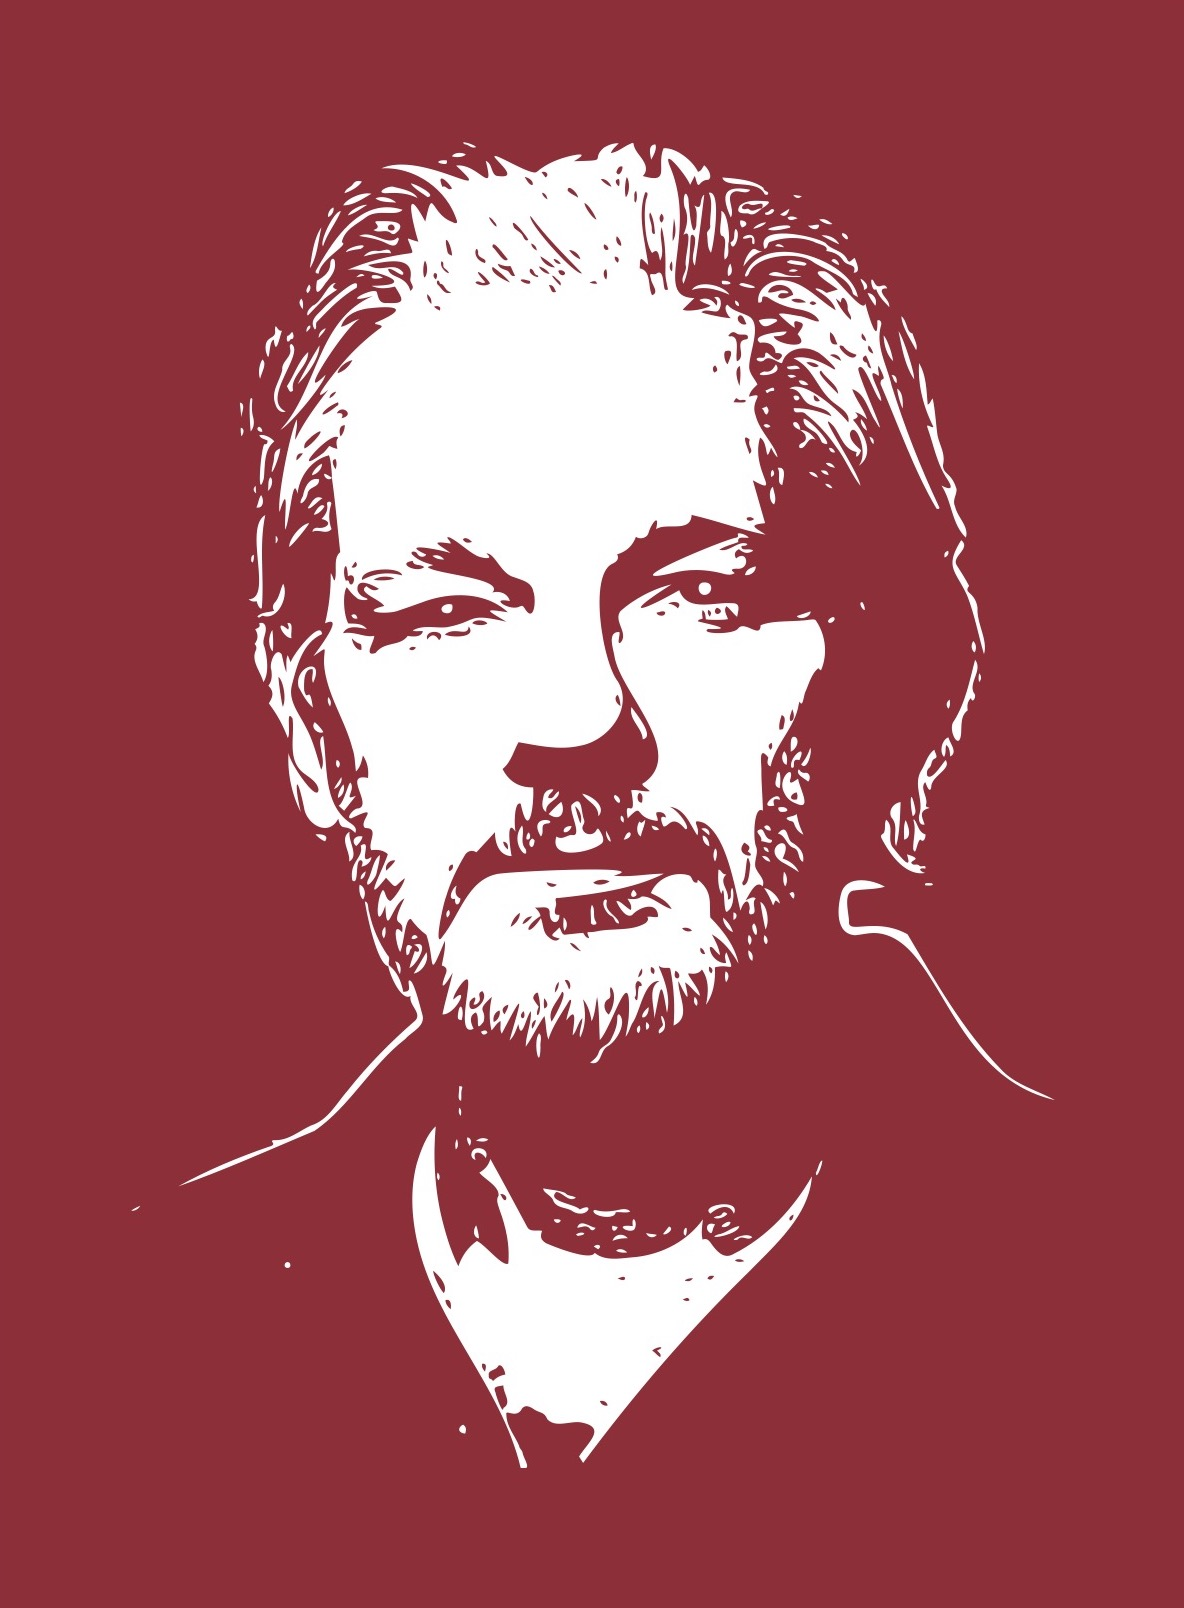
\includegraphics[width=180mm]{assange.jpg}

\newpage
\thispagestyle{empty} % No page number on this page
\vspace*{\fill}
% Herausgeber:
% Martin Sonneborn
% Fraktionsloses Mitglied des Europäischen Parlaments
% Rue Wiertz 60
% 1047 Brüssel
% Belgien
% 2. Auflage, aktualisiert. Jetzt noch deprimierender. Smiley!
% Die zum Ausdruck gebrachten Meinungen liegen in der alleinigen Verantwortung der jeweiligen Verfasser
% und geben nicht unbedingt den offiziellen Standpunkt des Europäischen Parlaments wieder.
\begin{verbatim}
Editor:
Martin Sonneborn
Non-attached Member of the European Parliament
Rue Wiertz 60
1047 Brussels
Belgium
2nd edition, updated and revised. Now even more depressing. Smiley!
The opinions expressed are the sole responsibility of the authors and do not necessarily 
reflect the official position of the European Parliament.
\end{verbatim}
\end{document}